%% SET DOCUMENT CLASS %%
% EXAM
%\documentclass[11pt,addpoints]{exam} 
%\documentclass[11pt,addpoints,answers]{exam}

% BOOK
%\documentclass[a4paper,11pt,openany,titlepage]{book}
\documentclass[a4paper,11pt,oneside]{book}

% ARTICLE
%\documentclass[11pt]{article}

% BEAMER
%\documentclass{beamer}

%% INCLUDE PREAMBLES %%
% e-TeX tools for LaTeX
\usepackage{etoolbox}

% toggle document class
\newtoggle{book}    \settoggle{book}{true}
\newtoggle{exam}    \settoggle{exam}{false}
\newtoggle{article} \settoggle{article}{false}
\newtoggle{beamer}  \settoggle{beamer}{false}

% toggle: document contains citations
\newtoggle{citations}   \settoggle{citations}{true}

% An alternative to babel for XeLaTeX and LuaLaTeX. LOAD BEFORE BIBLATEX
\usepackage{polyglossia}
\setdefaultlanguage[spelling=new, babelshorthands=true]{german}
%\setotherlanguage{latin}

% document contains citations?
%\iftoggle{citations} {
    % Sophisticated Bibliographies in LaTeX
    \usepackage[maxbibnames=99,sorting=none,style=alphabetic,backend=biber]{biblatex}

    \addbibresource{refs.bib}
%2} {}

% Run a document through LaTeX for syntax checking
%\usepackage{syntonly}

% Draw a page-layout diagram
%\usepackage{showframe}

% Advanced font selection in XeLaTeX and LuaLaTeX
\usepackage{fontspec}

% Reimplementation of and extensions to LaTeX verbatim
\usepackage{verbatim}

% is document NOT a beamer presentation?
\iftoggle{beamer} {
    %
} {
    % Flexible and complete interface to document dimensions
    \usepackage[a4paper,bindingoffset=0mm,left=30mm,right=30mm,top=25mm,bottom=25mm,footskip=15mm]{geometry}
}

% Easy access to the Lorem Ipsum dummy text
\usepackage{lipsum}

% Extensive support for hypertext in LaTeX
\usepackage{hyperref}
\hypersetup{
    colorlinks,
    linkcolor={red!40!black},
    citecolor={blue!70!black},
    urlcolor={blue!90!black}
}

\ifboolexpr{not (togl {beamer})}
{
% Control table of contents, figures, etc
\usepackage{tocloft}
}{}

\ifboolexpr{togl {exam} or togl {beamer}}
    {}
    {
        % Extensive control of page headers and footers in LaTeX2ε
        \usepackage{fancyhdr}
    }

% Completely customisable TOCs
\usepackage{etoc}

% Alternative headings for toc/lof/lot
\usepackage{titletoc}

% Conditional commands in LaTeX documents
\usepackage{ifthen}

% String manipulation for (La)TeX
\usepackage{xstring}

% Define commands that appear not to eat spaces
\usepackage{xspace}

% Context sensitive quotation facilities
\usepackage{csquotes}

% AMS mathematical facilities for LaTeX
\usepackage{amsmath}

% TeX fonts from the American Mathematical Society
\usepackage{amssymb}

% AMS-LaTeX commutative diagrams
\usepackage{amscd}

% Typesetting theorems (AMS style)
\usepackage{amsthm}

% Place lines through maths formulae
\usepackage{cancel}

% Access bold symbols in maths mode
\usepackage{bm}

% Macros for manipulating polynomials
\usepackage{polynom}

% Mathematical tools to use with amsmath
\usepackage{mathtools}

\ifboolexpr{not (togl {beamer})}
{
    % Control table of contents, figures, etc
    % Driver-independent color extensions for LaTeX and pdfLaTeX
    \usepackage[svgnames]{xcolor}
    % see 'svgnames' in:
    % https://mirror.koddos.net/CTAN/macros/latex/contrib/xcolor/xcolor.pdf
}{}

% Enhanced support for graphics
\usepackage{graphicx}

% wrapfig – Produces figures which text can flow around
\usepackage{wrapfig}

% Support for sub-captions
\usepackage{subcaption}

% Intermix single and multiple columns
\usepackage{multicol}

% Create PostScript and PDF graphics in TeX
\usepackage{tikz}
% Martin Vogel's Symbols (marvosym) font
\usepackage{marvosym}
% Some symbols created using TikZ
\usepackage[marvosym]{tikzsymbols}
\usetikzlibrary{
  3d,
  arrows,
  arrows.spaced,
  arrows.meta,
  bending,
  babel,
  calc,
  fit,
  patterns,
  patterns.meta,
  plotmarks,
  shapes.geometric,
  shapes.misc,
  shapes.symbols,
  shapes.arrows,
  shapes.callouts,
  shapes.multipart,
  shapes.gates.logic.US,
  shapes.gates.logic.IEC,
  circuits.logic.US,
  circuits.logic.IEC,
  circuits.logic.CDH,
  circuits.ee.IEC,
  datavisualization,
  datavisualization.polar,
  datavisualization.formats.functions,
  er,
  automata,
  backgrounds,
  chains,
  topaths,
  trees,
  petri,
  mindmap,
  matrix,
  calendar,
  folding,
  fadings,
  shadings,
  spy,
  through,
  turtle,
  positioning,
  scopes,
  decorations.fractals,
  decorations.shapes,
  decorations.text,
  decorations.pathmorphing,
  decorations.pathreplacing,
  decorations.footprints,
  decorations.markings,
  shadows,
  lindenmayersystems,
  intersections,
  fixedpointarithmetic,
  fpu,
  svg.path,
  external,
  graphs,
  graphs.standard,
  quotes,
  math,
  angles,
  views,
  animations,
  rdf,
  perspective,
}

% The package provides a PGF/TikZ-based mechanism for drawing linguistic (and other kinds of) trees.
\usepackage{forest}

% Create normal/logarithmic plots in two and three dimensions
\usepackage{pgfplots}
\pgfplotsset{compat=newest}

% Framed environments that can split at page boundaries
\usepackage[framemethod=TikZ]{mdframed}

% Customising captions in floating environments
\usepackage{caption}

% Improved interface for floating objects
\usepackage{float}

% A range of footnote options
\usepackage[hang, flushmargin]{footmisc}

% This package provides user control over the layout of the three basic list environments: enumerate, itemize and description.
\usepackage[shortlabels]{enumitem}
\setlist{nolistsep} % smaller spacing in lists

% A package for producing multiple indexes
\usepackage{imakeidx}

% A generic document command parser
\usepackage{xparse}

% Create PostScript and PDF graphics in TeX
\usepackage{pgf}

% defines \foreach
\usepackage{pgffor}

% This package introduces aliases for counters, that share the same counter register and ‘clear’ list. 
\usepackage{aliascnt}

% Verbatim with URL-sensitive line breaks
\usepackage{url}

% Typeset source code listings using LaTeX
\usepackage{listings}

% float wrapper for algorithms
\usepackage{algorithm}

% layout for algorithmicx
\usepackage[noend]{algpseudocode}

% Extra control of appendices
\usepackage[toc,page]{appendix}

% Change the resetting of counters
\usepackage{chngcntr}

% Highly customised stacking of objects, insets, baseline changes, etc
\usepackage{stackengine}

% Horizontally columned lists
\usepackage{tasks}

% Typeset exercises, problems, etc. and their answers
\usepackage[lastexercise,answerdelayed]{exercise}

% Intelligent cross-referencing. LOAD AFTER \hypersetup
\usepackage[nameinlink,noabbrev]{cleveref}

% left ( and right ) round brackets
\newcommand{\lr}[1]{\left(#1\right)}
% left { and right } curly brackets
\newcommand{\lrc}[1]{\left\{#1\right\}}
% left [ and right ] square brackets
\newcommand{\lrs}[1]{\left[#1\right]}
% set (condition is in math mode): {n\in\N ; n < 10}
\newcommand{\setcm}[2]{\lrc{\;#1 \; ; \; #2 \;}}
% set (condition is in text mode): {n\in\N ; $n$ is even}
\newcommand{\setct}[2]{\lrc{\;#1 \; ; \; \text{#2} \;}}
% set (all in text mode): {$w$ ist binärer String ; $n$ is even}
\newcommand{\settt}[2]{\lrc{\; \text{#1} \; ; \; \text{#2} \;}}
% N (set of natural numbers)
\newcommand{\N}{\mathbb{N}}
% set of units in N = N\{0}
\newcommand{\Nunit}{\N^{\times}}
% Z (set of integers)
\newcommand{\Z}{\mathbb{Z}}
% set of units in Z = Z\{0}
\newcommand{\Zunit}{\Z^{\times}}
% Q
\newcommand{\Q}{\mathbb{Q}}
% set of units in Q = Q\{0}
\newcommand{\Qunit}{\Q^{\times}}
% R
\newcommand{\R}{\mathbb{R}}
% set of units in R = R\{0}
\newcommand{\Runit}{\R^{\times}}
% R >= 0 (non negative real numbers)
\newcommand{\Rnn}{\R_{\geq 0}}
% R > 0 (positive real numbers)
\newcommand{\Rp}{\R_{>0}}
% C
\newcommand{\C}{\mathbb{C}}
% set of units in C = C\{0}
\newcommand{\Cunit}{\C^{\times}}
% K
\newcommand{\K}{\mathbb{K}}
% set of units in K = K\{0}
\newcommand{\Kunit}{\K^{\times}}
% real part of a complex number Re(...)
\newcommand{\real}[1]{\text{Re}\lr{#1}}
% imaginary part of a complex number Im(...)
\newcommand{\imag}[1]{\text{Im}\lr{#1}}
% absolute value
\newcommand{\abs}[1]{\left\lvert#1\right\rvert}
% norm
\newcommand{\norm}[1]{\left\lVert#1\right\rVert}
% closed interval [a,b]
\newcommand{\ic}[2]{\lrs{#1, #2}}
% closed / open interval [a,b)
\newcommand{\ico}[2]{\left[#1, #2\right)}
% open / closed interval (a,b]
\newcommand{\ioc}[2]{\left(#1, #2\right]}
% open interval (a,b)
\newcommand{\io}[2]{\lr{#1, #2}}
% double fraction
\newcommand{\doublefraction}[4]{\cfrac{\frac{#1}{#2}}{\frac{#3}{#4}}}
% degree (of a polynomial)
\newcommand{\degree}[1]{\text{Grad}\lr{#1}}
% defining symbols :=, =:  
\newcommand{\defeql}{\mathrel{\mathop:}=} % defines Symbol :=
\newcommand{\defeqr}{=\mathrel{\mathop:}} % defines Symbol =:
% ceiling operator
\newcommand{\ceil}[1]{\left \lceil #1 \right \rceil}
% floor operator
\newcommand{\floor}[1]{\left \lfloor #1 \right \rfloor}
% quotation marks
\newcommand{\quotes}[1]{``#1''}
% text italics and bold font
\newcommand{\tib}[1]{\textbf{\textit{#1}}}
% implication
\newcommand{\imp}{\Rightarrow}
% cardinality
\newcommand{\anz}[1]{\text{Anz}\lr{#1}}
% arg
\newcommand{\Carg}[1]{\text{arg}\lr{#1}}
% cis
\newcommand{\cis}[1]{\text{cis}\lr{#1}}

% Typeset source code listings using LaTeX
\lstdefinestyle{mystyle}{
    backgroundcolor=\color{BlanchedAlmond!10},   
    commentstyle=\color{Blue},
    keywordstyle=\color{Green},
    numberstyle=\tiny\color{Gray},
    stringstyle=\color{Fuchsia},
    basicstyle=\ttfamily\small,
    breakatwhitespace=false,         
    breaklines=true,                 
    captionpos=b,                    
    keepspaces=true,                 
    numbers=left,                    
    numbersep=5pt,                  
    showspaces=false,                
    showstringspaces=false,
    showtabs=false,                  
    tabsize=4
}
\lstset{style=mystyle}

% Typeset source code listings using LaTeX
\lstdefinestyle{mystyleFootnotesize}{
    backgroundcolor=\color{BlanchedAlmond!10},   
    commentstyle=\color{Blue},
    keywordstyle=\color{Green},
    numberstyle=\tiny\color{Gray},
    stringstyle=\color{Fuchsia},
    basicstyle=\ttfamily\footnotesize,
    breakatwhitespace=false,         
    breaklines=true,                 
    captionpos=b,                    
    keepspaces=true,                 
    numbers=left,                    
    numbersep=5pt,                  
    showspaces=false,                
    showstringspaces=false,
    showtabs=false,                  
    tabsize=4
}

% Typeset source code listings using LaTeX
\lstdefinestyle{mystyleTiny}{
    backgroundcolor=\color{BlanchedAlmond!10},   
    commentstyle=\color{Blue},
    keywordstyle=\color{Green},
    numberstyle=\tiny\color{Gray},
    stringstyle=\color{Fuchsia},
    basicstyle=\ttfamily\tiny,
    breakatwhitespace=false,         
    breaklines=true,                 
    captionpos=b,                    
    keepspaces=true,                 
    numbers=left,                    
    numbersep=5pt,                  
    showspaces=false,                
    showstringspaces=false,
    showtabs=false,                  
    tabsize=4
}

\crefname{lstlisting}{Programm}{Programme}
\Crefname{lstlisting}{Programm}{Programme}
\renewcommand{\lstlistingname}{Listing}

% Python for inline
\newcommand{\pythoninline}[1]{{\lstinline[language=Python]!#1!}}

% C++ for inline
\newcommand{\cppinline}[1]{{\lstinline[language=C++]!#1!}}

\floatname{algorithm}{Algorithmus}

\renewcommand{\algorithmicrequire}{\textbf{Eingabe:}}
\renewcommand{\algorithmicensure}{\textbf{Resultat:}}

% enumerate with roman numbers
\newlist{renum}{enumerate}{1}
\setlist[renum,1]{label=(\roman*)}

% enumerate alphabetically
\newlist{aenum}{enumerate}{1}
\setlist[aenum,1]{label=(\alph*)}

% custom environments
\newcounter{dc} \setcounter{dc}{99999}
\newcommand{\mylabel}{foo} % will get overwritten
\iftoggle{book} {
	\newcounter{cc}[chapter] % cc is reset at start of new chapter
} {
	\newcounter{cc}[section] % cc is reset at start of new section
}
\setcounter{cc}{0}
\iftoggle{book} {
	\renewcommand{\thecc}{\arabic{chapter}.\arabic{cc}}
} {
	\renewcommand{\thecc}{\arabic{section}.\arabic{cc}}
}

% theorem environment
\newaliascnt{ccsatz}{cc}
\aliascntresetthe{ccsatz}
\crefname{ccsatz}{Satz}{Sätze}
\Crefname{ccsatz}{Satz}{Sätze}

\newenvironment{satz}[2][]
    {
        \refstepcounter{ccsatz}
        \ifblank{#1} {
            % if no title is given (#1 blank)
        	\mdfsetup{
        	frametitle={
        	\tikz[baseline=(current bounding box.east),outer sep=0pt]
        	\node[anchor=east,rectangle,fill=Gold!60]
        	{\strut Satz~\thecc};}
        	}
        } {	
            % if a title is given (#1 not blank)
        	\mdfsetup{
        	frametitle={
        	\tikz[baseline=(current bounding box.east),outer sep=0pt]
        	\node[anchor=east,rectangle,fill=Gold!60]
        	{\strut Satz~\thecc~#1};}
        	}
        }
        \mdfsetup{
        	innertopmargin=0pt, linecolor=Gold,
        	linewidth=1pt, topline=true, frametitleaboveskip=\dimexpr-\ht\strutbox\relax
        }
        \ifstrequal{#2}{-} {
        	% #2 is the dummy label "-"
        	\renewcommand{\mylabel}{\arabic{dc}}
        	\refstepcounter{dc}
        } {
        	% #2 is an actual user-defined label
        	\renewcommand{\mylabel}{#2}
        }
        \begin{mdframed}[backgroundcolor=Gold!15]\relax%
        \label{\mylabel}
    } %%
    {
        \end{mdframed}
    }

% definition environment
\newaliascnt{ccdefinition}{cc}
\aliascntresetthe{ccdefinition}
\crefname{ccdefinition}{Definition}{Definitionen}
\Crefname{ccdefinition}{Definition}{Definitionen}

\newenvironment{definition}[2][]
    {
        \refstepcounter{ccdefinition}
        \ifblank{#1} {
            % if no title is given (#1 blank)
        	\mdfsetup{
        	frametitle={
        	\tikz[baseline=(current bounding box.east),outer sep=0pt]
        	\node[anchor=east,rectangle,fill=DarkCyan!40]
        	{\strut Definition~\thecc};}
        	}
        } {	
            % if a title is given (#1 not blank)
        	\mdfsetup{
        	frametitle={
        	\tikz[baseline=(current bounding box.east),outer sep=0pt]
        	\node[anchor=east,rectangle,fill=DarkCyan!40]
        	{\strut Definition~\thecc~#1};}
        	}
        }
        \mdfsetup{
        	innertopmargin=0pt, linecolor=DarkCyan!80,
        	linewidth=1pt, topline=true, frametitleaboveskip=\dimexpr-\ht\strutbox\relax
        }
        \ifstrequal{#2}{-} {
        	% #2 is the dummy label "-"
        	\renewcommand{\mylabel}{\arabic{dc}}
        	\refstepcounter{dc}
        } {
        	% #2 is an actual user-defined label
        	\renewcommand{\mylabel}{#2}
        }
        \begin{mdframed}[backgroundcolor=DarkCyan!8]\relax%
        \label{\mylabel}
    } %%
    {
        \end{mdframed}
    }
    
% vereinbarung environment
\newaliascnt{ccvereinbarung}{cc}
\aliascntresetthe{ccvereinbarung}
\crefname{ccvereinbarung}{Vereinbarung}{Vereinbarungen}
\Crefname{ccvereinbarung}{Vereinbarung}{Vereinbarungen}

\newenvironment{vereinbarung}[2][]
    {
        \refstepcounter{ccvereinbarung}
        \ifblank{#1} {
            % if no title is given (#1 blank)
        	\mdfsetup{
        	frametitle={
        	\tikz[baseline=(current bounding box.east),outer sep=0pt]
        	\node[anchor=east,rectangle,fill=Coral!40]
        	{\strut Vereinbarung~\thecc};}
        	}
        } {	
            % if a title is given (#1 not blank)
        	\mdfsetup{
        	frametitle={
        	\tikz[baseline=(current bounding box.east),outer sep=0pt]
        	\node[anchor=east,rectangle,fill=Coral!40]
        	{\strut Vereinbarung~\thecc~#1};}
        	}
        }
        \mdfsetup{
        	innertopmargin=0pt, linecolor=Coral!80,
        	linewidth=1pt, topline=true, frametitleaboveskip=\dimexpr-\ht\strutbox\relax
        }
        \ifstrequal{#2}{-} {
        	% #2 is the dummy label "-"
        	\renewcommand{\mylabel}{\arabic{dc}}
        	\refstepcounter{dc}
        } {
        	% #2 is an actual user-defined label
        	\renewcommand{\mylabel}{#2}
        }
        \begin{mdframed}[backgroundcolor=Coral!15]\relax%
        \label{\mylabel}
    } %%
    {
        \end{mdframed}
    }

% box environment
\newaliascnt{ccbox}{cc}
\aliascntresetthe{ccbox}
\crefname{ccbox}{Box}{Boxen}
\Crefname{ccbox}{Box}{Boxen}

\newenvironment{myBox}[2][]
    {
        \refstepcounter{ccbox}
        \ifblank{#1} {
            % if no title is given (#1 blank)
        	\mdfsetup{
        	frametitle={
        	\tikz[baseline=(current bounding box.east),outer sep=0pt]
        	\node[anchor=east,rectangle,fill=Indigo!40]
        	{\strut Box~\thecc};}
        	}
        } {	
            % if a title is given (#1 not blank)
        	\mdfsetup{
        	frametitle={
        	\tikz[baseline=(current bounding box.east),outer sep=0pt]
        	\node[anchor=east,rectangle,fill=Indigo!40]
        	{\strut Box~\thecc~#1};}
        	}
        }
        \mdfsetup{
        	innertopmargin=0pt, linecolor=Indigo!40,
        	linewidth=1pt, topline=true, frametitleaboveskip=\dimexpr-\ht\strutbox\relax
        }
        \ifstrequal{#2}{-} {
        	% #2 is the dummy label "-"
        	\renewcommand{\mylabel}{\arabic{dc}}
        	\refstepcounter{dc}
        } {
        	% #2 is an actual user-defined label
        	\renewcommand{\mylabel}{#2}
        }
        \begin{mdframed}[backgroundcolor=Indigo!8]\relax%
        \label{\mylabel}
    } %%
    {
        \end{mdframed}
    }

% exercises and answers
\newaliascnt{ccA}{cc}
\aliascntresetthe{ccA}
\iftoggle{book} {
	\newcounter{ccaufgabe}[chapter]
} {
	\newcounter{ccaufgabe}[section]
}
\setcounter{ccaufgabe}{0}
\iftoggle{book} {
	\renewcommand{\theccaufgabe}{\arabic{chapter}.\arabic{ccaufgabe}}
} {
	\renewcommand{\theccaufgabe}{\arabic{section}.\arabic{ccaufgabe}}
}

\crefname{ccaufgabe}{Aufgabe}{Aufgaben}
\Crefname{ccaufgabe}{Aufgabe}{Aufgaben}

\newenvironment{aufgabe}[2][]
    {
        \refstepcounter{ccA}
        \refstepcounter{ccaufgabe}
        \ifblank{#1} {
            % if no title is given (#1 blank)
        	\mdfsetup{
            	frametitle={
            	\tikz[baseline=(current bounding box.east),outer sep=0pt]
            	\node[anchor=east,rectangle,fill=DarkSeaGreen]{\strut Aufgabe~\theccA~(A\theccaufgabe)};},
            	innertopmargin=0pt, linecolor=DarkSeaGreen,
            	linewidth=1pt, topline=true, frametitleaboveskip=\dimexpr-\ht\strutbox\relax
            }
        } {	
            % if a title is given (#1 not blank)
        	\mdfsetup{
            	frametitle={
            	\tikz[baseline=(current bounding box.east),outer sep=0pt]
            	\node[anchor=east,rectangle,fill=DarkSeaGreen]{\strut Aufgabe~\theccA~#1~(A\theccaufgabe)};},
            	innertopmargin=0pt, linecolor=DarkSeaGreen,
            	linewidth=1pt, topline=true, frametitleaboveskip=\dimexpr-\ht\strutbox\relax
            }
        }
        \mdfsetup{
        	innertopmargin=0pt, linecolor=DarkSeaGreen,
        	linewidth=1pt, topline=true, frametitleaboveskip=\dimexpr-\ht\strutbox\relax
        }
        \ifstrequal{#2}{-} {
        	% #2 is the dummy label "-"
        	\renewcommand{\mylabel}{\arabic{dc}}
        	\refstepcounter{dc}
        } {
        	% #2 is an actual user-defined label
        	\renewcommand{\mylabel}{#2}
        }
        \begin{mdframed}[backgroundcolor=DarkSeaGreen!15]\relax%
        \label{\mylabel}
    } %%
    {
        \end{mdframed}
    }

\newenvironment{antwort}[1]
    {
        \renewcommand{\AnswerHeader}
        {
            \noindent
            \textcolor{DarkSeaGreen!65!black}{\textbf{Lösungsvorschlag}} zu \cref{#1} auf (ab) \cpageref{#1}:\\
            \noindent
        }
        \begin{Answer}
    } %%
    {
        \end{Answer}
    }

% examples
\newaliascnt{ccbeispiele}{cc}
\aliascntresetthe{ccbeispiele}
\crefname{ccbeispiele}{Beispiel}{Beispiele}
\Crefname{ccbeispiele}{Beispiel}{Beispiele}

\makeatletter
\newcommand{\beispiele}[3] {
	\refstepcounter{ccbeispiele}
	\IfEq{#1}{-}
	{
		% no user-defined label given (only "-")
		\renewcommand{\mylabel}{\arabic{dc}}
		\refstepcounter{dc}
	} {
		% actual user-defined label given
		\renewcommand{\mylabel}{#1}
	}
	% do not reference to this if label "-" is given
	\label{\mylabel}\par\smallskip\noindent\textbf{Beispiele~\thecc}\par\noindent #2 \begin{aenum}\item #3\checkNextArgOne}
	\newcommand{\checkNextArgOne}{\@ifnextchar\bgroup{\getNextArgOne}{\end{aenum}}}
	\newcommand{\getNextArgOne}[1]{\item #1\@ifnextchar\bgroup{\getNextArgOne}{~$_\blacktriangle$\smallskip\end{aenum}}
}
\makeatother

% example
\newaliascnt{ccbeispiel}{cc}
\aliascntresetthe{ccbeispiel}
\crefname{ccbeispiel}{Beispiel}{Beispiele}
\Crefname{ccbeispiel}{Beispiel}{Beispiele}

\newcommand{\beispiel}[2] {
	\refstepcounter{ccbeispiel}
	\IfEq{#1}{-}
	{
		% no user-defined label given (only "-")
		\renewcommand{\mylabel}{\arabic{dc}}
		\refstepcounter{dc}
	} {
		% actual user-defined label given
		\renewcommand{\mylabel}{#1}
	}
	% do not reference to this if label "-" is given
	\label{\mylabel}\par\smallskip\noindent\textbf{Beispiel~\thecc}\quad #2 ~$_\blacktriangle$\smallskip
}

% proof
\newcommand{\beweis}[1]{\smallskip\noindent\textbf{Beweis:}\quad #1 ~$_\blacksquare$\smallskip}

% multiple clever-refs
\makeatletter
\newcommand{\getNextArgTwoComma}[1]{,~\hyperref[#1]{\ref*{#1}}\@ifnextchar\bgroup{\getNextArgTwoComma}{\nolinebreak\xspace}}
\newcommand{\cleverPart}[1]{\hyperref[#1]{\namecref{#1}~\labelcref*{#1}}\getNextArgTwoComma}
\newcommand{\cleverParts}[1]{\hyperref[#1]{\namecrefs{#1}~\labelcref*{#1}}\getNextArgTwoComma}
\makeatother

% remarks
\newaliascnt{ccbemerkungen}{cc}
\aliascntresetthe{ccbemerkungen}
\crefname{ccbemerkungen}{Bemerkung}{Bemerkungen}
\Crefname{ccbemerkungen}{Bemerkung}{Bemerkungen}

\makeatletter
\newcommand{\bemerkungen}[3] {
	\refstepcounter{ccbemerkungen}
	\IfEq{#1}{-}
	{
		% no user-defined label given (only "-")
		\renewcommand{\mylabel}{\arabic{dc}}
		\refstepcounter{dc}
	} {
		% actual user-defined label given
		\renewcommand{\mylabel}{#1}
	}
	% do not reference to this if label "-" is given
	\label{\mylabel}\par\smallskip\noindent\textbf{Bemerkungen~\thecc}\par\noindent #2 \begin{aenum}\item #3\checkNextArgOne
}
\makeatother

% remark
\newaliascnt{ccbemerkung}{cc}
\aliascntresetthe{ccbemerkung}
\crefname{ccbemerkung}{Bemerkung}{Bemerkungen}
\Crefname{ccbemerkung}{Bemerkung}{Bemerkungen}

\newcommand{\bemerkung}[2] {
	\refstepcounter{ccbemerkung}
	\IfEq{#1}{-}
	{
		% no user-defined label given (only "-")
		\renewcommand{\mylabel}{\arabic{dc}}
		\refstepcounter{dc}
	} {
		% actual user-defined label given
		\renewcommand{\mylabel}{#1}
	}
	% do not reference to this if label "-" is given
	\label{\mylabel}\par\smallskip\noindent\textbf{Bemerkung~\thecc}\quad #2 ~$_\blacktriangle$\smallskip
}

% axiome
\iftoggle{book} {
	\newcounter{caxiome}[chapter]
} {
	\newcounter{caxiome}[section]
}

\setcounter{caxiome}{0}
\iftoggle{book} {
	\renewcommand{\thecaxiome}{\arabic{chapter}.\arabic{caxiome}}
} {
	\renewcommand{\thecaxiome}{\arabic{section}.\arabic{caxiome}}
}

\crefname{caxiome}{Axiom}{Axiome}
\Crefname{caxiome}{Axiom}{Axiome}

\makeatletter
\newcommand{\axiome}[3] {
	\refstepcounter{caxiome}
	\IfEq{#1}{-}
	{
		% no user-defined label given (only "-")
		\renewcommand{\mylabel}{\arabic{caxiome}}
		\refstepcounter{caxiome}
	} {
		% actual user-defined label given
		\renewcommand{\mylabel}{#1}
	}
	% do not reference to this if label "-" is given
	\label{\mylabel}\par\smallskip\noindent\textbf{Axiome~\thecaxiom}\par\noindent #2 \begin{aenum}\item #3\checkNextArgOne
}
\makeatother

% gedankenanstoss
\newcommand{\gedankenanstoss}[1]{\bigskip\noindent\textbf{Gedankenanstoss}\quad #1 \par\noindent\hspace{0.9\linewidth}$^\blacktriangle$\bigskip}

% axiom
\newaliascnt{caxiom}{caxiome}
\aliascntresetthe{caxiom}
\crefname{caxiom}{Axiom}{Axiome}
\Crefname{caxiom}{Axiom}{Axiome}

\newcommand{\axiom}[2] {
	\refstepcounter{caxiom}
	\IfEq{#1}{-}
	{
		% no user-defined label given (only "-")
		\renewcommand{\mylabel}{\arabic{caxiom}}
		\refstepcounter{caxiom}
	} {
		% actual user-defined label given
		\renewcommand{\mylabel}{#1}
	}
	% do not reference to this if label "-" is given
	\label{\mylabel}\par\smallskip\noindent\textbf{Axiom~\thecaxiom}\quad #2 ~$_\blacktriangle$\smallskip
}

\iftoggle{book}{
    % BOOK ENVIRONMENT %
    \setcounter{secnumdepth}{5}
    \setcounter{tocdepth}{5}
    % roman chapter numbering instead of normal numbering
    %\renewcommand{\thechapter}{\Roman{chapter}}
    % start chapter numbering at 0
    \setcounter{chapter}{-1}
    % slightly changing chapter marking in header
    \renewcommand{\chaptermark}[1]{\markboth{\textnormal{\thechapter}\ \textnormal{#1}}{}}
    % slightly changing section marking in header
    \renewcommand{\sectionmark}[1]{\markright{\textnormal{\thesection}\ \textnormal{#1}}{}}
    % remove chapter counter in front of section number
    %\counterwithout{section}{chapter}
    % no page number on first page of new chapter
    %\patchcmd{\chapter}{plain}{empty}{}{}
    % resetting the section counter with the start of a new chapter
    %\counterwithin{section}{chapter}
    % do not show chapter number in section numbering
    %\renewcommand*\thesection{\arabic{section}}
    % making header of toc non italics (\upshape) and not all capitals
    \addto\captionsgerman{\renewcommand{\contentsname}{\upshape{I\MakeLowercase{nhaltsverzeichnis}}}}
    % chapter quote at beginning of chapter
    \makeatletter
    \newenvironment{chapquote}[2][2em]
      {\setlength{\@tempdima}{#1}%
       \def\chapquote@author{#2}%
       \parshape 1 \@tempdima \dimexpr\textwidth-2\@tempdima\relax%
       \itshape}
      {\par\normalfont\hfill--\ \chapquote@author\hspace*{\@tempdima}\vspace{1.0cm}\ignorespacesafterend\par\noindent\aftergroup\@doendeq}
    \makeatother
}{}

\iftoggle{exam}{
    % EXAM ENVIRONMENT %
    \pointpoints{Punkt}{Punkte}
    \bonuspointpoints{Bonuspunkt}{Bonuspunkte}
    \renewcommand{\solutiontitle}{\noindent\textbf{Lösung:}\enspace}
    \hqword{Aufgabe:}
    \hpgword{Seite:}
    \hpword{Punkte:}
    \hsword{erhalten:}
    \htword{Total} 
    \bhqword{Aufgabe:}
    \bhpgword{Seite:}
    \bhpword{Bonuspunkte:}
    \bhsword{erhalten:}
    \bhtword{Total} 
    \chqword{Aufgabe:}
    \chpgword{Seite:}
    \chpword{Punkte:}
    \chbpword{Bonuspunkte:}
    \chsword{erhalten:}
    \chtword{Total} 
    %\checkedchar{\CheckedBox}
    \totalformat{Aufgabe \thequestion\ total: \totalpoints\ Punkte}
    \runningheadrule
    %\firstpageheader{\mycourse}{\myclass}{\mydate}
    \runningheader{\mycourse}{\myclass}{\mydate}
    \firstpagefooter{}{\thepage\,/\,\numpages}{}
    \runningfooter{}{\thepage\,/\,\numpages}{}
    
    \CorrectChoiceEmphasis{\normalfont}
    
    %\renewcommand{\questionlabel}{\bfseries Aufgabe~\thequestion.}
}{}




\tikzset{block/.style={
        font=\sffamily,
        draw=black,
        thin,
        fill=pink!50,
        rectangle split,
        rectangle split horizontal,
        rectangle split parts=#1,
        outer sep=0pt},
        %
        gblock/.style={
            block,
            rectangle split parts=#1,
            fill=green!30}
        }

% to highlight matrix entries with tikz
\tikzset{%
  highlight/.style={rectangle,rounded corners,fill=cyan!15,draw=none,
    fill opacity=0.4,thick,inner sep=0pt}
}
\newcommand{\tikzmark}[2]{\tikz[overlay,remember picture,
  baseline=(#1.base)] \node (#1) {#2};}
%
\newcommand{\Highlight}[1][submatrix]{%
    \tikz[overlay,remember picture]{
    \node[highlight,fit=(left.north west) (right.south east)] (#1) {};}
}

\usepackage{drawmatrix}

%\usepackage{mathpazo}
\newcounter{row}
\newcounter{col}

\newcommand\setrow[9]{
  \setcounter{col}{1}
  \foreach \n in {#1, #2, #3, #4, #5, #6, #7, #8, #9} {
    \edef\x{\value{col} - 0.5}
    \edef\y{9.5 - \value{row}}
    \node[anchor=center] at (\x, \y) {\n};
    \stepcounter{col}
  }
  \stepcounter{row}
}

\newcommand\setminirow[4]{
  \setcounter{col}{1}
  \foreach \n in {#1, #2, #3, #4} {
    \edef\x{\value{col} - 0.5}
    \edef\y{4.5 - \value{row}}
    \node[anchor=center] at (\x, \y) {\n};
    \stepcounter{col}
  }
  \stepcounter{row}
}

\usepackage{twemojis}
\usepackage{ifsym}

\newcommand{\romanNumeral}[1]{%
  \textup{\uppercase\expandafter{\romannumeral#1}}%
}

\usepackage{physics}
\usepackage{tikz-3dplot}
\usepackage[outline]{contour} % glow around text

\iftoggle{book} {
	\makeindex[columns=1,title=Index,intoc]
	%\includeonly{kapitel06}
} {}

\begin{document}
	% BOOK
	\iftoggle{book} {
	    \frontmatter
		\begin{titlepage}
    \thispagestyle{empty}
    \begin{center}
        \vspace*{1cm}
            
        {\Huge
        \textbf{Induktion und Rekursion}
            
        \vspace{0.5cm}
        \LARGE
        Mentorierte Arbeit im Lehrdiplom Informatik
            
        \vspace{1.5cm}
            
        \textbf{Erstellt von Thomas Graf unter Betreuung von Prof. Dr. Juraj Hromkovič.}
        }
        \vfill
        \clearpage
        \thispagestyle{empty}
        \mbox{}
        \vfill
        {\Large Diese Unterlagen entstanden in den Jahren 2022 / 2023 im Rahmen einer \textit{mentorierten Arbeit} im Lehrdiplom Informatik an der ETH Zürich.}

        \noindent
        Die aktuelle Version dieser Arbeit kann unter
        \begin{center}
            {\footnotesize
                \url{https://github.com/ThomasGrafNumerics/EducationalMaterial/tree/main/Mentorierte_Arbeit_Induktion_Rekursion}
            }
        \end{center}
        gefunden werden. Über inhaltliche Verbesserungsvorschläge (mittels Pull-Requests oder per E-Mail an \href{mailto:thomas.graf.education@proton.me}{thomas.graf.education@proton.me}) freuen wir uns sehr!
        \vspace{0.8cm}
    \end{center}
\end{titlepage}

		\chapter*{Vorwort}
%\addcontentsline{toc}{chapter}{Vorwort}
 
\section*{Inhalt dieser Unterlagen}
Der Fokus dieses Textes liegt auf dem Vermitteln eines fundierten Verständnisses der Prinzipien der vollständigen Induktion und der rekursiven Definition. Wir zeigen auf, wie diese beiden Prinzipien zusammenhängen und wozu sie nützlich sind.

Die sieben Kapitel dieses Skripts sind in zwei grossen Teile \textit{Mathematische Diskussion} (\cref{ch:Kapitel00,ch:Kapitel01,ch:Kapitel02,ch:Kapitel03}) und \textit{Ausgewählte rekursive Probleme und Algorithmen} (\cref{ch:Kapitel04,ch:Kapitel05,ch:Kapitel06}) gegliedert. 

\cref{ch:Kapitel00} behandelt einiges an Vorwissen, welches im Verlauf des Skripts benötigt wird. In \cref{ch:Kapitel01} beginnen wir mit der Definition der natürlichen Zahlen durch die Peano-Axiome, von welchen eines \textit{Induktionsaxiom} genannt wird. \cref{ch:Kapitel02} befasst sich mit den weitreichenden direkten Konsequenzen dieses Induktionsaxioms. In \cref{ch:Kapitel03} tasten wir uns an rekursive Definition heran und beweisen einen mächtigen Satz zum Prinzip der rekursiven Definition. Schliesslich befassen wir uns in diesem Kapitel damit, wie rekursive Funktionen in Rechnern realisiert werden können. Die letzten drei \cref{ch:Kapitel04,ch:Kapitel05,,ch:Kapitel06} beinhalten ausgewählte Anwendungen der im ersten Teil entwickelten Theorie.

\section*{Vorwissen und Zielpublikum}
%\addcontentsline{toc}{sec}{Zielpublikum}
In vielen Unterlagen werden die Themen der Induktion und Rekursion separat und scheinbar unabhängig voneinander behandelt. Zudem wird gerade die Rekursion häufig nur anhand von Beispielen gelehrt. Für dieses Skript haben wir uns zum Ziel genommen, die beiden Prinzipien auf mathematisch solide Fundamente zu stellen und ihren Zusammenhang zu verdeutlichen. Um dieses ambitionierte Ziel zu erreichen, waren wir von Anfang an bereit, einen (für das Gymnasiums) hohen Grad an Schwierigkeit und abstrakten Formalismus in Kauf zu nehmen.

Diese Unterlagen richten sich an Lernende des letzten Jahres des Gymnasiums. Besonders geeignet sind die Unterlagen für den Unterricht mit besonders leistungsfähigen Lernenden (zum Beispiel in einem Ergänzungsfach der Informatik).

Einige besondere Vorkenntnisse werden in \cref{ch:Kapitel00} eingeführt. Insbesondere sollten die Lernenden aber sicherlich die folgenden Voraussetzungen zur erfolgreichen Bearbeitung dieses Skripts mitbringen:
\begin{itemize}
	\item Sie haben Kenntnisse einer Programmiersprache (in den Unterlagen wird Python verwendet).
	\item Sie sind vertraut mit den Grundlagen der Mathematik, welche man in den ersten drei Jahren eines Kurzzeitgymnasiums erlernt.
	\item Sie kennen den Begriff der \textit{Laufzeit} eines Algorithmus und sind vertraut mit der \textit{Landau-Notation}.
\end{itemize}

\section*{Arbeiten mit diesen Unterlagen und Abhängigkeiten der Kapitel}
%\addcontentsline{toc}{sec}{Arbeiten mit diesen Unterlagen}
Die drei \cref{ch:Kapitel01,ch:Kapitel02,ch:Kapitel03} im ersten Teil (\textit{Mathematische Diskussion}) sollten nacheinander gelesen und bearbeitet werden. \cref{ch:Kapitel02} baut auf \cref{ch:Kapitel01} auf und \cref{ch:Kapitel03} auf den vorgängigen Kapiteln. Die drei \cref{ch:Kapitel04,ch:Kapitel05,ch:Kapitel06} im zweiten Teil (\textit{Ausgewählte rekursive Probleme und Algorithmen}) bauen zwar alle auf der Theorie des ersten Teils auf, besitzen aber untereinander keine Abhängigkeit. So kann beispielsweise \cref{ch:Kapitel06} problemlos bearbeitet werden, ohne die \cref{ch:Kapitel04,ch:Kapitel05} gelesen zu haben.

Mit einem Ausrufezeichen \enquote{!} markierte Elemente (Kapitel, Abschnitte, Unterabschnitte, Aufgaben) sind besonders anspruchsvoll. Die Bearbeitung und das Lesen eines mit einem Stern \enquote{*} markierten Elements ist optional. Diese \textit{optionalen} Elemente sind nicht essenziell für das Verständnis der ihnen nachfolgenden Teile.

\section*{Zeitlicher Aufwand}
Wir geben eine Aufstellung der ungefähr zu erwartenden Lektionenzahl für jedes Kapitel an. In dieser Zeit wird es nicht allen Lernenden möglich sein, sämtliche Aufgaben zu lösen.
\begin{description}
	\item[Kapitel 0 (Vorwissen):] 2 Lektionen
	\item[Kapitel 1 (Die natürlichen Zahlen):] 5 Lektionen
	\item[Kapitel 2 (Das Induktionsprinzip):] 12 Lektionen
	\item[Kapitel 3 (Rekursion):] 12 Lektionen
	\item[Kapitel 4 (Binäre Strings ohne aufeinanderfolgende Einsen):] 3 Lektionen
	\item[Kapitel 5 (Sortieren):] 5 Lektionen
	\item[Kapitel 6 (Sudoku und Backtracking):] 5 Lektionen
	\item[Appendix (Prinzip der rekursiven Definition):] 5 Lektionen
\end{description}
		\tableofcontents
        \markright{}
        \cleardoublepage
		\mainmatter
		
		\part{Mathematische Diskussion}
		\chapter{Vorwissen}\label{ch:Kapitel00}
Diese Unterlagen behandeln anspruchsvolle Inhalte der Informatik und Mathematik. Um ihnen gerecht zu werden, bedarf es einer mathematisch präzisen Ausdrucksweise. Den überwiegenden Teil der benötigten mathematischen Werkzeuge werden die Lesenden typischerweise in den ersten Jahren des Gymnasiums kennengelernt haben. Einige der von uns benötigten Konzepte werden den meisten Lesenden jedoch vermutlich noch nicht bekannt sein. Diese Konzepte wollen wir in diesem Kapitel einführen. Wir werden dies in kompakter Form tun und an verschiedenen Stellen auf artifiziell wirkende (forcierte) Beispiele bewusst verzichten.

\section{Mathematik}
\subsection{Direkter und indirekter Beweis}
Seien $A$ und $C$ mathematische Aussagen. Wir möchten beweisen, dass die Aussage
\begin{align*}
    A\Rightarrow C
\end{align*}
($A$ impliziert $C$) gilt. Solch ein Beweis kann im Wesentlichen auf zwei Arten erbracht werden: entweder durch einen \tib{direkten Beweis}\index{Beweis!direkter} oder einen \tib{indirekten Beweis}\index{Beweis!indirekter}.

\subsubsection{Direkter Beweis}
Der direkte Beweis macht von folgender logischen Tatsache Gebrauch: Impliziert $A$ eine weitere Aussage $B$
\begin{align*}
    A \Rightarrow B
\end{align*}
und $B$ impliziert wiederum $C$:
\begin{align*}
    B \Rightarrow C,
\end{align*}
dann impliziert $A$ auch $C$. Zusammengefasst gilt also:
\begin{align}\label{eq:direkterBeweis}
     \lr{\textcolor{Blue}{(A\Rightarrow B) \text{ und } (B\Rightarrow C)}} \Rightarrow \lr{\textcolor{Green}{A\Rightarrow C}}.
\end{align}
Um die Richtigkeit der Implikation $A\Rightarrow C$ zu beweisen, zerlegt man die Implikation in bereits als für richtig befundene \enquote{Teilaussagen} $A\Rightarrow B$ und $B\Rightarrow C$, also
\begin{align*}
    \textcolor{Blue}{(A\Rightarrow B) \text{ und } (B\Rightarrow C)}.
\end{align*}
Danach folgt die Implikation $\textcolor{Green}{A\Rightarrow C}$ aus Ausdruck \ref{eq:direkterBeweis}. Diese Strategie kann wiederholt angewendet werden und man erhält eine \enquote{Kette} logischer Implikationen (Schlüsse):
\begin{align*}
    \lr{ \textcolor{Blue}{(A\Rightarrow B_1) \text{ und } (B_1\Rightarrow B_2) \text{ und } (B_2\Rightarrow B_3) \text{ und } \ldots \text{ und } (B_n\Rightarrow C)} } \Rightarrow (\textcolor{Green}{A\Rightarrow C}).
\end{align*}
Dabei können die Begründungen der Implikationen $A\Rightarrow B_1$, $B_n\Rightarrow C$ sowie $B_k\Rightarrow B_{k+1}$ für jedes $k\in\lrc{1,2,\ldots, n-1}$ als logische \enquote{Zwischenschritte} verstanden werden.

\subsubsection{Indirekter Beweis}
Ein indirekter Beweis (Beweis durch Widerspruch) beginnt mit der Annahme, dass die Aussage $C$ falsch sei, dass also $\neg{C}$ (nicht $C$) richtig ist. Nun wird einzig, unter Verwendung der Richtigkeit von $A$ und $\neg{C}$ sowie bereits als wahr erkannter mathematischer Aussagen, die Richtigkeit einer Aussage $B$ abgeleitet, von der bereits bekannt ist, dass sie falsch ist. Dadurch haben wir einen \enquote{Widerspruch} erhalten und können folgern, dass $\neg{C}$ nicht richtig sein kann und somit $C$ wahr sein muss. Damit ist, wie gewünscht, die Implikation $A\Rightarrow C$ nachgewiesen.

\subsection{Kontraposition}
Seien $A$ und $B$ mathematische Aussagen. Logisch äquivalent zur Behauptung $A\Rightarrow B$ ist die Aussage $\neg{B}\Rightarrow \neg{A}$, welche \tib{Kontraposition}\index{Kontraposition} der Implikation $A\Rightarrow B$ genannt wird. Der Beweis für $A\Rightarrow B$ ist demnach auch erbracht, falls man zeigen kann, dass aus der Annahme, die Folgerungen seien nicht erfüllt, folgt, dass auch die Voraussetzungen nicht erfüllt sein können. Gelegentlich fällt es einem leichter, die Kontraposition $\neg{B}\Rightarrow \neg{A}$ einer Implikation $A\Rightarrow B$ zu zeigen.

\beispiel{-}
{Sei $A$ die Aussage \enquote{Es hat geregnet.} und $B$ die Aussage \enquote{Die Strasse ist nass.}. Die Implikation $A\Rightarrow B$ bedeutet: \enquote{Falls es geregnet hat, ist die Strasse nass.}

\noindent
Falls die Strasse nass ist, muss das umgekehrt nicht bedeuten, dass es geregnet hat. Beispielsweise könnte die Strasse auch von der Strassenreinigung nass gemacht worden sein. Was wir aber sicherlich sagen können, ist, dass falls die Strasse \textit{nicht} nass ist, es auch \textit{nicht} geregnet haben kann, was genau 
$\neg{B}\Rightarrow \neg{A}$ bedeutet.
}

\subsection{Funktionen}
\subsubsection{Definition einer Funktion (*)}
\begin{definition}[Funktion als Vorschrift]{definition:funktion}
Seien $X$ und $Y$ Mengen. Wir sagen, dass eine \tib{Funktion}\index{Funktion} auf $X$ mit Werten in $Y$ definiert ist, wenn aufgrund einer \textit{Vorschrift} (\textit{Regel}) $f$ jedem Element $x\in X$ genau ein Element $y\in Y$ zugehörig ist.
\end{definition}
Wir sagen dann, dass die Menge $X$ die \tib{Definitionsmenge}\index{Funktion!Defintionsmenge einer} der Funktion ist.

Das Symbol $x$, das benutzt wird, um ein allgemeines Element dieser Menge zu beschreiben, wird \tib{Argument}\index{Funktion!Argument einer} oder \textit{unabhängige Variable} der Funktion genannt.

Das Element $y_0\in Y$, das einem Argument $x_0\in X$ zugeordnet wird, wird \tib{Wert}\index{Funktion!Wert einer} der Funktion in $x_0$ genannt oder auch Wert der Funktion an der Stelle $x = x_0$ und $f(x_0)$ geschrieben. Die Menge $Y$ wird \tib{Zielmenge}\index{Funktion!Zielmenge einer} der Funktion genannt.

Bei Änderung der Argumente $x\in X$ verändern sich im Allgemeinen die Resultate $y = f(x)\in Y$ in Abhängigkeit von den Werten $x$. Aus diesem Grund wird die Grösse $y=f(x)$ oft auch \textit{abhängige Variable} genannt.
\begin{definition}[Bild einer Funktion]{definition:bild}
Die Menge
\begin{align*}
    \text{im}\lr{f} := \setct{y\in Y}{es existiert ein $x\in X$ mit $y=f(x)$}
\end{align*}
von Werten, die von einer Funktion $f$ für alle Elemente in der Menge $X$ angenommen werden, wird \tib{Bild} (englisch: \textit{image}) oder \textit{Wertemenge} der Funktion $f:X\to Y$ genannt. Häufig wird $\text{im}\lr{f}$ alternativ als $f(X)$ geschrieben, wobei $X$ die Definitionsmenge von $f$ ist.
\end{definition}

\subsubsection{Surjektion, Injektion, Bijektion}
In diesen Unterlagen werden wir häufig über Funktionen sprechen. Insbesondere werden wir die folgenden drei Eigenschaften von Funktionen mehrmals verwenden.
\begin{definition}[surjektiv, injektiv, bijektiv]{definition:eigenschaftenFunktionen}
Seien $X$ und $Y$ Mengen und $f: X\to Y$ eine Funktion.
\begin{itemize}
    \item $f$ heisst \tib{surjektiv}\index{Funktion!surjektive} (eine \textit{Surjektion}), falls $\text{im}\lr{f} = Y$.
    
    \textcolor{Gray}{Intuitiv gesprochen, nimmt eine surjektive Funktion jeden Wert in der Zielmenge an. Zu beliebigem $y\in Y$ existiert (mindestens) ein $x\in X$, sodass $y=f(x)$.}
    \item $f$ heisst \tib{injektiv}\index{Funktion!injektive} (eine \textit{Injektion}), falls für $x_1,x_2\in X$ aus $x_1\neq x_2$ stets $f(x_1)\neq f(x_2)$ folgt.
    
    \textcolor{Gray}{Zwei verschiedene Eingaben erzeugen stets verschiedene Ausgaben.}
    \item $f$ heisst \tib{bijektiv}\index{Funktion!bijektive} (eine \textit{Bijektion}), falls $f$ sowohl surjektiv als auch injektiv ist.
    
    \textcolor{Gray}{Da $f$ surjektiv ist, existiert zu jedem $y\in Y$ ein $x\in X$ mit $f(x)=y$. Da $f$ injektiv ist, kann es kein anderes $\tilde{x}\in X$ mit $\tilde{x}\neq x$ geben, sodass $f(\tilde{x})=y$. Dadurch stellt eine Bijektion eine \enquote{Eins-zu-eins-Zuweisung} zwischen den Elementen aus $X$ und $Y$ dar.}
\end{itemize}
\end{definition}

\begin{figure}[H]
    \centering
    \begin{subfigure}[b]{0.30\textwidth}
        \begin{tikzpicture}[scale=0.8]
            \draw (0,0) -- node[below] {$X$} (5,0) -- (5,3) -- (0,3) -- node[left] {$Y$} (0,0);
            \draw (0,1.2) to [out=60,in=190] (1,3) to [out=360,in=110] (3,1) to [out=290,in=170] (5,0);
        \end{tikzpicture}
        \caption{surjektiv, nicht injektiv}
        \label{subfig:surjektiv}
    \end{subfigure}
    \begin{subfigure}[b]{0.30\textwidth}
        \begin{tikzpicture}[scale=0.8]
            \draw (0,0) -- node[below] {$X$} (5,0) -- (5,3) -- (0,3) -- node[left] {$Y$} (0,0);
            \draw (0,0.2) to [out=40,in=190] (5,2.5);
        \end{tikzpicture}
        \caption{injektiv, nicht surjektiv}
        \label{subfig:injektiv}
    \end{subfigure}
    \begin{subfigure}[b]{0.30\textwidth}
        \begin{tikzpicture}[scale=0.8]
            \draw (0,0) -- node[below] {$X$} (5,0) -- (5,3) -- (0,3) -- node[left] {$Y$} (0,0);
            \draw (0,0) to [out=15,in=250] (5,3);
        \end{tikzpicture}
        \caption{bijektiv}
        \label{subfig:bijektiv}
    \end{subfigure}%
    \caption{schematische Darstellung der Eigenschaften in \cref{definition:eigenschaftenFunktionen}}
    \label{fig:surinjbi}
\end{figure} 

\begin{figure}[H]
    \centering
    \begin{subfigure}[b]{0.30\textwidth}
        \begin{tikzpicture}[scale=0.8]
            % draw the sets
            \filldraw[fill=blue!20, draw=blue!60] (-1.5,0) circle (1.3cm);
            \filldraw[fill=red!20, draw=red!60] (1.5,0) circle (1cm);
            % the texts
            \node at (-1.5,1.7) {$X$};
            \node at (1.5,1.4) {$Y$};
            % the points in the sets (here I just create nodes to use them later on to position
            % the circles and the arrows
            \node (x1) at (-1.5,1.0) {$1$};
            \node (x2) at (-1.5,0.5) {$23$};
            \node (x3) at (-1.5,0.0) {$9$};
            \node (x4) at (-1.5,-0.5) {$7$};
            \node (x5) at (-1.5,-1.0) {$4$};
            
            \node (y1) at (1.5,0.7) {$7$};
            \node (y2) at (1.5,0.2) {$30$};
            \node (y3) at (1.5,-0.3) {$0$};
            \node (y4) at (1.5,-0.8) {$6$};
        
            % draw the arrows
            \draw[-stealth] (x1) -- (y2);
            \draw[-stealth] (x2) -- (y1);
            \draw[-stealth] (x3) -- (y2);
            \draw[-stealth] (x4) -- (y3);
            \draw[-stealth] (x5) -- (y4);
        \end{tikzpicture}
        \caption{surjektiv, nicht injektiv}
        \label{subfig:surjektivDiagramm}
    \end{subfigure}
    \begin{subfigure}[b]{0.30\textwidth}
        \begin{tikzpicture}[scale=0.8]
            \filldraw[fill=blue!20, draw=blue!60] (-1.5,0) circle (1cm);
            \filldraw[fill=red!20, draw=red!60] (1.5,0) circle (1.3cm);
        
            \node at (-1.5,1.4) {$X$};
            \node at (1.5,1.7) {$Y$};
        
            \node (x1) at (-1.5,0.7) {$1$};
            \node (x2) at (-1.5,0.2) {$4$};
            \node (x3) at (-1.5,-0.3) {$0$};
            \node (x4) at (-1.5,-0.8) {$6$};
            
            \node (y1) at (1.5,1.0) {$1$};
            \node (y2) at (1.5,0.5) {$9$};
            \node (y3) at (1.5,0.0) {$8$};
            \node (y4) at (1.5,-0.5) {$7$};
            \node (y5) at (1.5,-1.0) {$4$};
        
            \draw[-stealth] (x1) -- (y3);
            \draw[-stealth] (x2) -- (y1);
            \draw[-stealth] (x3) -- (y4);
            \draw[-stealth] (x4) -- (y5);
        \end{tikzpicture}
        \caption{injektiv, nicht surjektiv}
        \label{subfig:injektivDiagramm}
    \end{subfigure}
    \begin{subfigure}[b]{0.30\textwidth}
        \begin{tikzpicture}[scale=0.8]
            \filldraw[fill=blue!20, draw=blue!60] (-1.5,0) circle (1cm);
            \filldraw[fill=red!20, draw=red!60] (1.5,0) circle (1cm);
        
            \node at (-1.5,1.4) {$X$};
            \node at (1.5,1.4) {$Y$};
        
            \node (x1) at (-1.5,0.7) {$10$};
            \node (x2) at (-1.5,0.2) {$3$};
            \node (x3) at (-1.5,-0.3) {$15$};
            \node (x4) at (-1.5,-0.8) {$1$};
            
            \node (y1) at (1.5,0.7) {$1$};
            \node (y2) at (1.5,0.2) {$5$};
            \node (y3) at (1.5,-0.3) {$8$};
            \node (y4) at (1.5,-0.8) {$15$};
        
            \draw[-stealth] (x1) -- (y3);
            \draw[-stealth] (x2) -- (y2);
            \draw[-stealth] (x3) -- (y4);
            \draw[-stealth] (x4) -- (y1);
        \end{tikzpicture}
        \caption{bijektiv}
        \label{subfig:bijektivDiagramm}
    \end{subfigure}
    \caption{Diagramm-Darstellung der Eigenschaften in \cref{definition:eigenschaftenFunktionen}}
    \label{fig:diagsurinjbi}
\end{figure} 

\noindent
Betrachten Sie \cref{fig:surinjbi}. Diese stellt die in \cref{definition:eigenschaftenFunktionen} beschriebenen Eigenschaften für eine Funktion $f:X\to Y$ schematisch dar. \cref{subfig:surjektiv} zeigt eine Funktion, die surjektiv, aber nicht injektiv ist, \cref{subfig:injektiv} eine Funktion, die injektiv, aber nicht surjektiv ist. Schliesslich wird in \cref{subfig:bijektiv} eine bijektive Funktion dargestellt. \cref{fig:diagsurinjbi} illustriert Surjektivität, Injektivität und Bijektivität für einfache Funktionen auf konkreten endlichen Mengen. Surjektivität, Injektivität und Bijektivität sind Eigenschaften, welche eine gegebene Funktion entweder haben kann oder nicht.

\subsubsection{Folgen}
\begin{definition}[Folge]{definition:Folge}
    Ist $X$ eine beliebige Menge und $f:\N\to X$ eine Funktion, welche auf $\N$ definiert ist und Werte in $X$ annimmt, dann wird $f$ eine \tib{Folge}\index{Folge} (in $X$) genannt. Ist $g:D\to X$ eine Funktion und $D\subsetneq\N$ eine endliche Teilmenge der natürlichen Zahlen, so wird $g$ \tib{endliche Folge}\index{Folge!endliche} in $X$ genannt.
\end{definition}
Häufig schreibt man $(x_n)_{n\in\N}, (x_n)$ oder auch $(x_0,x_1,x_2,\dots)$ für die Folge $f$. Dabei bezeichnet $x_n := f(n)$ das $n$-te \tib{Glied}\index{Folge!Glied einer} der Folge $f = (x_0,x_1,x_2,\dots)$ für jedes $n\in\N$. 
\beispiel{-}
{Die Funktion $f:\N\to\Z$ mit $n\mapsto 2n$ ist die Folge der geraden natürlichen Zahlen.} 

\section{Programmieren in Python}
Wir werden hier keine Einführung in die Python-Programmiersprache geben. Wir führen im Folgenden einige Details der Python-Sprache auf, welche wir in den Übungsaufgaben der nächsten Kapitel verwenden werden.
\begin{itemize}
    \item Der \tib{Modulo-Operator}\index{Modulo-Operator} \verb|%| (Prozent-Symbol) kann in der Form \verb|a % b| verwendet werden und liefert den ganzzahligen Rest bei der Division von \verb|a| mit \verb|b|. Beispielsweise sind die folgenden Ausdrücke wahr:
    \begin{center}
        \verb|7 % 3 == 1|, \quad \verb|5 % 8 == 5|, \quad \verb|22 % 4 == 2|, \quad \verb|42 % 6 == 0|.
    \end{center}
    Wir werden den Modulo-Operator zur Überprüfung auf Teilbarkeit verwenden. Denn \verb|b| ist offensichtlich genau dann ein Teiler von \verb|a|, falls \verb|a % b == 0| gilt.
    \item Eine Liste in Python wird durch eckige Klammern gekennzeichnet. Beispielsweise ist \verb|[3,2,2,7]| eine Liste mit $4$ Einträgen. Eine leere Liste (Liste ohne Einträge) wird durch \enquote{leere eckige Klammern} \verb|[]| bezeichnet. Mit dem Aufruf \verb|L.append(x)| wird ein Eintrag \verb|x| hinten (von rechts) in eine bereits bestehende Liste \verb|L| eingefügt (angehängt). Mit \verb|L[-1]| wird der letzte (am weitesten rechts stehende) Eintrag der Liste \verb|L| bezeichnet. Der Ausdruck \verb|L[:-1]| bezeichnet alle Einträge der Liste mit Ausnahme des letzten.
    \item In Python existiert die Möglichkeit, Argumenten einer Funktion ein \textit{Default-Argument} zu geben.
    \begin{lstlisting}[language=Python,caption=Default-Argument,numbers=none]
    # Default-Argument in Python
    def eineFunktion(a, b = 5):
        print(a + b)

    eineFunktion(3,6) # gibt den Wert 9 aus
    eineFunktion(3) # Aufruf mit Default-Argument b = 5: gibt den Wert 8 aus
    \end{lstlisting}
    Dieses Default-Argument wird genau dann verwendet, falls kein Wert für dieses Argument (explizit) angegeben wird.
    \item Die Operation \verb|math.ceil(x)| wird \textit{Aufrundungs-Operation} genannt und gibt die kleinste ganze Zahl, die grösser oder gleich \verb|x| ist. Beispielsweise gelten \verb|math.ceil(3.2) = 4| und \verb|math.ceil(3) = 3|. Um diese Operation verwenden zu können, muss die Bibliothek \verb|math| durch den Befehl \verb|import math| vor dem Gebrauch dieser Operation ins Programm eingefügt werden.
\end{itemize}
In \cref{listing:Vorwissen} haben wir die obigen Punkte noch einmal zusammengefasst.
\begin{lstlisting}[language=Python,caption=Vorwissen Python,label=listing:Vorwissen]
# gibt die durch 19 teilbaren Zahlen in {0,1,2,...,99} aus:
for k in range(100):
    if (k % 19) == 0:
        print(k) # gibt aus: 0 19 38 57 76 95

# Listen
L = [3, 7, 2, 3]
L.append(99) # L ist nun [3, 7, 2, 3, 99].
print(L[-1]) # gibt aus: 99
print(L[:-2])# gibt aus: 3, 7, 2

# Default-Argument
def person(vorname, nachname = 'Nachname unbekannt', alter = '-'):
    print('Vorname: ', vorname, ', ' , 'Nachname: ', nachname, ', ', 'Alter: ', alter, sep='')

person('Sandra') # gibt aus: Vorname: Sandra, Nachname: Nachname unbekannt, Alter: -

person('Toni', 'Wildeisen') # gibt aus: Vorname: Toni, Nachname: Wildeisen, Alter: -

# Importieren einer Bibliothek und Verwendung der Aufrundungs-Funktion
import math # Einfügen der Bibliothek 'math'
print(math.ceil(3.00002)) # gibt aus: 4
\end{lstlisting} % Vorwissen
        \chapter{Die natürlichen Zahlen}\label{ch:Kapitel01}
\section{Historische Betrachtung der natürlichen Zahlen}\label{sec:history}
Die \textit{natürlichen} Zahlen werden so genannt, da sie auf \enquote{natürliche Weise} beim Zählen verwendet werden. Auf dem Gebiet der heutigen Demokratischen Republik Kongo wurde im 20. Jahrhundert ein Knochen, der sogenannte \textit{Ishango-Knochen}, gefunden. Dieser Knochen wird auf die Zeit vor etwa 18'000 bis 20'000 Jahren vor unserer Zeitrechnung datiert. In dem Knochen sind ganz offensichtlich von Menschen einige Kerben eingeritzt worden. Die Bedeutung dieser Kerben ist nicht klar. Es wird jedoch angenommen, dass diese Kerben eine bestimmte Anzahl festhalten. 

Stellen wir uns vor, dass die Kerben die Anzahl der gefangenen Fische (\twemoji{tropical fish}) an einem bestimmten Tag darstellen. Gefangene Fische durch Kerben in einem Knochen zu repräsentieren, verlangt bereits einen recht hohen Grad an Abstraktion! Schliesslich haben gefangene Fische und Kerben in einem Knochen auf den ersten Blick keinen offensichtlichen Zusammenhang. Anstelle von Kerben in einem Knochen könnte die Fangmenge eines Tages auch durch die entsprechende Anzahl von Kieselsteinen oder durch (abstraktere) römische Numerale repräsentiert werden. Wichtig für uns ist, dass die konkrete Wahl der Darstellung, zumindest rein mathematisch betrachtet, unwichtig ist. Schliesslich stellen die verschiedenen Darstellungen alle dieselbe Anzahl von Fischen dar. Betrachten Sie \cref{tab:fische}. Mit dem Symbol \twemoji{tropical fish} meinen wir nicht ein Fisch-Emoji, sondern den eigentlich gefangenen Fisch. Die direkte Darstellung der Anzahl der gefangenen Fische durch sich selbst ist offensichtlich am wenigsten abstrakt. Die Darstellung durch Kerben oder Kieselsteine bedarf bereits einer nicht unerheblichen Abstraktion. Die Darstellungen durch das römische, dezimale und binäre Zahlensystem sind noch eine Stufe abstrakter.

\begin{table}[H]
    \centering
    \begin{tabular}{rrrrr}
    \textbf{Fische}  & \textbf{Kieselsteine}                                                                                          & \textbf{römisch}        & \textbf{binär} & \textbf{dezimal} \\ \hline
    (keine) & (keine)                                                                                               & nichts (nihil) & 0     & 0       \\
    $\twemoji{tropical fish}$ & \textbullet                                                                                         &     \romanNumeral{1}           & 1     & 1       \\
    $\twemoji{tropical fish}\twemoji{tropical fish}$        & \textbullet\textbullet                                                                              &      \romanNumeral{2}           & 10    & 2       \\
    $\twemoji{tropical fish}\twemoji{tropical fish}\twemoji{tropical fish}$        & \textbullet\textbullet\textbullet                                                                  &      \romanNumeral{3}           & 11    & 3       \\
    $\twemoji{tropical fish}\twemoji{tropical fish}\twemoji{tropical fish}\twemoji{tropical fish}$        & \textbullet\textbullet\textbullet\textbullet                                                       &       \romanNumeral{4}          & 100   & 4       \\
    $\twemoji{tropical fish}\twemoji{tropical fish}\twemoji{tropical fish}\twemoji{tropical fish}\twemoji{tropical fish}$        & \textbullet\textbullet\textbullet\textbullet\textbullet                                            &      \romanNumeral{5}           & 101   & 5       \\
    $\twemoji{tropical fish}\twemoji{tropical fish}\twemoji{tropical fish}\twemoji{tropical fish}\twemoji{tropical fish}\twemoji{tropical fish}$        & \textbullet\textbullet\textbullet\textbullet\textbullet\textbullet                                  &      \romanNumeral{6}           & 110   & 6       \\
    $\twemoji{tropical fish}\twemoji{tropical fish}\twemoji{tropical fish}\twemoji{tropical fish}\twemoji{tropical fish}\twemoji{tropical fish}\twemoji{tropical fish}$        & \textbullet\textbullet\textbullet\textbullet\textbullet\textbullet\textbullet                       &       \romanNumeral{7}          & 111   & 7       \\
    $\twemoji{tropical fish}\twemoji{tropical fish}\twemoji{tropical fish}\twemoji{tropical fish}\twemoji{tropical fish}\twemoji{tropical fish}\twemoji{tropical fish}\twemoji{tropical fish}$        & \textbullet\textbullet\textbullet\textbullet\textbullet\textbullet\textbullet\textbullet            &        \romanNumeral{8}         & 1000  & 8       \\
    $\twemoji{tropical fish}\twemoji{tropical fish}\twemoji{tropical fish}\twemoji{tropical fish}\twemoji{tropical fish}\twemoji{tropical fish}\twemoji{tropical fish}\twemoji{tropical fish}\twemoji{tropical fish}$        & \textbullet\textbullet\textbullet\textbullet\textbullet\textbullet\textbullet\textbullet\textbullet &       \romanNumeral{9}         & 1001  & 9      
    \end{tabular}
    \caption{mögliche Darstellungen der Anzahl gefangener Fische}
    \label{tab:fische}
\end{table}
\noindent
Die Zahl \textit{Null} hat eine lange und kontroverse Geschichte hinter sich. Vermutlich hatten die Römer kein explizites eigenes Symbol für die Null. Wir werden jedoch die Null als die erste (kleinste) natürliche Zahl auffassen.

\section{Unendlichkeit der natürlichen Zahlen und konstruktive Induktion}
Bereits aufgrund der kurzen Anekdote über die gefangenen Fische und Kieselsteine in \cref{sec:history} kann man sich denken, dass es unendlich viele natürliche Zahlen geben muss. Wieder denken wir uns eine natürliche Zahl als genau das Symbol, welches eine bestimme Anzahl an Kieselsteinen darstellt. Dann ist klar, dass es keine grösste natürliche Zahl geben kann, denn schliesslich kann stets ein weiterer Kieselstein hinzugefügt werden, was uns eine noch grössere Zahl liefert. Zu jeder natürlichen Zahl $n$, angefangen mit der $0$, erhalten wir (durch Hinzufügen eines Kieselsteins) eine weitere natürliche Zahl. Diese neue Zahl werden wir den \textit{Nachfolger} von $n$ nennen. Die folgenden Überlegungen dieses Kapitels formalisieren diese
Vorstellungen und stellen diese mathematisch präzise dar. Doch auch ohne mathematische Formeln können wir das folgende Gedankenexperiment durchführen. Angenommen Sie sind in der Lage Folgendes zu tun:
\begin{itemize}
    \item Sie können eine Treppe mit $0$ Stufen (ohne Stufen) bauen.
    \item Falls Sie bereits eine Treppe mit einer beliebigen (natürlichen) Anzahl von Stufen gebaut haben, dann können Sie diese Treppe um eine Stufe erweitern (siehe \cref{fig:treppe}).
\end{itemize}
Dann werden Sie es für glaubhaft halten, dass Sie eine Treppe mit beliebig vielen Stufen bauen können. Wie dieses Gedankenexperiment mit der mathematischen Definition der natürlichen Zahlen zusammenhängt, werden Sie im nächsten Abschnitt sehen.

\begin{figure}[H]
    \centering
\begin{subfigure}[b]{0.48\textwidth}
    \begin{tikzpicture}
    \newcommand{\stairs}{3}
    \newcommand{\width}{3.4}
    \newcommand{\riserheight}{0.6}
    \newcommand{\tread}{0.5}
    \begin{scope}[x={(1.2*\tread cm,-0.8*\tread cm)}, y={(1*\width cm,0.8*\width cm)}, z={(0 cm,\riserheight cm)}]
    \foreach \i in {1,...,\stairs} {
        \fill[DarkBlue!10] (\i-1,0,{\stairs-\i+1}) -- (\i-1,1,{\stairs-\i+1}) -- (\i,1,{\stairs-\i+1}) -- (\i,0,{\stairs-\i+1}) -- cycle;
        \fill[DarkBlue!40] (\i,0,{\stairs-\i}) -- (\i,1,{\stairs-\i}) -- (\i,1,{\stairs+1-\i}) -- (\i,0,{\stairs+1-\i}) -- cycle;
    }
    \draw[fill=DarkBlue!50] (0,0,0) -- (0,0,\stairs) \foreach \i in {1,...,\stairs} {-- (\i,0,{\stairs+1-\i}) -- (\i,0,{\stairs+1-\i-1})} -- cycle;
    \draw (0,0,\stairs) -- (0,1,\stairs)  \foreach \i in {1,...,\stairs} {-- (\i,1,{\stairs+1-\i}) -- (\i,1,{\stairs+1-\i-1})} -- (\stairs,0,0);
    \end{scope}
    \draw [-stealth](5.7,2) -- (6.7,2);
    \end{tikzpicture}
\end{subfigure}
\begin{subfigure}[b]{0.48\textwidth}
    \begin{tikzpicture}
    \newcommand{\STAIRS}{4}
    \newcommand{\width}{3.4}
    \newcommand{\riserheight}{0.6}
    \newcommand{\tread}{0.5}
    \begin{scope}[x={(1.2*\tread cm,-0.8*\tread cm)}, y={(1*\width cm,0.8*\width cm)}, z={(0 cm,\riserheight cm)}]
    \foreach \i in {1,...,\STAIRS} {
        \fill[DarkBlue!10] (\i-1,0,{\STAIRS-\i+1}) -- (\i-1,1,{\STAIRS-\i+1}) -- (\i,1,{\STAIRS-\i+1}) -- (\i,0,{\STAIRS-\i+1}) -- cycle;
        \fill[DarkBlue!40] (\i,0,{\STAIRS-\i}) -- (\i,1,{\STAIRS-\i}) -- (\i,1,{\STAIRS+1-\i}) -- (\i,0,{\STAIRS+1-\i}) -- cycle;
    }
    \draw[fill=DarkBlue!50] (0,0,0) -- (0,0,\STAIRS) \foreach \i in {1,...,\STAIRS} {-- (\i,0,{\STAIRS+1-\i}) -- (\i,0,{\STAIRS+1-\i-1})} -- cycle;
    \draw (0,0,\STAIRS) -- (0,1,\STAIRS)  \foreach \i in {1,...,\STAIRS} {-- (\i,1,{\STAIRS+1-\i}) -- (\i,1,{\STAIRS+1-\i-1})} -- (\STAIRS,0,0);
    \end{scope}
    \end{tikzpicture}
\end{subfigure}
\caption{Erweiterung einer Treppe um eine weitere Stufe.}
\label{fig:treppe}
\end{figure}

\section{Die Peano-Axiome}
Uns ist vollkommen bewusst, dass Sie bereits seit Ihrer Kindheit mit dem Konzept der natürlichen Zahlen vertraut sind. Sie konnten vermutlich schon als Kleinkind Gegenstände zählen und lernten spätestens in der Grundschule die Addition und Multiplikation natürlicher Zahlen kennen. Für diese einfachen Anwendungen reicht eine rein intuitive Beschreibung der natürlichen Zahlen vollkommen aus.

Sie werden jedoch festgestellt haben, dass mit fortschreitender schulischer Reife eine präzise Definition von Begriffen und Konzepten zunehmend an Bedeutung gewinnt. Auf der Stufe des Gymnasiums wird der bis dorthin rein intuitiv geprägte Begriff der natürlichen Zahlen durch das Konzept der \textit{Mengen} formalisiert. Ab dann wird von der \textit{Menge der natürlichen Zahlen}, bezeichnet durch das Symbol $\N$, gesprochen.

\section{Informale Definition der natürlichen Zahlen}
In Lehrbüchern des Gymnasiums (siehe zum Beispiel \cite{ArminBarth}\footnote{Dieses Buch bietet allerdings auch eine alternative Definition der natürlichen Zahlen an.}) wird die Menge der natürlichen Zahlen typischerweise wie folgt definiert:
\begin{definition}[Informale Definition der natürlichen Zahlen]{definition:Ninformal}
Die Menge
\begin{align*}
    \N := \lrc{0,1,2,3,4,\ldots}
\end{align*}
wird als die Menge der \textbf{natürlichen Zahlen} bezeichnet.
\end{definition}
Man beginnt also bei $0$ und zählt dann unbegrenzt weit nach vorne. In einem gewissen Sinne beantwortet \cref{definition:Ninformal} die Frage, was natürliche Zahlen sind: Eine natürliche Zahl ist ein Element der Menge $\N$. Dennoch ist die Definition nicht sehr befriedigend, denn sie beantwortet nicht die Frage, was $\N$ selbst ist. \cite{TerenceTao} Wir werden nicht von dieser Definition Gebrauch machen, sondern eine nützlichere Definition entwickeln. 

Der folgende Abschnitt ist teilweise inspiriert durch die entsprechenden Teile in den hervorragenden Büchern \cite{TerenceTao} und \cite{AmannEscher1}.

Bei näherer Betrachtung wirft die informale \cref{definition:Ninformal} insbesondere die folgenden drei Fragen auf:
\begin{enumerate}
    \item Woher wissen wir, dass wir beliebig lange weiter vorwärts zählen können, ohne schliesslich (wie bei einer Uhr) wieder bei der $0$ anzukommen?
    \item Wie sollen nun Operationen wie die Addition, Multiplikation und die Potenz definiert werden?
\end{enumerate}
Die zweite Frage wollen wir zuerst besprechen. Komplizierte Operationen können durch einfachere Operationen ausgedrückt werden. So ist Potenzieren lediglich wiederholtes Multiplizieren und Multiplizieren wiederum wiederholtes Addieren. Zum Beispiel sind $5^3$ nichts weiter als drei Fünfer miteinander multipliziert und $6\cdot 3$ lediglich sechs Dreien miteinander addiert. Wie sieht es mit der Addition aus? Die Addition kann durch wiederholtes \textit{Inkrementieren} oder \textit{Vorwärtszählen} realisiert werden. Bei der Addition $4+3$ wird die Vier dreimal inkrementiert (wir zählen von der Vier aus dreimal vorwärts). Inkrementieren scheint eine fundamentale Operation zu sein, welche sich nicht auf eine noch einfachere Operation reduzieren lässt.

Eine sinnvolle Definition der natürlichen Zahlen scheint also das Inkrementieren als fundamentales Konzept zu verwenden. Für eine natürliche Zahl $n$ werden wir im Folgenden mit $\nu(n)$ das Inkrement von $n$ bezeichnen. Wir werden $\nu(n)$ auch den \tib{Nachfolger}\index{Nachfolger} von $n$ nennen. Zum Beispiel gilt $3=\nu(2), 4 = \nu(3) = \nu(\nu(2))$ und so weiter. Das Inkrementieren liefert uns also einen \enquote{Zählvorgang}, der bei 0 beginnt. Die bisherigen Überlegungen lassen vermuten, dass wir $\N$ als die Menge mit den Elementen
\begin{align*}
    0, \nu(0), \nu(\nu(0)), \nu(\nu(\nu(0))), \nu(\nu(\nu(\nu(0)))), \nu(\nu(\nu(\nu(\nu(0))))), \ldots
\end{align*}
ansehen wollen. Diese Menge enthält $0$ und alle Objekte, welche aus $0$ durch Inkrementieren erhalten werden können. Sie wissen bereits, dass fundamentale (nicht beweisbare) Annahmen in der Mathematik als \textit{Axiome} bezeichnet werden. Bislang haben wir zwei fundamentale Annahmen bezüglich der Menge $\N$ der natürlichen Zahlen getroffen. Diese fassen wir in zwei Axiomen zusammen:
\axiom{axiom:a1}
{Die $0$ liegt in $\N$.}
\axiom{axiom:a2}
{Falls $n$ in $\N$ liegt, dann liegt auch der Nachfolger $\nu(n)$ von $n$ in der Menge $\N$.}

\noindent
Dies sind die ersten zwei von insgesamt fünf Axiomen, welche zusammen bekannt sind als die \tib{Peano-Axiome}\index{Peano-Axiome} der natürlichen Zahlen. Die Peano-Axiome sind benannt nach dem italienischen Mathematiker \textit{Giuseppe Peano}, welcher diese Axiome im Jahr 1889 formulierte.

\bemerkungen{-}{}
{Beachten Sie, dass \cref{axiom:a2} lediglich aussagt, dass der Nachfolger $\nu(n)$ einer natürlichen Zahl $n$ wieder eine natürliche Zahl ist. Das Axiom sagt nichts darüber aus, wie dieser Nachfolger lautet.}
{Manche Autorinnen und Autoren ziehen es vor, den \enquote{Zählvorgang} nicht bei $0$, sondern bei $1$ zu beginnen. Dies ist mathematisch ohne Bedeutung. \cite{AmannEscher1}}
{Wir definieren $1:=\nu(0)$, $2:=\nu(1)=\nu(\nu(0))$, $3:=\nu(2)=\nu(\nu(\nu(0)))$ und so weiter. Anstelle von
\begin{align*}
    0, \nu(0), \nu(\nu(0)), \nu(\nu(\nu(0))), \nu(\nu(\nu(\nu(0)))), \nu(\nu(\nu(\nu(\nu(0))))), \ldots
\end{align*}
schreiben wir üblicherweise $0, 1, 2, 3, 4, 5, \ldots$
}
In \cref{sec:history} haben wir bereits begründet, warum die konkrete Darstellung einer Zahl nicht von Bedeutung ist. Wir haben \cref{tab:fische} um eine Spalte erweitert:
\begin{table}[H]
    \centering
    \begin{tabular}{rrrrrr}
    \textbf{Fische}  & \textbf{Kieselsteine} & \textbf{römisch} & \textbf{binär} & \textbf{dezimal}  & \textbf{Nachfolger} \\ \hline
    (keine) & (keine) & nichts (nihil) & 0     & 0     & {\tiny 0}  \\
    $\twemoji{tropical fish}$ & \textbullet                                                                                         &     \romanNumeral{1}           & 1     & 1    & {\tiny $\nu(0)$}   \\
    $\twemoji{tropical fish}\twemoji{tropical fish}$        & \textbullet\textbullet                                                                             &      \romanNumeral{2}           & 10    & 2  & {\tiny $\nu(\nu(0))$}     \\
    $\twemoji{tropical fish}\twemoji{tropical fish}\twemoji{tropical fish}$        & \textbullet\textbullet\textbullet                                                                   &      \romanNumeral{3}           & 11    & 3   & {\tiny $\nu(\nu(\nu(0)))$}     \\
    $\twemoji{tropical fish}\twemoji{tropical fish}\twemoji{tropical fish}\twemoji{tropical fish}$        & \textbullet\textbullet\textbullet\textbullet                                                        &       \romanNumeral{4}          & 100   & 4  & {\tiny $\nu(\nu(\nu(\nu(0))))$}     \\
    $\twemoji{tropical fish}\twemoji{tropical fish}\twemoji{tropical fish}\twemoji{tropical fish}\twemoji{tropical fish}$        & \textbullet\textbullet\textbullet\textbullet\textbullet                                            &      \romanNumeral{5}           & 101   & 5   & {\tiny $\nu(\nu(\nu(\nu(\nu(0)))))$}    \\
    $\twemoji{tropical fish}\twemoji{tropical fish}\twemoji{tropical fish}\twemoji{tropical fish}\twemoji{tropical fish}\twemoji{tropical fish}$        & \textbullet\textbullet\textbullet\textbullet\textbullet\textbullet                                  &      \romanNumeral{6}           & 110   & 6   & {\tiny $\nu(\nu(\nu(\nu(\nu(\nu(0))))))$}    \\
    $\twemoji{tropical fish}\twemoji{tropical fish}\twemoji{tropical fish}\twemoji{tropical fish}\twemoji{tropical fish}\twemoji{tropical fish}\twemoji{tropical fish}$        & \textbullet\textbullet\textbullet\textbullet\textbullet\textbullet\textbullet                       &       \romanNumeral{7}          & 111   & 7   & {\tiny $\nu(\nu(\nu(\nu(\nu(\nu(\nu(0)))))))$}    \\
    $\twemoji{tropical fish}\twemoji{tropical fish}\twemoji{tropical fish}\twemoji{tropical fish}\twemoji{tropical fish}\twemoji{tropical fish}\twemoji{tropical fish}\twemoji{tropical fish}$        & \textbullet\textbullet\textbullet\textbullet\textbullet\textbullet\textbullet\textbullet            &        \romanNumeral{8}         & 1000  & 8   & {\tiny $\nu(\nu(\nu(\nu(\nu(\nu(\nu(\nu(0))))))))$}    \\
    $\twemoji{tropical fish}\twemoji{tropical fish}\twemoji{tropical fish}\twemoji{tropical fish}\twemoji{tropical fish}\twemoji{tropical fish}\twemoji{tropical fish}\twemoji{tropical fish}\twemoji{tropical fish}$        & \textbullet\textbullet\textbullet\textbullet\textbullet\textbullet\textbullet\textbullet\textbullet &       \romanNumeral{9}         & 1001  & 9    & {\tiny $\nu(\nu(\nu(\nu(\nu(\nu(\nu(\nu(\nu(0)))))))))$}  
    \end{tabular}
    \caption{Illustration des Nachfolgers einer natürlichen Zahl. Beachten Sie, dass $0$ nicht Nachfolger einer anderen natürlichen Zahl ist.}
    \label{tab:fischenew}
\end{table}

\begin{figure}[H]
    \centering
    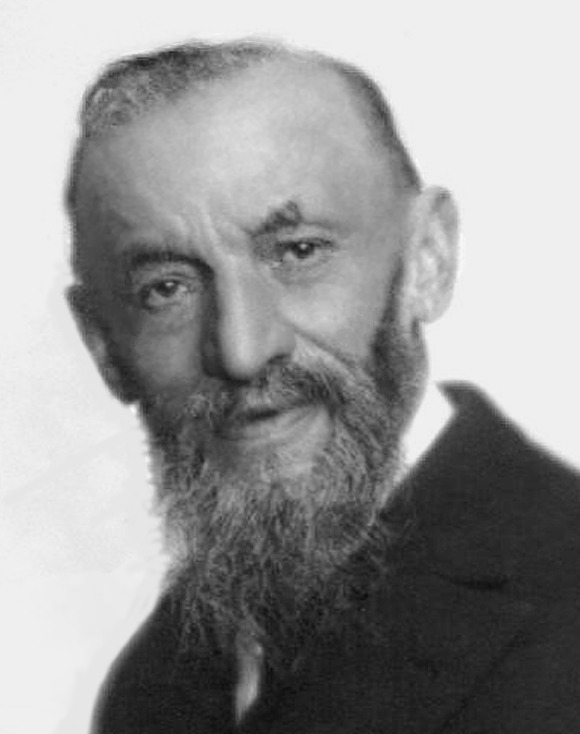
\includegraphics[width=0.5\textwidth]{Peano.jpg}
    \caption{Giuseppe Peano (1858-1932)}
    \label{fig:Peano}
\end{figure}

\begin{aufgabe}{aufgabe:0101}
{Beweisen Sie, dass $2$ eine natürliche Zahl ist. Verwenden Sie dazu lediglich die beiden ersten Peano-Axiome.}
\end{aufgabe}
\noindent
Bereits Giuseppe Peano stellte fest, dass diese ersten beiden Axiome nicht ausreichend sind, um unsere intuitive Vorstellung der natürlichen Zahlen einzufangen. Es könnte sein, dass wir bei dem Vorwärtszählen schliesslich wieder bei $0$ ankommen. Betrachten wir dazu ein Modell der natürlichen Zahlen, welches von $3$ zurück zur $0$ zählt, genauer: $\nu(0)$ ist $1$, $\nu(1)$ ist 2, $\nu(2)$ ist $3$, aber $\nu(3)$ ist wieder $0$ (und gemäss der Definition von $4$ auch gleich der $4$). So erfüllt also auch die Menge $\lrc{0,1,2,3}$ die ersten zwei Peano-Axiome und könnte als Menge der natürlichen Zahlen angesehen werden.
\begin{aufgabe}{aufgabe:0102}
{Welches ist die kleinste Menge, welche die ersten zwei Peano-Axiome erfüllt?}
\end{aufgabe}
\noindent
Die \cref{axiom:a1,axiom:a2} erlauben also auch Mengen, welche wir sicherlich nicht als Modelle der natürlichen Zahlen anschauen möchten. Wir müssen die erlaubten Nachfolger der Elemente der Mengen weiter einschränken. Auf jeden Fall stellen wir fest, dass die $0$ nicht Nachfolger einer natürlichen Zahl sein soll und fordern deshalb:
\axiom{axiom:a3}
{Die $0$ selbst ist nicht der Nachfolger einer natürlichen Zahl.} %Es gilt also $\nu(n)\neq 0$ für jede natürliche Zahl $n$.}

\bemerkung{bemerkung:Nunit}{
Wir bezeichnen mit $\Nunit$ die Menge der natürlichen Zahlen ohne die $0$. Für jede natürliche Zahl $n$ soll der Nachfolger $\nu(n)$ von $n$ wieder eine natürliche Zahl sein. Da gemäss \cref{axiom:a3} die $0$ nicht Nachfolger einer natürlichen Zahl ist, können wir uns $\nu$ als Funktion
\begin{align*}
    \nu: \N&\to\Nunit, \\
    n &\mapsto \nu(n)
\end{align*}
denken. Diese erhält eine natürliche Zahl $n$ als Eingabe und liefert die natürliche Zahl $\nu(n)$, welche nicht die $0$ ist, als Ausgabe.
}
\begin{aufgabe}{aufgabe:0103}
{Beweisen Sie, dass $0\neq 3$ gilt. Verwenden Sie lediglich die ersten drei Peano-Axiome.}
\end{aufgabe}
\noindent
Betrachten Sie ein Zahlensystem, welches $0$ enthält und für das gilt: $\nu(0)$ ist $1$, $\nu(1)$ ist 2, $\nu(2)$ ist $3$, aber $\nu(3)$ bleibt $3$ (also $4=3$, $5=3$, $6=3$ und so weiter). Es ist auch ein Zahlensystem vorstellbar, welches von $3$ zurück zu $1$ geht, also $\nu(3)=1, \nu(1)=2, \nu(2)=3, \nu(3)=1$ und so weiter. Die beiden Beispiele erfüllen alle drei ersten Peano-Axiome. Das Problem ist, dass die ersten drei Peano-Axiome erlauben, dass verschiedene natürliche Zahlen gleiche Nachfolger haben können. Diese Möglichkeit wollen wir also ausschliessen. Dazu fügen wir das vierte Peano-Axiom hinzu:
\axiom{axiom:a4}
{Unterschiedliche natürliche Zahlen haben unterschiedliche Nachfolger. Sind also $n,m$ natürliche Zahlen und $n\neq m$, dann gilt $\nu(n)\neq\nu(m)$. Die Kontraposition dieser Aussage lautet: Gilt $\nu(n)=\nu(m)$, dann folgt $n=m$.}
\begin{aufgabe}{aufgabe:0104}
{Verwenden Sie die ersten vier Peano-Axiome, um zu beweisen, dass $1\neq 4$ gilt.}
\end{aufgabe}
\noindent
Wir wollen $\N$ als die Menge verstehen, welche die $0$ enthält und alle Objekte, welche aus $0$ durch Inkrementieren erhalten werden kann. Diese Intuition wird schliesslich auf geniale Weise durch das fünfte Peano-Axiom formalisiert. Dieses letzte Peano-Axiom formuliert auf mathematisch präzise Weise, was mit \enquote{aus $0$ durch Inkrementieren erhalten werden kann}, gemeint ist:
\axiom{axiom:a5}
{Enthält eine Teilmenge $N\subseteq\N$ das Element $0$ und mit jedem $n\in N$ auch den Nachfolger $\nu(n)$ von $n$, so gilt $N=\N$.}

\subsection{Kompakte Formulierung der Peano-Axiome}\label{subsec:kompakt}
Unser Wissen über Funktionen und ihre Eigenschaften erlaubt uns, die fünf \cref{axiom:a1,axiom:a2,axiom:a3,axiom:a4,axiom:a5}, kompakt und sehr präzise in der folgenden Definition zusammenzufassen:
\begin{definition}[Formale Definition der natürlichen Zahlen]{definition:N}
Die \textbf{natürlichen Zahlen} sind eine Menge $\N$, in der ein Element $0\in\N$ ausgezeichnet ist und für die es eine Funktion $\nu:\N\to\Nunit$ (siehe \cref{bemerkung:Nunit}) mit den folgenden zwei Eigenschaften gibt:
\begin{itemize}
  \item[(N$_0$)] Die Funktion $\nu$ ist injektiv.
  \item[(N$_1$)] Enthält eine Teilmenge $N\subseteq\N$ das Element $0$ und mit jedem $n\in N$ auch den Nachfolger $\nu(n)$ von $n$, so gilt $N=\N$.
\end{itemize}
\end{definition}
Dabei bezeichnet $\Nunit:=\N\setminus{\lrc{0}}$ die Menge der natürlichen Zahlen ohne die $0$. Das Element $\nu(n)$ heisst Nachfolger von $n$ und $\nu$ heisst Nachfolgerfunktion. Die Eigenschaft (N$_1$) ist identisch zum \cref{axiom:a5} und wird auch \tib{Induktionsaxiom}\index{Induktionsaxiom} genannt.
\begin{aufgabe}{aufgabe:0105}
Weisen Sie nach, dass \cref{definition:N} zu den Peano-Axiomen äquivalent ist.
\end{aufgabe}

\begin{aufgabe}{aufgabe:0107}
(*!) Erfüllt auch die Menge $\lrc{0,2,4,6,\ldots}$  der geraden natürlichen Zahlen die Peano-Axiome?
\end{aufgabe}

\begin{aufgabe}{aufgabe:0106}
(*!) Begründen Sie, dass die Nachfolgerfunktion $\nu:\N\to\Nunit$ bijektiv ist.

\noindent
Tipp: Verwenden Sie die beiden Eigenschaften N$_0$ und N$_1$ in \cref{definition:N}.
\end{aufgabe}

\bemerkungen{-}{}
{Aus den grundlegenden Axiomen der Mengenlehre folgt, dass es in der Tat Systeme $(\N,0,\nu)$ gibt, welche die Peano-Axiome erfüllen. Diese Modelle der natürlichen Zahlen sind bis auf die Benennung der Elemente gleichwertig und ergeben dieselbe Mathematik. Beispielsweise könnte man anstelle der arabischen Zahlenschrift auch die römische Zahlenschrift verwenden. Die konkrete Wahl der Symbole ist mathematisch nicht von Bedeutung. Deshalb ist es sinnvoll, von \textit{den} natürlichen Zahlen zu sprechen.}
{Die aus der Schule bekannten Rechenregeln in den natürlichen Zahlen (zum Beispiel das Distributivgesetz) lassen sich allein durch logische Folgerungen aus den Peano-Axiomen beweisen. Diese Beweise werden zum Beispiel in dem Buch \cite{Landau} geführt, welches im Jahr 1930 erschien. Im Vorwort dieses Buchs schreibt der Autor \textit{Edmund Landau} unter anderem:
\begin{itemize}
    \item \enquote{Ich setze nur logisches Denken und die deutsche Sprache als bekannt voraus; nichts aus der Schulmathematik oder gar der höheren Mathematik.}
    \item \enquote{Bitte vergiß alles, was Du auf der Schule gelernt hast; denn Du hast es nicht gelernt.}
\end{itemize}
Wir werden diese (recht umfangreichen) Beweise hier nicht führen. Besonders interessierten Lesenden empfehlen wir in diesem Zusammenhang die entsprechenden Teile in den Büchern \cite{Landau,TerenceTao,AmannEscher1} zu studieren.}

\begin{figure}[H]
    \centering
    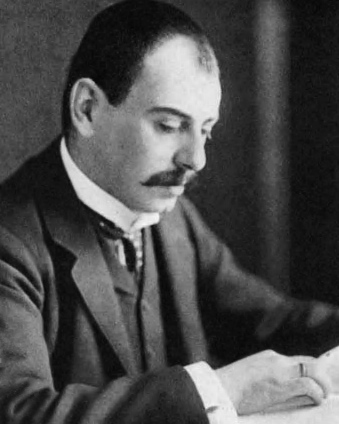
\includegraphics[width=0.4\textwidth]{Landau.jpg}
    \caption{Edmund Landau (1877-1938)}
    \label{fig:Landau}
\end{figure}





\begin{antwort}{aufgabe:0101}
Gemäss \cref{axiom:a1} ist $0$ eine natürliche Zahl. Gemäss \cref{axiom:a2} ist $1=\nu(0)$ eine natürliche Zahl. Schliesslich ist $2=\nu(1)$ wiederum gemäss \cref{axiom:a2} eine natürliche Zahl.
\end{antwort}



\begin{antwort}{aufgabe:0102}
Bereits die Menge $\lrc{0}$ erfüllt die ersten beiden Peano-Axiome. Sie enthält offensichtlich die $0$ und mit $\nu(0):=0$ auch den Nachfolger von jedem $n\in\lrc{0}$ (es gibt nur das eine $n\in\lrc{0}$ und das ist die $0$).
\end{antwort}



\begin{antwort}{aufgabe:0103}
In \cref{aufgabe:0101} haben wir gezeigt, wie aus den ersten zwei Peano-Axiomen folgt, dass $2$ eine natürliche Zahl ist. Definitionsgemäss ist $3=\nu(2)$. Somit ist $3$ der Nachfolger einer natürlichen Zahl und deshalb muss $3$ gemäss dem dritten Peano-Axiom von $0$ verschieden sein, also $0\neq 3$.
\end{antwort}



\begin{antwort}{aufgabe:0104}
Wir beweisen die Aussage durch Widerspruch und nehmen also an, dass $1=4$. Gleichzeitig gilt aber $1=\nu(0)$ und $4=\nu(3)$ und somit $\nu(0)=\nu(3)$. Wegen des vierten Peano-Axioms folgt also $0=3$. Doch in \cref{aufgabe:0103} haben wir gezeigt, dass $0\neq 3$ gilt. Wir haben also einen Widerspruch gefunden und somit muss $1\neq 4$ gelten.
\end{antwort}



\begin{antwort}{aufgabe:0105}
Wir zeigen zuerst, dass \cref{definition:N} alle fünf Peano-Axiome \enquote{abdeckt}.
\begin{itemize}
    \item[\cref{axiom:a1}:] Dieses Axiom ist erfüllt, da in der Definition gefordert wird, dass ein Element $0$ in $\N$ ausgezeichnet ist.
    \item[\cref{axiom:a2}:] Dieses Axiom ergibt sich dadurch, dass $\nu:\N\to\Nunit$ eine Funktion von den natürlichen Zahlen in eine Teilmenge der natürlichen Zahlen ist. Doch die Elemente einer Teilmenge der natürlichen Zahlen sind offensichtlich ebenfalls natürliche Zahlen.
    \item[\cref{axiom:a3}:] Wegen $\nu:\N\to\Nunit$ liegt die $0$ nicht im Bild der Funktion $\nu$. Somit ist also die $0$ nicht Nachfolger einer natürlichen Zahl und damit ist auch dieses Axiom erfüllt.
    \item[\cref{axiom:a4}:] Dieses Axiom sagt genau, dass die Funktion $\nu$ injektiv ist und entspricht somit exakt der Eigenschaft (N$_0$).
    \item[\cref{axiom:a5}:] Dieses Axiom entspricht exakt der Eigenschaft (N$_1$).
\end{itemize}
Da \cref{definition:N} keine zusätzlichen Forderungen stellt, ist diese Definition tatsächlich äquivalent zu den Peano-Axiomen.
\end{antwort}



\begin{antwort}{aufgabe:0107}
Die Frage der Aufgabenstellung geht an der eigentlichen Aussage der Peano-Axiome vorbei und ist im Grunde bedeutungslos. Die Peano-Axiome verlangen nicht, dass die natürlichen Zahlen genau die Form
\begin{align*}
    \lrc{0,1,2,3,4,\ldots}
\end{align*}
haben. Die konkreten Schriftsymbole, mit denen die natürlichen Zahlen bezeichnet werden, werden von den Peano-Axiomen nicht vorgeschrieben. In der üblichen westlichen Schreibweise wird der Nachfolger der $0$ mit dem Symbol $1$ bezeichnet, der Nachfolger von $1$ mit $2$ und so weiter. Anstelle von der Konvention
\begin{align*}
    1:=\nu(0), 2:=\nu(1)=\nu(\nu(0)), 3:=\nu(2)=\nu(\nu(\nu(0))), \ldots
\end{align*}
könnten wir den Nachfolger der $0$ auch mit $2$ bezeichnen und den Nachfolger der $2$ mit $4$ und so weiter. Offensichtlich ist auch das exakte Symbol der Null bedeutungslos. Anstelle von dem Symbol $0$ könnten wir auch das Symbol \twemoji{city_sunset} für dieses ausgezeichnete Element verwenden. Es ist nicht einfach, sich auf diese abstrakte Ebene zu begeben. Sie müssen sich von den konkret verwendeten Schriftsymbolen lösen und sich stattdessen auf die Bedeutung der verwendeten Symbole fokussieren.
\end{antwort}

\begin{antwort}{aufgabe:0106}
Wie können wir beweisen, dass $\nu$ bijektiv ist? Wir dürfen für den Nachweis lediglich bereits bekannte Tatsachen sowie die Peano-Axiome in \cref{definition:N} verwenden. Sicherlich können wir zunächst einmal feststellen, dass die Funktion $\nu$ wegen der Eigenschaft N$_0$ als injektiv vorausgesetzt ist. Damit ist $\nu$ also injektiv. Für den Nachweis der Bijektivität von $\nu$ müssen wir nur noch seine Surjektivität zeigen.

Möchte man eine Eigenschaft nachweisen, ist es zunächst einmal sinnvoll, aufzuschreiben, was diese Eigenschaft genau bedeutet. Definitionsgemäss ist $\nu:\N\to\Nunit$ genau dann surjektiv, wenn das Bild $\text{im}\lr{\nu}$ der Zielmenge $\Nunit$ entspricht, falls also
\begin{align*}
    \textcolor{DarkGreen}{\text{im}\lr{\nu} = \Nunit}
\end{align*}
gilt. Nun haben wir Eigenschaft N$_0$ in \cref{definition:N} bereits ausgenutzt. Es ist daher naheliegend, Eigenschaft N$_1$ zu betrachten. Da N$_1$ eine Aussage über $\N$ und nicht etwa über $\Nunit$ macht, tun wir uns selbst einen Gefallen, wenn wir anstelle von $\Nunit$ die um das Element $0$ erweiterte \enquote{Hilfsmenge}
\begin{align*}
    N := \text{im}\lr{\nu} \cup \lrc{0}
\end{align*}
betrachten. Wir zeigen nun, dass diese Hilfsmenge $N$ eine Teilmenge von $\N$ ist, welche die Bedingungen in N$_1$ erfüllt. Offensichtlich gelten $N\subseteq \N$ und $0\in N$. Für $n\in N$ gilt $\nu(n)\in\text{im}\lr{\nu}\subseteq N$. Somit liegt für $n\in N$ auch der Nachfolger $\nu(n)$ in der Menge $N$ und damit folgt aus N$_1$, dass $N = \N$ gilt. Wir haben also die Gleichheit
\begin{align*}
    \text{im}\lr{\nu} \cup \lrc{0} = \N
\end{align*}
gezeigt und folgern daraus
\begin{align*}
    \textcolor{DarkGreen}{\text{im}\lr{\nu} = \Nunit}.
\end{align*}
\end{antwort}

\clearpage
\shipoutAnswer % Die natürlichen Zahlen
        \chapter{Das Induktionsprinzip}\label{ch:Kapitel02}

\cref{axiom:a5} wird \tib{Prinzip der vollständigen Induktion}\index{Prinzip der vollständigen Induktion} genannt. Dieses Kapitel wird sich mit diesem wichtigen Prinzip befassen.
Sie werden sehen, welche enorm weitreichenden Konsequenzen das \cref{axiom:a5} (Induktionsaxiom) der natürlichen Zahlen hat. Die Notation dieses Kapitels sowie einige Beweise stammen aus Kapitel 5 in \cite{AmannEscher1}.

\section{Einführende Beispiele}

\subsection{Teilbarkeit durch 2}
Ihre gute Freundin Anika behauptet, eine mathematische Entdeckung gemacht zu haben. Sie hat nämlich bemerkt, dass wenn zu dem Quadrat $n^2$ einer natürlichen Zahl $n$ die Zahl $n$ addiert wird, die entstandene Summe stets gerade ist. Sie behauptet also, dass für jede natürliche Zahl $n$ die Zahl $n^2+n$ gerade ist.

\begin{aufgabe}{aufgabe:0200}
Anika hat in der Vergangenheit schon öfters mathematische Behauptungen aufgestellt. Nicht selten haben sich diese bei genauerer Untersuchung als falsch erwiesen. Bevor Sie also viel Zeit in die genauere Analyse Anikas neuer Behauptung investieren, möchten Sie eine kurze \enquote{Plausibilitätsprüfung} durchführen. Schreiben Sie dazu ein Python-Programm, welches für die ersten $100$ natürlichen Zahlen $n\in\setcm{m\in\N}{0\leq m < 100}$ überprüft, ob $n^2+n$ jeweils gerade ist.
\end{aufgabe}
\begin{antwort}{aufgabe:0200}
\begin{lstlisting}[language=Python,caption=Vermutung überprüfen]
def vermutung(m):
    for n in range(m):
        if (n * n + n) % 2 != 0:
            return False
    return True

m = 100
print(vermutung(m))
\end{lstlisting}
\end{antwort}

\noindent
Das folgende Beispiel zeigt in aller Ausführlichkeit, wie das Prinzip der vollständigen Induktion verwendet werden kann, um eine mathematische Vermutung zu beweisen.

\beispiel{beispiel:InduktionEven}
{
Wir betrachten erneut die Vermutung Ihrer Freundin Anika:
\begin{center}
    Für jedes $n\in\N$ ist die Zahl $n^2+n$ gerade.
\end{center}
Wie lässt sich eine solche Vermutung überprüfen? Sicherlich können wir die Vermutung für einige natürliche Zahlen \enquote{von Hand} durch simples \enquote{Nachrechnen} überprüfen. In \cref{aufgabe:0200} haben Sie die Vermutung mit einem Computerprogramm für die ersten 100 natürlichen Zahlen überprüft. Das Problem ist jedoch, dass wir (selbst unter Verwendung von Supercomputern) immer nur endlich viele Zahlen überprüfen können. Wenn wir die Vermutung für 100 Milliarden Zahlen geprüft haben, bleiben immer noch unendlich viele Zahlen, die wir noch nicht betrachtet haben. Was wir benötigen, ist ein mathematisches Argument, welches grundsätzlich erklärt, warum die Vermutung stimmen muss. Ein solches mathematisches Argument liefert uns das Prinzip der vollständigen Induktion. Um dieses direkt anwenden zu können definieren wir die \enquote{Hilfsmenge}
\begin{align*}
    N:=\setct{n\in\N}{$n^2+n$ ist gerade}.
\end{align*}
Die so definierte Menge $N$ enthält genau die natürlichen Zahlen, für welche die Zahl $n^2+n$ gerade ist, für welche also die Vermutung gilt. Somit ist die Vermutung bewiesen, wenn wir nachweisen können, dass alle natürlichen Zahlen in $N$ liegen, dass also die Gleichheit $N=\N$ gilt. Es gilt somit:
\begin{center}
    (für jedes $n\in\N$ ist die Zahl $n^2+n$ gerade) $\quad\iff\quad$ ($N = \N$).
\end{center}
Nun besagt das Prinzip der vollständigen Induktion (\cref{axiom:a5}), dass für eine Teilmenge $N\subseteq\N$ tatsächlich $N=\N$ gilt, falls zwei Bedingungen erfüllt sind:
\begin{enumerate}
    \item $0\in N$,
    \item ist $n\in N$, dann enthält $N$ auch den Nachfolger $\nu(n) = n+1$.
\end{enumerate}
Wir prüfen diese beiden Bedingungen separat:
\begin{enumerate}
    \item In der Tat gilt $0\in N$, denn $0^2+0 = 0$ und $0$ ist gerade. \checkmark
    \item Sei $n\in N$ und somit $\textcolor{Green}{n^2+n}$ eine gerade Zahl. Wir müssen beweisen, dass auch $\nu(n)=(n+1)\in N$ gilt, dass also auch $(n+1)^2+(n+1)$ eine gerade Zahl ist. Dazu betrachten wir die folgende Berechnung:
    \begin{align*}
        (n+1)^2+(n+1) &= n^2+2n+1+(n+1) = n^2+3n+2 =\\
        n^2+n + (2n+2) &= \textcolor{Green}{n^2+n} + 2(n+1).
    \end{align*}
    Betrachten wir den Ausdruck $\textcolor{Green}{n^2+n} + 2(n+1)$. Wir wissen, dass die Zahl $\textcolor{Green}{n^2+n}$ gerade ist (da $n$ in der Menge $N$ liegt). Die Zahl $2(n+1)$ ist offensichtlich ebenfalls gerade. Somit ist $(n+1)^2+(n+1)$ als Summe zweier geraden Zahlen ebenfalls gerade. (Da die Zahl $n^2+n$ gerade ist, existiert eine natürliche Zahl $k$, sodass $n^2+n = 2k$. Dann ist die Summe $(n+1)^2+(n+1) = 2k + 2(n+1) = 2(k+n+1)$ das Doppelte der Zahl $k+n+1$ und somit gerade). \checkmark
\end{enumerate}
Damit sind die Bedingungen des Prinzips der vollständigen Induktion erfüllt und die Gleichheit $N = \N$ (und dadurch die ursprüngliche Vermutung Anikas) bewiesen.
}

\begin{aufgabe}{aufgabe:0299}
Verwenden Sie das Prinzip der vollständigen Induktion um zu beweisen, dass $n^5-n$ für jede natürliche Zahl $n$ durch $5$ teilbar ist.
\end{aufgabe}
\begin{antwort}{aufgabe:0299}
Wir definieren die \enquote{Hilfsmenge}
\begin{align*}
    N:=\setct{n\in\N}{$n^5-n$ ist durch $5$ teilbar}.
\end{align*}
Die Behauptung der Aufgabe ist bewiesen, wenn wir nachweisen können, dass alle natürlichen Zahlen in $N$ liegen, dass also die Gleichheit $N=\N$ gilt. Das Prinzip der vollständigen Induktion (\cref{axiom:a5}) besagt, dass für eine Teilmenge $N\subseteq\N$ tatsächlich $N=\N$ gilt, falls zwei Bedingungen erfüllt sind:
\begin{enumerate}
    \item $0\in N$,
    \item ist $n\in N$, dann enthält $N$ auch den Nachfolger $\nu(n) = n+1$.
\end{enumerate}
Wir prüfen nun diese beiden Bedingungen.
\begin{enumerate}
    \item In der Tat gilt $0\in N$, denn $0^5-0 = 0$ ist durch $5$ teilbar. \checkmark
    \item Sei $n\in N$ und somit $\textcolor{Green}{n^5-n}$ durch $5$ teilbar. Wir müssen beweisen, dass auch $\nu(n)=(n+1)\in N$ gilt, dass also auch $(n+1)^5-(n+1)$ durch $5$ teilbar ist. Dazu betrachten wir die folgende Berechnung:
    \begin{align*}
        (n+1)^5-(n+1) &= n^5+5n^4+10n^3+10n^2+5n+1-n-1 = \\
        &\lr{\textcolor{Green}{n^5-n}} + 5\lr{n^4+2n^3+2n^2+n}
    \end{align*}
    Da $n$ in der Menge $N$ liegt, ist die Zahl $\textcolor{Green}{n^5-n}$ durch $5$ teilbar. Somit ist $(n+1)^5-(n+1)$ als Summe zweier durch $5$ teilbarer Zahlen ebenfalls durch $5$ teilbar. \checkmark
\end{enumerate}
\end{antwort}

\subsection{Klingende Gläser}
In dem Gasthaus \textit{Inn of the Prancing Pony} stossen $n$ Gäste auf das neue Jahr an. Jede Person stösst mit jeder anderen (nicht mit sich selbst) genau einmal an. Wie viele Male klingen die Gläser (wie viele Male wird angestossen)? Die folgende elegante Überlegung, gibt uns eine Formel um die gesuchte Zahl rasch zu berechnen. Jede der $n$ Personen stösst offensichtlich mit genau $(n-1)$ Personen an (mit allen anderen). Damit klingen die Gläser also $n(n-1)$ mal. Die Formel ist so aber noch nicht richtig, denn wir haben jedes Klingen doppelt gezählt (anstatt nur einfach). Stösst nämlich Person $A$ mit Person $B$ an, dann haben wir dieses Anstossen einmal aus Sicht von $A$ gezählt und nochmal aus Sicht von $B$. Somit müssen wir die gesuchte Zahl $n(n-1)$ noch durch den Faktor 2 teilen. Die gesuchte Zahl ist also $n(n-1)/2$.
\beispiel{beispiel:InduktionGlases}
{
Diese Formel wollen wir nun mit Hilfe des Prinzips der vollständigen Induktion überprüfen. Dazu definieren wir, wie bereits in \cref{beispiel:InduktionEven}, die Behauptung in geeigneter Form. Für jedes $n\in\N$ definieren wir also die Aussage $\mathcal{A}(n)$ als
\begin{align*}
    &\mathcal{A}(n) :\iff \\
    &\text{Stossen $n$ Personen (alle mit allen)) an, klingen die Gläser genau } \frac{n(n-1)}{2} \text{ mal}.
\end{align*}
Um das Prinzip der vollständigen Induktion direkt anwenden zu können definieren wir erneut eine \enquote{Hilfsmenge} $N$ der Form
\begin{align*}
    N := \setct{n\in\N}{$\mathcal{A}(n)$ ist wahr}.
\end{align*}
Somit ist die Vermutung bewiesen, wenn wir nachweisen können, dass alle natürlichen Zahlen in $N$ liegen, dass also die Gleichheit $N=\N$ gilt. Erneut prüfen wir die beiden Bedingungen des Induktionsaxioms separat:
\begin{enumerate}
    \item Die behauptete Formel besagt, dass $n = 0$ Personen genau $0\cdot (0-1) = 0$ mal anstossen. Diese ist offensichtlich korrekt und somit haben wir $0\in N$ begründet. \checkmark
    \item Sei $n\in N$ und somit $\mathcal{A}(n)$ wahr. Wir müssen beweisen, dass auch $\nu(n)=(n+1)\in N$ gilt, dass also bei $(n+1)$ Personen genau $\textcolor{Red}{(n+1)n/2}$ mal die Gläser klingen. 
    
    \noindent
    Dazu stellen wir uns vor, dass erst $n$ Personen im Restaurant sind und diese bereits alle miteinander angestossen haben. Da $\mathcal{A}(n)$ wahr ist, wissen wir also, dass die Gläser bereits genau $\textcolor{Green}{n(n-1)/2}$ mal klangen. Nun kommt eine weitere Person hinzu. Diese Person stösst mit allen $\textcolor{Blue}{n}$ bereits anwesenden an. Damit klingen die Gläser genau $n$ weitere Male und insgesamt also
    \begin{align*}
        \textcolor{Green}{\frac{n(n-1)}{2}} + \textcolor{Blue}{n} = \frac{n(n-1)+2n}{2} = \frac{n(n-1+2)}{2} = \textcolor{Red}{\frac{(n+1)n}{2}}
    \end{align*}
    mal. \checkmark
\end{enumerate}
Somit ist die intuitiv gefundene Formel formal mit Hilfe des Prinzips der vollständigen Induktion nachgewiesen.}

\section{Erklimmen einer Leiter}
In \cref{beispiel:InduktionEven} und dem Beweis von \cref{satz:MinimumN} haben wir das Prinzip der vollständigen Induktion als Beweistechnik verwendet. Dabei haben wir jeweils auf geschickte Weise eine \enquote{Hilfsmenge} $N$ definiert und gezeigt, dass $N$ die Menge aller natürlichen Zahlen $\N$ ist. Nun möchten wir aber mathematische Aussagen beweisen und nicht unbedingt über Mengen sprechen. Deshalb ist es intuitiv einfacher, im Beweisverfahren der vollständigen Induktion, den Begriff der \textit{Menge} durch den Begriff der \textit{Aussage} zu ersetzen. Um dies konkreter zu machen, betrachten wir nochmals \cref{beispiel:InduktionEven}. In dem Beispiel kann man für jedes $n\in\N$ die Aussage $\mathcal{A}(n)$ definieren als
\begin{align*}
    \mathcal{A}(n) :\iff \text{Die Zahl $n^2 + n$ ist gerade}.
\end{align*}
In der Sprache der \textit{Aussagen} erhalten wir das folgende rezeptartige Beweisverfahren:
\begin{myBox}[Beweis durch vollständige Induktion]{mybox:Induktion}
Für jedes $n\in\N$ sei $\mathcal{A}(n)$ eine Aussage. Wir wollen beweisen, dass $\mathcal{A}(n)$ für jedes $n\in\N$ richtig ist. Der Beweis kann mit Hilfe des Prinzips der vollständigen Induktion erbracht werden, indem wie folgt vorgegangen wird:
\begin{aenum}
    \item \textit{Induktionsanfang}: Es wird gezeigt, dass $\mathcal{A}(0)$ richtig ist.
    \item \textit{Induktionsschluss}: Dieser besteht aus zwei Teilen:
        \begin{renum}
            \item \textit{Induktionsvoraussetzung}: Es sei $n$ eine natürliche Zahl und $\mathcal{A}(n)$ sei richtig.
            \item \textit{Induktionsschritt} ($n\to n+1)$: Man zeigt, dass aus der Induktionsvoraussetzung (i), logischen Schlüssen und bereits als wahr erkannter Aussagen die Richtigkeit von $\mathcal{A}(n+1)$ abgeleitet werden kann.
        \end{renum}
\end{aenum}
Damit ist die Richtigkeit von $\mathcal{A}(n)$ für alle $n\in\N$ gezeigt.
\end{myBox}
Beachten Sie, dass das Prinzip der vollständigen Induktion dem \cref{axiom:a5} entspricht und als solches nicht bewiesen werden kann. Was wir aber anbieten können, ist eine Metapher, welche das Prinzip veranschaulicht:
\begin{mdframed}[backgroundcolor=NavajoWhite!30,nobreak=true]\label{mdframed:Metapher}
\textbf{Metapher der Leiter}
\vspace{0.2cm}

\noindent
Die vollständige Induktion beweist, dass wir auf einer Leiter beliebig weit hochsteigen können, indem sie beweist, dass wir den untersten Tritt (Induktionsanfang) erreichen
können und, dass wir von jedem Tritt den nächst höheren erreichen können (Induktionsschluss).
\end{mdframed}

\begin{aufgabe}{aufgabe:0201}
Erklären Sie, wie das rezeptartige Beweisverfahren in \cref{mybox:Induktion} aus \cref{axiom:a5} folgt. Tipp: Definieren Sie die \enquote{Hilfsmenge}
\begin{align*}
    N := \setct{n\in\N}{$\mathcal{A}(n)$ ist richtig}
\end{align*}
aller natürlichen Zahlen, für welche $\mathcal{A}(n)$ richtig ist.
\end{aufgabe}
\begin{antwort}{aufgabe:0201}
Im \textit{Induktionsanfang} (a) wird gezeigt, dass $0\in N$ gilt. Der \textit{Induktionsschluss} liefert schliesslich, dass für $n\in N$ auch $(n+1)\in N$ gilt. Gemäss \cref{axiom:a5} gilt somit $N=\N$. Dies bedeutet aber, dass $\mathcal{A}(n)$ in der Tat für alle $n\in\N$ gilt.
\end{antwort}

\begin{aufgabe}{aufgabe:0202}
Beweisen Sie durch vollständige Induktion, dass für jede natürliche Zahl $n$ die Zahl $5^n-1$ durch $4$ teilbar ist.
\end{aufgabe}
\begin{antwort}{aufgabe:0202}
Für jedes $n\in\N$ definieren wir die Aussage $\mathcal{A}(n)$ als
\begin{align*}
    \mathcal{A}(n) :\iff \text{Die Zahl $5^n-1$ durch $4$ teilbar}.
\end{align*}
\begin{aenum}
    \item \textit{Induktionsanfang}: Wir zeigen, dass $\mathcal{A}(0)$ richtig ist. Dies ist aber klar, denn $5^0-1=0$ und $0$ ist durch $4$ teilbar.
    \item \textit{Induktionsschluss}:
        \begin{renum}
            \item \textit{Induktionsvoraussetzung}: Es sei $n$ eine natürliche Zahl und $\mathcal{A}(n)$ sei richtig. Sei also $5^n-1$ durch $4$ teilbar.
            \item \textit{Induktionsschritt} ($n\to n+1)$: Wir zeigen, dass aus der Induktionsvoraussetzung (i), logischen Schlüssen und bereits als wahr erkannter Aussagen die Richtigkeit von $\mathcal{A}(n+1)$ abgeleitet werden kann. Die Aussage $\mathcal{A}(n+1)$ lautet: $5^{n+1}-1$ ist durch $4$ teilbar. Wir berechnen:
            \begin{align*}
                5^{n+1}-1 = 5\cdot 5^{n}-1 = (4+1)\cdot 5^n - 1 = 4\cdot 5^n + \textcolor{Green}{5^n -1}.
            \end{align*}
            Die Zahl $4\cdot 5^n$ ist als Vielfaches von $4$, offensichtlich durch $4$ teilbar und $\textcolor{Green}{5^n -1}$ ist gemäss Induktionsvoraussetzung durch $4$ teilbar. Somit haben wir gezeigt, dass $5^{n+1}-1$ eine Summe von Termen ist, welche jeweils durch $4$ teilbar sind. Damit ist aber auch $5^{n+1}-1$ durch $4$ teilbar und der Induktionsschritt ist bewiesen.
        \end{renum}
\end{aenum}
Aus dem Induktionsprinzip folgt somit, dass $\mathcal{A}(n)$ für jedes $n\in\N$ korrekt ist.
\end{antwort}


\section{Zwei bedeutende Sätze über natürliche Zahlen (*!)}
Das Prinzip der vollständigen Induktion ist in der Mathematik und Informatik von enormer Bedeutung. Wir wollen in diesem anspruchsvollen Abschnitt noch mehr verdeutlichen, wie weitreichend die Beweiskraft dieses Prinzips ist. Dazu möchten wir zwei bedeutende Sätze der Mathematik besprechen und zeigen, wie diese aus dem Prinzip der vollständigen Induktion folgen.
\subsection{Wohlordnungsprinzip}
Beachten Sie, dass die Menge der ganzen Zahlen $\Z$ kein Minimum (kleinstes Element) besitzt. Zu jeder ganzen Zahl $m$ ist offensichtlich $m-1$ ebenfalls eine ganze Zahl, die (noch) kleiner ist als $m$. Die Teilmenge $\lrc{-3,-1,0,7}$ von $\Z$ hingegen besitzt $-3$ als Minimum.
\begin{definition}[ Minimum]{definition:min}
Es sei $A$ eine nichtleere Menge, in der sich Elemente durch die Relation $\leq$ vergleichen lassen. Ein Element $m\in A$ heisst \tib{Minimum}\index{Minimum} von $A$, falls
\begin{align*}
    m \leq x
\end{align*}
für alle $x\in A$ gilt. Das Minimum einer Menge $A$ muss selbst Element von $A$ sein. Beachten Sie, dass $A$ offensichtlich höchstens ein Minimum enthalten kann. Dieses wird mit $\min(A)$ bezeichnet.
\end{definition}

\begin{aufgabe}{aufgabe:0267}
\begin{aenum}
    \item Welches ist das Minimum von $\N$?
    \item Erklären Sie, warum das halboffene Intervall 
    \begin{align*}
        \ioc{0}{1} := \setcm{x\in\R}{0<x\leq 1}
    \end{align*}
    kein Minimum besitzt.
\end{aenum}
\end{aufgabe}
\begin{antwort}{aufgabe:0267}
    \begin{aenum}
        \item Die Zahl $0$ ist das Minimum von $\N$, da $0\in\N$ und $0\leq x$ für alle $x\in\N$.
        \item Für jedes Element $m\in\ioc{0}{1}$ ist auch die Hälfte $m/2$ von $m$ Element des Intervalls. Dann gilt aber auch $\lr{m/2}\in\ioc{0}{1}$. Anders gesagt: Angenommen $m\in\ioc{0}{1}$ sei das Minimum des Intervalls. Dann gilt aber auch $\lr{m/2}\in\ioc{0}{1}$. Wegen $m/2<m$ ist dies aber ein Widerspruch zur Minimalität von $m$.
    \end{aenum}
\end{antwort}
Wir haben gesehen, dass durchaus nicht jede Menge ein Minimum besitzt. Das sogenannte \tib{Wohlordnungsprinzip}\index{Wohlordnungsprinzip} der natürlichen Zahlen garantiert uns aber, dass jede Teilmenge von $\N$, welche nicht die leere Menge ist, ein Minimum besitzt. Die leere Menge besitzt keine Elemente und somit offensichtlich auch kein minimales Element. Weshalb ist das Wohlordnungsprinzip für uns interessant? Dieses Prinzip kommt in den Beweisen einiger wichtiger mathematischen Behauptungen zum Einsatz. So zum Beispiel in unserem Beweis des berühmten \textit{Fundamentalsatzes der Arithmetik}, den wir in \cref{subsec:fundamental} besprechen.

\begin{definition}[untere Schranke]{definition:schranke}
Seien $D$ eine Menge und $A\subseteq D$ eine nichtleere Teilmenge von $D$. Jedes Element $s\in D$, welches $s \leq a$ für alle $a\in A$ erfüllt, heisst \tib{untere Schranke}\index{untere Schranke} von $A$. Eine untere Schranke von $A$ muss selbst nicht ein Element von $A$ sein.   
\end{definition}
\noindent
Wir erkennen nun: Ein Element $m\in\R$ heisst \textit{Minimum} von $A\in\R$, falls $m$ eine untere Schranke von $A$ ist und zusätzlich $m\in A$ gilt.

\beispiele{-}{}
{Die Zahlen $-5, 0, 3, 4$ sind Beispiele von unteren Schranken der Menge $A:=\lrc{4,7,9,18}$. Da $4\in A$ und $4$ eine untere Schranke von $A$ ist, gilt
\begin{align*}
    \min(A) = 4.
\end{align*}
}
{Die Menge $\Z$ der ganzen Zahlen besitzt keine untere Schranke.}

\begin{aufgabe}{aufgabe:0298}
Welches ist die grösste untere Schranke des halboffenen Intervalls
    \begin{align*}
        \ioc{0}{1} := \setcm{x\in\R}{0<x\leq 1}?
    \end{align*}
\end{aufgabe}
\begin{antwort}{aufgabe:0298}
Das halboffene Intervall $\ioc{0}{1} := \setcm{x\in\R}{0<x\leq 1}$ besitzt die grösste untere Schranke $0$, aber kein Minimum.
\end{antwort}

\begin{aufgabe}{aufgabe:0297}
    \begin{aenum}
        \item Sei $A\subseteq\N$ eine Teilmenge der natürlichen Zahlen. Angenommen $n\in\N$ sei eine untere Schranke von $A$, wobei aber $n$ selbst nicht Element der Menge $A$ ist ($n$ ist also nicht das Minimum von $A$). Begründen Sie, warum auch der Nachfolger $n+1$ eine untere Schranke von $A$ ist.
        \item Sei $A\subseteq\N$ eine Teilmenge der natürlichen Zahlen mit der Eigenschaft, dass jede natürliche Zahl eine untere Schranke von $A$ ist. Beweisen Sie, dass $A$ die leere Menge ist. Tipp: Nehmen Sie an, $A$ sei nichtleer. Dann enthält $A$ also (zumindest) ein Element $m\in A$. Betrachten Sie nun die natürliche Zahl $m+1$.
    \end{aenum}
    \end{aufgabe}
    \begin{antwort}{aufgabe:0297}
    \begin{aenum}
        \item Da $n$ eine untere Schranke von $A$ ist, gilt $n\leq a$ für alle $a\in A$. Da aber $n\notin A$, ist klar, dass tatsächlich sogar $n < a$ (echt kleiner) für alle $a\in A$ gilt. Der Nachfolger (die nächst grössere natürliche Zahl) von $n$ ist $n+1$. Damit ist klar, dass $n+1$ höchstens so gross wie jedes der Elemente in $A$ ist, dass also $n+1 \leq a$ für alle $a\in A$ gilt.
        \item Angenommen $A$ wäre nichtleer. Dann enthält $A$ mindestens ein Element $m\in A$. Die natürliche Zahl $m+1$ ist grösser als $m\in A$ und somit keine untere Schranke von $A$. Doch $A$ besitzt die Eigenschaft, dass jede natürliche Zahl eine untere Schranke von $A$ ist. Dies ist ein Widerspruch und somit muss $A$ die leere Menge sein.
    \end{aenum}
\end{antwort}

\noindent
Wir verwenden nun das Prinzip der vollständigen Induktion, um das \textit{Wohlordnungsprinzip} zu beweisen. Wir haben den Beweis dieses Satzes inzwischen recht gut vorbereitet. Dennoch ist der Beweis recht anspruchsvoll! Nehmen Sie sich Zeit um die einzelnen Schritte zu studieren.
\begin{satz}[Wohlordnungsprinzip]{satz:MinimumN}
{Jede nichtleere Teilmenge der natürlichen Zahlen besitzt ein Minimum.}
\end{satz}
\beweis{
Wir beweisen den Satz durch Widerspruch. Angenommen eine Teilmenge $A\subseteq\N$ sei \textbf{nichtleer} und besitze \textbf{kein Minimum}. Dann definieren wir zu $A$ die \enquote{Hilfsmenge}
\begin{align*}
    N := \setct{n\in\N}{$n$ ist untere Schranke von $A$}
\end{align*}
aller unteren Schranken von $A$. Mit dem Prinzip der vollständigen Induktion beweisen wir, dass jede natürliche Zahl eine untere Schranke von $A$ ist, dass also $N=\N$ gilt. In \cref{aufgabe:0298} haben Sie bereits bewiesen, dass dies nur möglich ist, falls $A$ die leere Menge ist. Um $N = \N$ durch die vollständige Induktion zu beweisen, müssen wir, wie immer, zwei Bedingungen prüfen:
\begin{enumerate}
    \item $0\in N$,
    \item Ist $n\in N$, dann enthält $N$ auch den Nachfolger $\nu(n) = n+1$ von $n$. \textcolor{Gray}{(Ist $n$ eine untere Schranke von $A$, dann ist auch $n+1$ eine untere Schranke von $A$.)}
\end{enumerate}
Wir prüfen diese beiden Bedingungen separat:
\begin{enumerate}
    \item $0$ ist die kleinste Zahl in $\N$ und somit gilt $0\leq a$ für jedes Element $a\in A$. Damit ist $0$ eine untere Schranke von $A$ und wir haben $0\in N$ gezeigt. \checkmark
    \item Es sei $n\in N$ und somit $n$ eine untere Schranke von $A$. Beachten Sie, dass $n$ nicht in $A$ liegt, denn sonst würde die Menge $A$ die Zahl $n$ als ihr Minimum besitzen (doch $A$ besitzt gemäss Annahme kein Minimum). Damit ist $n\in\N$ eine untere Schranke von $A$, wobei aber $n$ selbst nicht Element der Menge $A$ ist. In \cref{aufgabe:0297} haben Sie gezeigt, dass dann auch $n+1$ eine untere Schranke von $A$ und somit ein Element von $N$ ist. \checkmark
\end{enumerate}
Aus dem Prinzip der vollständigen Induktion folgt nun, dass $N=\N$ gilt. Also ist jede natürliche Zahl eine untere Schranke von $A$. Somit ist $A\subseteq\N$ eine Teilmenge der natürlichen Zahlen mit der Eigenschaft, dass jede natürliche Zahl eine untere Schranke von $A$ ist. In \cref{aufgabe:0297} haben Sie gezeigt, dass $A$ somit die leere Menge ist. Damit haben wir den gewünschten Widerspruch $A\neq\emptyset$ und $A=\emptyset$ gefunden. Somit besitzt jede nichtleere Teilmenge von $\N$ ein Minimum.}

\subsection{Fundamentalsatz der Arithmetik}\label{subsec:fundamental}
Die Tatsache, dass jede Teilmenge der natürlichen Zahlen ein Minimum besitzt, erlaubt uns, den berühmten \textit{Fundamentalsatz der Arithmetik} zu beweisen.
\begin{satz}[Fundamentalsatz der Arithmetik (Primfaktorzerlegung)]{satz:Fundamentalsatz}
Ausser $0$ und $1$ kann jede natürliche Zahl als Produkt endlich vieler Primzahlen dargestellt werden. Diese Darstellung ist bis auf die Reihenfolge der Faktoren eindeutig und wird \textit{Primfaktorzerlegung} genannt. Erlaubt sind auch Produkte, die nur aus einem Faktor bestehen.
\end{satz}
\beispiele{-}{}
{Die Zahl $63$ besitzt die Primfaktorzerlegung $63 = 3\cdot 3\cdot 7$ und die Zahl $286$ die Darstellung $286 = 2\cdot 11\cdot 13$.}
{Die Primfaktorzerlegung der Primzahl $19$ ist $19$ selbst. Sie besteht also aus dem Produkt mit nur dem einen Faktor $19$. Jede Primzahl $p$ ist also bereits in Primfaktoren zerlegt.}

\beweis{Wir wollen nun den Fundamentalsatz (\cref{satz:Fundamentalsatz}) beweisen. Dies tun wir unter der Verwendung des Wohlordnungsprinzips. Allerdings zeigen wir nur, dass immer eine Zerlegung in Primfaktoren existiert. Auf den Beweis der Eindeutigkeit verzichten wir an dieser Stelle.

Angenommen die Behauptung sei falsch. Dann gibt es eine natürliche Zahl $\geq 2$, welche keine Primfaktorzerlegung besitzt. Mit anderen Worten: Die Menge
\begin{align*}
    A := \setct{n\in\N}{$n\geq 2$ und $n$ besitzt keine Primfaktorzerlegung}
\end{align*}
ist \textbf{nichtleer}. Dann liegt in $A$ aber gemäss \cref{satz:MinimumN} eine kleinste Zahl $n_0\geq 2$, welche nicht in Primfaktoren zerlegt werden kann. Insbesondere ist $n_0$ keine Primzahl. Da $n_0$ keine Primzahl ist, existieren natürliche Zahlen $n$ und $m$, sodass $n_0=n\cdot m$ und $n,m>1$. Es ist klar, dass die Faktoren $n$ und $m$ jeweils kleiner als das Produkt $n_0$ sind. Da aber $n_0$ die kleinste natürliche Zahl ist, welche keine Primfaktorzerlegung besitzt, können sowohl $n$ als auch $m$ jeweils als Produkt endlich vieler Primzahlen geschrieben werden. Dann ist aber auch $n_0$ als Produkt von $n$ und $m$ ein Produkt endlich vieler Primzahlen. Dieses Produkt wäre denn aber eine Primfaktorzerlegung von $n_0$. Das ist ein Widerspruch.}


\begin{aufgabe}{aufgabe:0293}
Die Zahl $30031$ lässt sich als Produkt
\begin{align*}
    30031 = p_1p_2
\end{align*}
zweier verschiedener Primfaktoren $p_1$ und $p_2$ schreiben. Schreiben Sie ein Python-Programm, welches $p_1$ und $p_2$ berechnet.
\end{aufgabe}
\begin{antwort}{aufgabe:0293}
\begin{lstlisting}[language=Python]
n = 30031
for k in range(2,n):
    if (n % k == 0):
        p1 = k
        break
p2 = int(n / p1)
print(n,'=', p1, '*',p2)
\end{lstlisting}
\end{antwort}


\begin{aufgabe}{aufgabe:0292}
Der griechische Mathematiker \textit{Euklid von Alexandria} bewies bereits im 3. Jahrhundert v. Chr., dass unendlich viele Primzahlen existieren. Dazu nahm er (indirekter Beweis) an, die Menge $P$ aller Primzahlen sei endlich. Wir können $P$ also schreiben als
\begin{align*}
    P = \lrc{p_1, p_2, p_3, \ldots , p_n}.
\end{align*}
Nun betrachtete Euklid das Produkt dieser $n$ Primzahlen und addierte dazu $1$:
\begin{align*}
    m := p_1\cdot p_2\cdot p_3\cdot \ldots \cdot p_n + 1.
\end{align*}
Betrachten Sie die so entstandene Zahl $m$. Welche Eigenschaften hat $m$ gemäss unseren Annahmen? Vervollständigen Sie den Beweis.
\end{aufgabe}
\begin{antwort}{aufgabe:0292}
Da $m\geq 2$ ist, lässt sich $m$ gemäss \cref{satz:Fundamentalsatz} als Produkt von Primzahlen schreiben. Für jeden Primteiler $p$ von $m$ gilt $p\neq p_i$ für alle $i=1,2,\ldots , n$. Es gibt also eine weitere Primzahl $p\notin P$. Dies ist ein Widerspruch zur Annahme, dass $P$ alle Primzahlen enthält.
\end{antwort}

\bemerkung{-}{Beachten Sie, dass das Vorgehen in \cref{aufgabe:0292} in keinster Weise ein Rezept zur Konstruktion von Primzahlen liefert. Beispielsweise gilt
\begin{align*}
    2\cdot 3\cdot 5\cdot 7\cdot 11\cdot 13 + 1 = 30031,
\end{align*}
doch Sie haben in \cref{aufgabe:0293} bereits gezeigt, dass $30031$ keine Primzahl ist.
}

\clearpage
\section{Leicht verallgemeinertes Induktionsprinzip}
Wie Sie sofort nachprüfen können, ist die mathematische Aussage $n^2 - 2n - 1 > 0$ für die natürlichen Zahlen $n = 0, 1, 2$ falsch. Nun möchten Sie aber beweisen, dass die Aussage für alle $n\in\N$ mit $n\geq 3$ gilt. Unser Beweisverfahren in \cref{mybox:Induktion} muss also dahingehend angepasst werden, dass es uns auch erlaubt, den Induktionsanfang bei einer beliebigen Zahl $n_0\in\N$ anzusetzen, wobei $n_0$ auch grösser als $0$ sein darf. Diese sehr geringfügige (aber wichtige) Verallgemeinerung fassen wir in dem folgenden Satz zusammen:
\begin{satz}[(leicht verallgemeinertes) Induktionsprinzip]{satz:n0Induktion}
Sei $n_0\in\N$ und für jedes $n\in\N$ mit $n\geq n_0$ sei $\mathcal{A}(n)$ eine Aussage. Zudem gelte:
\begin{renum}
    \item $\mathcal{A}\lr{n_0}$ ist richtig.
    \item Für jede Zahl $n\in\N$ mit $n\geq n_0$ folgt aus der Richtigkeit von $\mathcal{A}(n)$ die Richtigkeit von $\mathcal{A}(n+1)$.
\end{renum}
Dann ist $\mathcal{A}(n)$ für jedes $n\geq n_0$ richtig.
\end{satz}
\beweis{Der Beweis ist fast komplett analog zu der Begründung in \cref{aufgabe:0201}. Der einzige Unterschied besteht darin, dass wir einen Index \enquote{verschieben} müssen. Intuitiv gesprochen, möchten wir, dass wir immer noch bei $0$ beginnen, anstelle von $\mathcal{A}(0)$ aber bereits $\mathcal{A}\lr{n_0}$ betrachten. Wir definieren also die Menge $N$ der um \enquote{$\textcolor{Red}{n_0}$ verschobenen Aussagen}
\begin{align*}
    N := \setct{n\in\N}{$\mathcal{A}\lr{n+\textcolor{Red}{n_0}}$ ist richtig}.
\end{align*}
Beachten Sie, dass für $n=0$ dadurch bereits die Aussage $\mathcal{A}\lr{0+n_0}=\mathcal{A}\lr{n_0}$ gemeint ist. Mit dem Induktionsaxiom \ref{axiom:a5} folgt sofort $N=\N$ und somit ist $\mathcal{A}(n)$ für jedes $n\geq n_0$ richtig.}

\bemerkung{-}{
Wir werden das leicht verallgemeinerte Induktionsprinzip von \cref{satz:n0Induktion} ebenfalls einfach nur \textit{Induktionsprinzip} nennen.
}

\section{Übungsaufgaben zum Induktionsprinzip}

\begin{aufgabe}{aufgabe:0204}
Setzen Sie $n_0 := 3$ und beweisen Sie die Korrektheit der Ungleichung $n^2 - 2n - 1 > 0$ für alle $n\in\N$ mit $n\geq n_0$ mittels vollständiger Induktion.
\end{aufgabe}

\begin{antwort}{aufgabe:0204}
Für jedes $n\in\N$ mit $n\geq n_0$ definieren wir die Aussage $\mathcal{A}(n)$ als
\begin{align*}
    \mathcal{A}(n) :\iff n^2-2n-1 > 0.
\end{align*}
\begin{aenum}
    \item \textit{Induktionsanfang}: Wir zeigen, dass $\mathcal{A}(n_0)$ richtig ist. Für $n=3$ ist
    \begin{align*}
        n^2-2n-1 = 9-6-1 = 2 > 0.
    \end{align*}
    Somit stimmt die Aussage für $n=3$.
    \item \textit{Induktionsschluss}:
        \begin{renum}
            \item \textit{Induktionsvoraussetzung}: Es sei $n\geq n_0$ eine natürliche Zahl und $\mathcal{A}(n)$ sei richtig. Sei also
            \begin{align*}
                \textcolor{Green}{n^2-2n-1} > 0.
            \end{align*}
            \item \textit{Induktionsschritt} ($n\to n+1)$: Wir schreiben die Aussage $\mathcal{A}(n+1)$ explizit hin:
            \begin{align*}
                \textcolor{Red}{(n+1)^2-2(n+1)-1} > \textcolor{Red}{0}.
            \end{align*}
            Beweis des Induktionsschritts:
            \begin{align*}
                &\textcolor{Red}{(n+1)^2-2(n+1)-1} = n^2 + 2n + 1 - 2n - 2 - 1 = \\
                &\textcolor{Green}{n^2-2n-1} + 2n+1-2 = \textcolor{Green}{n^2-2n-1} + 2n-1 \stackrel{\text{Induktionsvoraussetzung}}{>}\\
                &2n-1 > \textcolor{Red}{0}.
            \end{align*}
        Beachten Sie, dass für $n\geq 0$ der Term $2n-1$ grösser als $0$ ist.
        \end{renum}
\end{aenum}
Mit \cref{satz:n0Induktion} folgt, dass $\mathcal{A}(n)$ für jedes $n\in\N$ mit $n\geq 3$ korrekt ist.
\end{antwort}

\begin{aufgabe}{aufgabe:0205}
Sie vermuten, dass die Zahl $n^3-n$ für jede natürliche Zahl $n\geq 2$ durch $3$ teilbar ist. Beweisen Sie diese Behauptung durch vollständige Induktion. Finden Sie auch einen direkten Beweis (welcher nicht das Induktionsprinzip verwendet)? Tipp für den direkten Beweis: Schreiben Sie die Zahl $n^3-n$ als Produkt dreier Faktoren.
\end{aufgabe}

\begin{antwort}{aufgabe:0205}
Die Behauptung lässt sich sehr elegant direkt beweisen, wenn man die Zahl $n^3-n$ als das Produkt
\begin{align*}
    n^3-n = (n-1)n(n+1)
\end{align*}
von drei Faktoren schreibt. Da die drei Zahlen $(n-1), n$ und $(n+1)$ direkt aufeinander folgen, muss genau eine von ihnen durch $3$ teilbar sein. Damit besitzt aber mindestens ein Faktor den Teiler $3$. Somit ist das Produkt $(n-1)n(n+1)$ und dadurch auch $n^3-n$ durch $3$ teilbar. Dies stellt einen direkten Beweis der Aussage dar.

Nun beweisen wir die Aussage auch durch vollständige Induktion. Für jedes $n\in\N$ mit $n\geq 2$ definieren wir die Aussage $\mathcal{A}(n)$ als
\begin{align*}
    \mathcal{A}(n) :\iff \text{Die Zahl } n^3-n \text{ ist durch $3$ teilbar}.
\end{align*}
\begin{aenum}
    \item \textit{Induktionsanfang}: Wir zeigen, dass $\mathcal{A}(2)$ richtig ist. Für $n=2$ ist
    \begin{align*}
        n^3-n = 2^3-2 = 6
    \end{align*}
    und $6$ ist durch $3$ teilbar. Somit stimmt die Aussage für $n=2$.
    \item \textit{Induktionsschluss}:
        \begin{renum}
            \item \textit{Induktionsvoraussetzung}: Es sei $n\geq n_0$ eine natürliche Zahl und $\mathcal{A}(n)$ sei richtig. Sei also $\textcolor{Green}{n^3-n}$ durch $3$ teilbar.
            \item \textit{Induktionsschritt} ($n\to n+1)$:
            \begin{align*}
                & (n+1)^3-(n+1) = \\
                & n^3+3n^2+3n+1 - (n+1) = \\
                & n^3+3n^2+2n = \\
                & n^3-n+3n^2+3n = \\
                & \underbrace{\textcolor{Green}{n^3-n}}_{\text{Induktionsvoraussetzung}}+\underbrace{3(n^2+n)}_{\text{ganzzahliges Vielfaches von $3$}}
            \end{align*}
        Der erste Summand ist nach Induktionsvoraussetzung durch $3$ teilbar. Der zweite Summand ist als ganzzahliges Vielfaches von $3$ ebenfalls durch $3$ teilbar. Damit ist die Aussage auch für $n+1$ erfüllt.
        \end{renum}
\end{aenum}
Mit \cref{satz:n0Induktion} folgt, dass $\mathcal{A}(n)$ für jedes $n\in\N$ mit $n\geq 2$ korrekt ist.
\end{antwort}

\begin{aufgabe}[Bernoullische Ungleichung]{aufgabe:0206}
Es sei $x\in\R$ mit $x\geq -1$ eine reelle Zahl. Für jede natürliche Zahl $n$ gilt die Bernoullische Ungleichung $(1+x)^n\geq 1+nx$.
\begin{figure}[H]
    \centering
    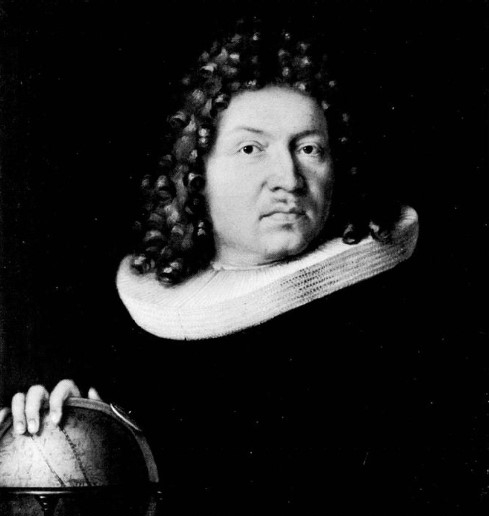
\includegraphics[width=0.20\textwidth]{Bernoulli.jpg}
    \caption{Jakob I Bernoulli (1654-1705) war ein Schweizer Mathematiker und Mitglied der angesehenen Gelehrtenfamilie Bernoulli.}
    \label{fig:Bernoulli}
\end{figure}
\end{aufgabe}
\begin{antwort}{aufgabe:0206}
Es sei $x\in\R$ mit $x\geq -1$ eine reelle Zahl. Für jedes $n\in\N$ definieren wir die Aussage $\mathcal{A}(n)$ als
\begin{align*}
    \mathcal{A}(n) :\iff (1+x)^n\geq 1+nx.
\end{align*}
\begin{aenum}
    \item \textit{Induktionsanfang}: Wir zeigen, dass $\mathcal{A}(0)$ richtig ist. Für $n=0$ ist
    \begin{align*}
        (1+x)^0 = 1 \geq 1 + 0\cdot x = 1.
    \end{align*}
    Somit stimmt die Aussage für $n=0$.
    \item \textit{Induktionsschluss}:
        \begin{renum}
            \item \textit{Induktionsvoraussetzung}: Es sei $n\geq n_0$ eine natürliche Zahl und $\mathcal{A}(n)$ sei richtig. Sei also
            \begin{align*}
                \textcolor{Green}{(1+x)^n} \geq \textcolor{Blue}{1+nx}.
            \end{align*}
            \item \textit{Induktionsschritt} ($n\to n+1)$: Wir schreiben die Aussage $\mathcal{A}(n+1)$ explizit hin:
            \begin{align*}
                \textcolor{Red}{(1+x)^{n+1}} \geq \textcolor{Red}{1 + (n+1)x}.
            \end{align*}
            Beweis des Induktionsschritts:
            \begin{align*}
                &\textcolor{Red}{(1+x)^{n+1}} = \textcolor{Green}{(1+x)^n} (1+x) \stackrel{\text{Induktionsvoraussetzung und }(1+x)\geq 0}{\geq}\\
                &\textcolor{Blue}{(1+nx)}(1+x) = 1+x+nx+nx^2 = 1+(n+1)x + nx^2 \stackrel{(nx^2)\geq 0}{\geq}\\
                &\textcolor{Red}{1 + (n+1)x}.
            \end{align*}
        Doch dies ist genau die Behauptung $\mathcal{A}(n+1)$.
        \end{renum}
\end{aenum}
Aus dem Induktionsprinzip folgt somit, dass $\mathcal{A}(n)$ für jedes $n\in\N$ korrekt ist.
\end{antwort}

\begin{aufgabe}{aufgabe:0207}
(*!) In die Ebene wurden $n\in\N$ verschiedene Geraden gelegt. Die Geraden teilen die Ebene in verschiedene Bereiche. Wir sagen, dass zwei Bereiche \textit{benachbart} sind, falls sie sich eine (möglicherweise unendlich lange) Grenzlinie teilen. Falls zwei Bereiche lediglich einen Grenzpunkt teilen (keine Grenzlinie), sind sie nicht benachbart.

Wir haben zwei Farben zur Verfügung und müssen jeden Bereich mit genau einer dieser Farben einfärben. Eine Färbung wird \textit{zulässig} genannt, falls zusätzlich keine zwei benachbarten Bereiche mit derselben Farbe gefärbt wurden. In \cref{fig:2lines} ist eine mögliche zulässige Färbung für zwei Geraden ($n=2$) gezeigt.

Skizzieren Sie eine zulässige Färbung für $n=3$ für den Fall, dass sich alle drei Geraden jeweils gegenseitig schneiden. Beweisen Sie anschliessend durch vollständige Induktion, dass es immer möglich ist, die verschiedenen Bereiche mit nur zwei Farben so zu färben, dass keine zwei benachbarten Bereiche von derselben Farbe sind.

% 2 lines
\begin{figure}[H]
    \centering
    \begin{subfigure}{0.4\textwidth}
        \centering
        \begin{tikzpicture}[scale=0.50]
            \colorlet{c1}{Gold}
            \colorlet{c2}{CornflowerBlue}
    
            \coordinate (A1) at (-4,-2);
            \coordinate (A2) at (4,2);
            \coordinate (B1) at (-4,2);
            \coordinate (B2) at (4,-2);
            
            \node[below left] at (A1) {$g_1$};
            \node[above left] at (B1) {$g_2$};
            
            \foreach \k in {A,B}
                \draw[black, thick] (\k1) -- (\k2);
        \end{tikzpicture}
        \caption{zwei sich schneidende Geraden}
        \label{subfig:2linesNotFilled}
    \end{subfigure}
    \hfill
    \begin{subfigure}{0.4\textwidth}
        \centering
        \begin{tikzpicture}[scale=0.50]
            \colorlet{c1}{Gold}
            \colorlet{c2}{CornflowerBlue}
    
            \coordinate (A1) at (-4,-2);
            \coordinate (A2) at (4,2);
            \coordinate (B1) at (-4,2);
            \coordinate (B2) at (4,-2);
            
            \node[below left] at (A1) {$g_1$};
            \node[above left] at (B1) {$g_2$};
            
            \coordinate (X) at (intersection cs:first line={(A1)--(A2)}, second line={(B1)--(B2)});
            
            \fill[c1,opacity=0.7]
                (A1) -- (X) -- (B2);
            \fill[c1,opacity=0.7]
                (B1) -- (X) -- (A2);
            \fill[c2,opacity=0.7]
                (A1) -- (X) -- (B1);
            \fill[c2,opacity=0.7]
                (A2) -- (X) -- (B2);
            \foreach \k in {A,B}
                \draw[black, thick] (\k1) -- (\k2);
        \end{tikzpicture}
        \caption{zulässige Färbung für $n=2$}
        \label{subfig:2linesFilled}
    \end{subfigure}
    \caption{Beispiel einer zulässigen Färbung für $n=2$. Beachten Sie, dass die beiden \textcolor{Gold}{goldenen} Bereiche sich nur einen Grenzpunkt (keine Grenzlinie) teilen und somit nicht benachbart sind. Das Gleiche gilt für die beiden \textcolor{CornflowerBlue}{blauen} Bereiche. Zwei sich schneidende Geraden teilen die Ebene in vier Bereiche ein. Zwei parallele Geraden teilen die Ebene in drei Bereiche ein.}
    \label{fig:2lines}
\end{figure}
\end{aufgabe}

\begin{antwort}{aufgabe:0207}
In \cref{fig:3lines} ist eine zulässige Färbung für drei Geraden skizziert.
% 3 lines
\begin{figure}[H]
    \centering
     \begin{subfigure}[b]{0.45\textwidth}
        \centering
        \begin{tikzpicture}[scale=0.7]
            \colorlet{c1}{Gold}
            \colorlet{c2}{CornflowerBlue}
            
            \coordinate (A1) at (-2,-2);
            \coordinate (A2) at (2,3);
            \coordinate (B1) at (-3,0);
            \coordinate (B2) at (5,0);
            \coordinate (C1) at (-1,3);
            \coordinate (C2) at (5,-2);
            
            \node[below left] at (A1) {$g_1$};
            \node[left] at (B1) {$g_2$};
            \node[above left] at (C1) {$g_3$};
            
            \foreach \k in {A,B,C}
                \draw[black, thick] (\k1) -- (\k2);
        \end{tikzpicture}
        \caption{Drei verschiedene Geraden $g_1, g_2$ und $g_3$ teilen die Ebene in sieben Bereiche ein.}
        \label{subfig:3linesNotFilled}
    \end{subfigure}
    \begin{subfigure}[b]{0.45\textwidth}
        \centering
        \begin{tikzpicture}[scale=0.7]
            \colorlet{c1}{Gold}
            \colorlet{c2}{CornflowerBlue}
            
            \coordinate (A1) at (-2,-2);
            \coordinate (A2) at (2,3);
            \coordinate (B1) at (-3,0);
            \coordinate (B2) at (5,0);
            \coordinate (C1) at (-1,3);
            \coordinate (C2) at (5,-2);
            
            \node[below left] at (A1) {$g_1$};
            \node[left] at (B1) {$g_2$};
            \node[above left] at (C1) {$g_3$};
            
            \coordinate (X) at (intersection cs:first line={(A1)--(A2)}, second line={(B1)--(B2)});
            \coordinate (Y) at (intersection cs:first line={(A1)--(A2)}, second line={(C1)--(C2)});
            \coordinate (Z) at (intersection cs:first line={(B1)--(B2)}, second line={(C1)--(C2)});
            
            \fill[c1,opacity=0.7]
                (A1) -- (X) -- (B1);
            \fill[c1,opacity=0.7]
                (A2) -- (Y) -- (C1);
            \fill[c1,opacity=0.7]
                (B2) -- (Z) -- (C2);
            \fill[c1,opacity=0.7]
                (X) -- (Y) -- (Z);
        
            \fill[c2,opacity=0.7]
                (A1) -- (X) -- (Z) -- (C2);
            \fill[c2,opacity=0.7]
                (B1) -- (X) -- (Y) -- (C1);
            \fill[c2,opacity=0.7]
                (A2) -- (Y) --(Z) -- (B2);
            
            \foreach \k in {A,B,C}
                \draw[black, thick] (\k1) -- (\k2);
        \end{tikzpicture}
        \caption{zulässige Färbung für $n=3$}
        \label{subfig:3linesFilled}
    \end{subfigure}
    \caption{zulässige Färbung für drei Geraden}
    \label{fig:3lines}
\end{figure}
\noindent
Für jedes $n\in\N$ definieren wir die Aussage $\mathcal{A}(n)$ als
\begin{center}
    $\mathcal{A}(n) :\iff $ Die Bereiche, welche durch $n$ verschiedene Geraden in der Ebene geformt werden, besitzen eine zulässige Färbung.
\end{center}
\begin{aenum}
    \item \textit{Induktionsanfang}: Wir zeigen, dass $\mathcal{A}(0)$ richtig ist. Für $n=0$ haben wir gar keine Gerade und nur einen einzigen Bereich (nämlich die gesamte Ebene). Dieser Bereich kann entweder golden oder blau gefärbt werden, um eine zulässige Färbung zu erhalten.
    \item \textit{Induktionsschluss}:
        \begin{renum}
            \item \textit{Induktionsvoraussetzung}: Es sei $n$ eine natürliche Zahl und $\mathcal{A}(n)$ sei richtig.
            \item \textit{Induktionsschritt} ($n\to n+1)$:
            \begin{enumerate}
                \item Es liegen $n+1$ verschiedene Geraden in der Ebene. Wählen Sie eine beliebige dieser Geraden und nennen Sie diese $g$. Entfernen Sie nun $g$ aus der Ebene.
                \item Gemäss Induktionsvoraussetzung, besitzen die Bereiche, welche durch die $n$ verbleibenden Geraden geformt werden, eine zulässige Färbung. Wir nennen diese zulässige Färbung die \textit{ursprüngliche Färbung}.
                \item Legen Sie die entfernte Gerade $g$ wieder zurück an ihre ursprüngliche Position. Die Gerade $g$ teilt die Ebene in zwei Hälften auf.
                \item Wählen Sie eine der beiden Hälften und drehen Sie alle Farben in dieser Hälfte um: Bereiche, die zuvor golden waren, sind nun blau und umgekehrt. In der anderen Hälfte wird keine Anpassung vorgenommen. Wir beweisen nun, dass die so erhaltene neue Färbung zulässig ist.
                \item Wählen Sie zwei beliebige benachbarte Bereiche $A$ und $B$ in der neuen Färbung.
            \begin{description}
                \item[Fall 1:] Falls sich $A$ und $B$ die Gerade $g$ nicht als Grenzlinie teilen, dann liegen sie auf derselben Seite von $g$ (in derselben Hälfte). Dann waren $A$ und $B$ bereits in der ursprünglichen Färbung verschieden gefärbt. Entweder wurden beide Farben umgekehrt oder beide wurde nicht umgekehrt. Die Färbungen bleiben trotzdem unterschiedlich.
                \item[Fall 2:] Die Bereiche $A$ und $B$ teilen sich die Gerade $g$ als Grenzlinie. Dann liegen $A$ und $B$ auf unterschiedlichen Seiten von $g$ (in unterschiedlichen Hälften) und hatten dieselbe Farbe in der ursprünglichen Färbung. Bei dem Umkehren der Farben wurde die Farbe von genau einem der Bereiche $A$ oder $B$ geändert. Damit besitzen $A$ und $B$ in der neuen Färbung verschiedene Farben.
            \end{description}
            \end{enumerate}
        \end{renum}
\end{aenum}
Wir haben dadurch bewiesen, dass $\mathcal{A}(n)$ für jedes $n\in\N$ korrekt ist.
\end{antwort}

\begin{aufgabe}{aufgabe:0268}
(*) Die Idee für das folgende scheinbare Paradoxon wird häufig dem ungarischen Mathematiker George Pólya zugeschrieben. Pólya war von 1914 bis 1940 Professor der Mathematik an der ETH Zürich. Das scheinbare Paradoxon besteht darin, dass vermeintlich korrekt bewiesen wird, dass alle Pferde dieselbe Farbe haben (alle Zahlen sind gleich / alle Mädchen haben dieselbe Augenfarbe).

Erklären Sie ganz präzise, an welcher Stelle / welchen Stellen die folgende Argumentation fehlerhaft ist.

\noindent
\textbf{Behauptung:}

Wir verwenden \cref{satz:n0Induktion} um zu beweisen, dass alle Pferde dieselbe Farbe haben. Dazu definieren wir für jedes $n\in\Nunit$ die Aussage $\mathcal{A}(n)$ als
\begin{center}
    $\mathcal{A}(n) :\iff $ In einer Menge von $n$ Pferden habe alle dieselbe Farbe.
\end{center}
und behaupten die Richtigkeit von $\mathcal{A}(n)$ für alle $n\in\Nunit$.

\beweis{
\begin{aenum}
    \item \textit{Induktionsanfang}: $\mathcal{A}(1)$ ist richtig, denn in einer Menge mit nur einem Pferd haben offensichtlich alle Pferde dieselbe Farbe. Somit stimmt die Aussage für $n=1$.
    \item \textit{Induktionsschluss}:
        \begin{renum}
            \item \textit{Induktionsvoraussetzung}: Es sei $n\geq 1$ eine natürliche Zahl und $\mathcal{A}(n)$ sei richtig. Das heisst, in einer Menge von $n$ Pferden haben alle dieselbe Farbe.
            \item \textit{Induktionsschritt} ($n\to n+1)$: Durch Hinzufügen eines weiteren (neuen) Pferdes $p'$ zu einer Menge von $n$ Pferden, erhalten wir eine Menge von $n+1$ Pferden. Nun nehmen wir ein Pferd $\Tilde{p}$, welches aber nicht $p'$ ist ($\Tilde{p}\neq p')$, aus der Menge raus und erhalten dadurch wieder eine Menge von $n$ Pferden. In dieser neuen Menge, die $p'$ enthält, haben gemäss Induktionsvoraussetzung, alle Pferde dieselbe Farbe. Damit hat aber das neue Pferd $p'$ dieselbe Farbe wie die $n$ anderen. Nun fügen wir das entfernte Pferd $\Tilde{p}$ wieder zur Menge hinzu und erhalten eine Menge mit $n+1$ Pferden, welche alle dieselbe Farbe haben. Dies zeigt den Induktionsschritt.
        \end{renum}
\end{aenum}
Damit ist die Richtigkeit von $\mathcal{A}(n)$ für alle $n\in\Nunit$ gezeigt. Somit sind in jeder (beliebigen) endlichen Menge von Pferden, nur Pferde derselben Farbe enthalten. Das geht aber nur, wenn tatsächlich alle Pferde dieselbe Farbe haben.
}
\end{aufgabe}

\begin{antwort}{aufgabe:0268}
    Der Nachweis der Induktionsvoraussetzung für $n=1$ ist vollkommen korrekt. Die Argumentation im Induktionsschritt enthält aber einen entscheidenden Fehler. Der Fehler der Argumentation liegt darin, dass sie unerlaubterweise davon ausgeht, dass die Menge der $n+1$ Pferde mindestens 3 Elemente enthält.
    
    Zum Nachweis von $\mathcal{A}(n)$ für alle $n\in\Nunit$ muss gemäss \cref{satz:n0Induktion} (ii) für \textbf{jede} natürliche Zahl $n\geq 1$ aus der Richtigkeit von $\mathcal{A}(n)$ die Richtigkeit von $\mathcal{A}(n+1)$ folgen. Insbesondere muss also aus der Richtigkeit von $\mathcal{A}(1)$ die Richtigkeit von $\mathcal{A}(2)$ folgen. Betrachten wir also eine Menge mit nur einem Pferd und sei dieses Pferd schwarz. Wir fügen ein weiteres, diesmal ein weisses Pferd, hinzu und entfernen das schwarze Pferd. Wir haben also wieder eine Menge mit nur einem Pferd, diesmal einem weissen. Jede der beiden einelementigen Mengen enthält jeweils tatsächlich nur Pferde derselben Farbe. Fügen wir das schwarze Pferd wieder zur Menge mit dem weissen Pferd hinzu, erhalten wir eine Menge mit zwei Pferden, welche aber nicht alle von derselben Farbe sind. Was der Induktionsschritt der Aufgabenstellung also tatsächlich (und zwar korrekt) beweist, ist die Richtigkeit von $\mathcal{A}(n)$ für alle $n\in\N$ mit $\textcolor{Red}{n\geq 2}$ und nicht für alle natürlichen $\textcolor{Blue}{n\geq 1}$. Dann müsste der Induktionsanfang allerdings $\mathcal{A}(2)$ nachweisen. Dies wird aber nicht gelingen, da es ja tatsächlich zwei Pferde mit unterschiedlichen Farben gibt. \cite{Piotr}
\end{antwort}


\section{Starke Induktion}
Das Induktionsprinzip (\cref{satz:n0Induktion}) verlangt, dass zum Nachweis der Richtigkeit von $\mathcal{A}(n+1)$, nebst bereits bekanntem Wissen, lediglich die Richtigkeit von $\mathcal{A}(n)$ verwendet werden darf. Manchmal wäre es aber sehr nützlich, zum Nachweis von $\mathcal{A}(n+1)$ nebst $\mathcal{A}(n)$ zusätzlich noch die Aussagen $\mathcal{A}(k)$ mit $k<n$ annehmen zu dürfen. Durch diese zusätzlichen Annahmen wird der Nachweis der Korrektheit von $\mathcal{A}(n+1)$ entweder erleichtert oder bleibt gleich schwierig wie im bisherigen Induktionsschritt. Sicherlich wird der Nachweis dadurch nicht schwieriger. Man sagt dann, dass wir \textit{stärkere Annahmen} treffen.

\begin{satz}[starke Induktion]{satz:starkeInduktion}
Sei $n_0\in\N$ und für jedes $n\in\N$ mit $n\geq n_0$ sei $\mathcal{A}(n)$ eine Aussage. Zudem gelte:
\begin{renum}
    \item $\mathcal{A}\lr{n_0}$ ist richtig.
    \item Für jede Zahl $n\in\N$ mit $n\geq n_0$ gilt:\\
    Aus der Richtigkeit der Aussagen $\mathcal{A}(k)$ für $n_0\leq k\leq n$ folgt die Richtigkeit von $\mathcal{A}(n+1)$.
\end{renum}
Dann ist $\mathcal{A}(n)$ für jedes $n\geq n_0$ richtig.
\end{satz}
\bemerkung{-}{
Die \tib{starke Induktion}\index{Induktion!starke} besagt im Grunde, dass wir uns den Nachweis des Induktionsschritts (im Vergleich zu \cref{satz:n0Induktion}) durch zusätzliche (stärkere) Annahmen vereinfachen dürfen und trotzdem die komplette Aussagekraft von \cref{satz:n0Induktion} behalten.}

\beispiel{beispiel:Coins}{
Auf einer Auslandsreise sprechen wir mit anderen Touristen über Währungen verschiedener Länder. Der US-Amerikaner \textit{Doug} kennt sich gut mit der Geschichte seines Landes aus und erzählt uns, dass für eine gewisse Zeit, in den noch jungen vereinigten Staaten,
4-Dollarmünzen und 5-Dollarmünzen geprägt wurden. Diese kunstvollen Münzen sind in \cref{fig:Coins} gezeigt.
\begin{figure}[H]
    \centering
     \begin{subfigure}[b]{0.45\textwidth}
        \centering
        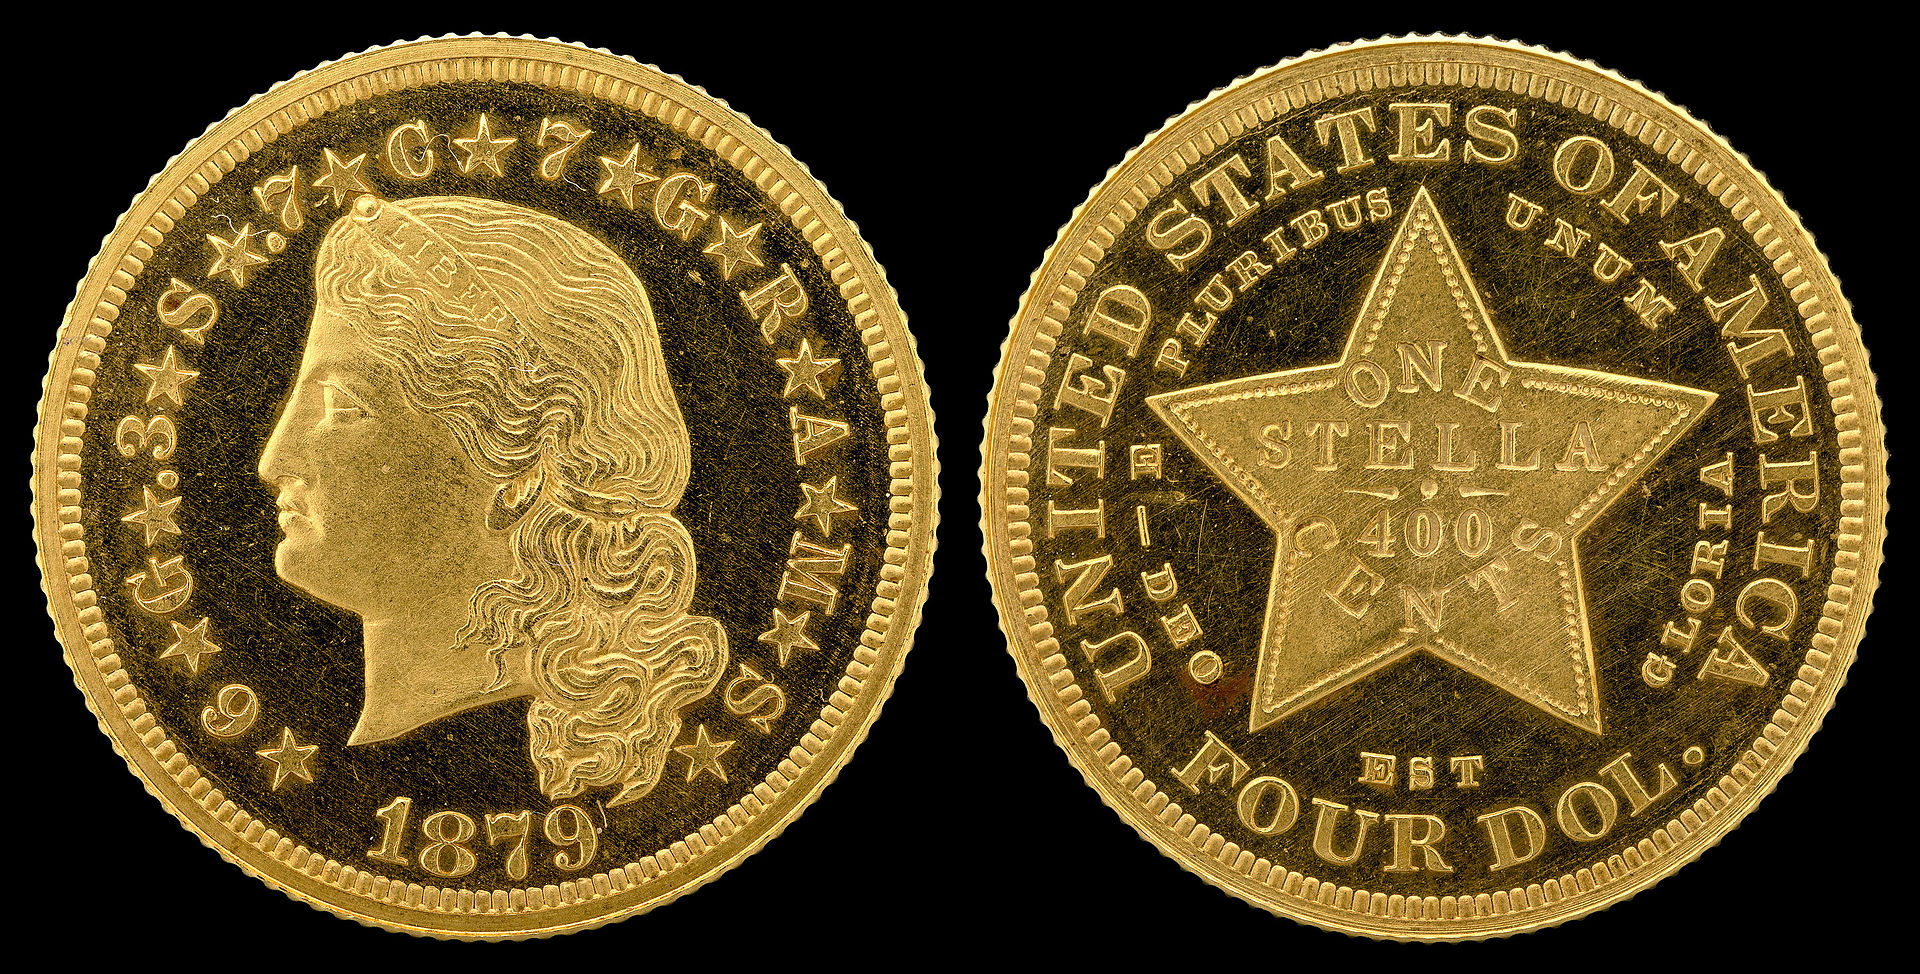
\includegraphics[width=1.0\textwidth]{4Dollar.jpg}
        \caption{4-Dollarmünze \enquote{Stella}}
        \label{subfig:4Dollar}
    \end{subfigure}
    \begin{subfigure}[b]{0.45\textwidth}
        \centering
        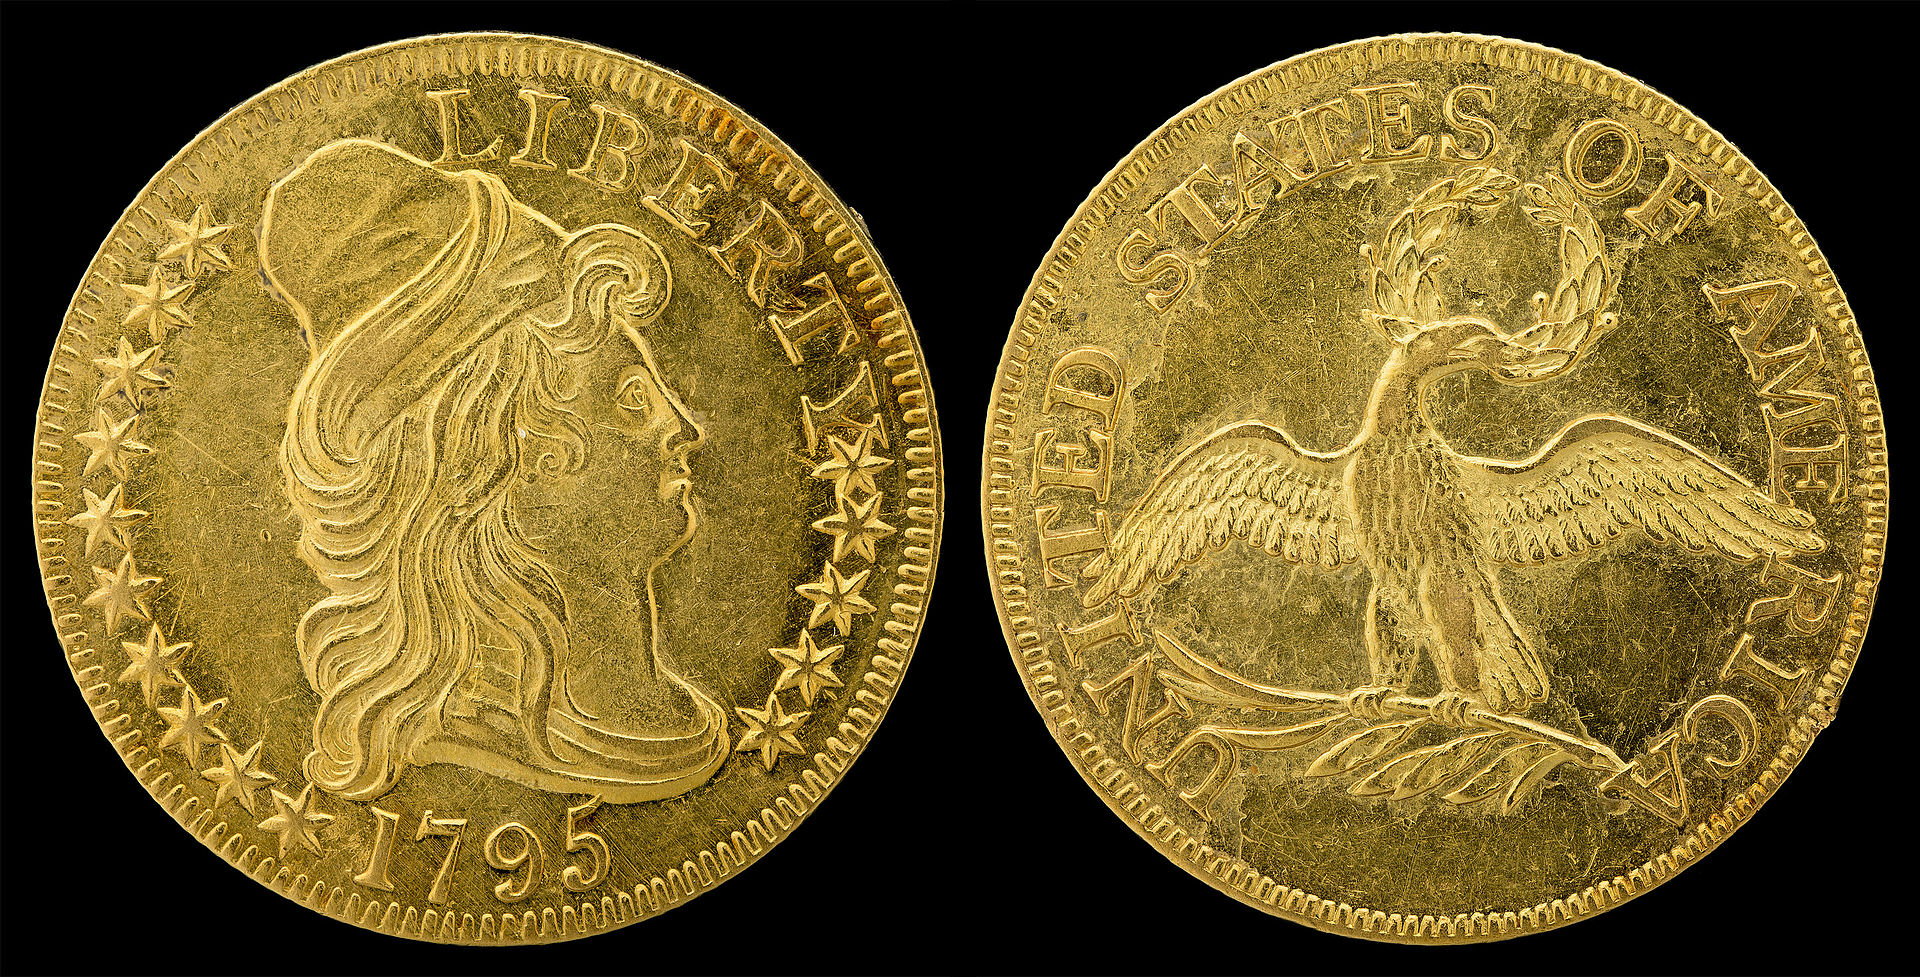
\includegraphics[width=1.0\textwidth]{5Dollar.jpg}
        \caption{5-Dollarmünze \enquote{half eagle}}
        \label{subfig:5Dollar}
    \end{subfigure}
    \caption{US-amerikanische 4-Dollarmünze und 5-Dollarmünze}
    \label{fig:Coins}
\end{figure}
\noindent
Doug findet es schade, dass diese Münzen nicht mehr geprägt werden. Schliesslich liesse sich jeder ganzzahlige Dollar-Betrag, der grösser als 11 Dollar ist, alleine durch eine Kombination dieser beiden Münzen auszahlen. Dies natürlich nur unter der Annahme, dass beliebig viele Exemplare von beiden Münzen zur Verfügung stehen.

Als kritische Menschen, sind wir nicht bereit, Doug einfach so zu glauben. Um Dougs Behauptung zu überprüfen, verwenden wir die starke Induktion (\cref{satz:starkeInduktion}). Wir definieren für jedes $n\in\N$ die Aussage $\mathcal{A}(n)$ als
\begin{center}
    $\mathcal{A}(n) :\iff $ \enquote{Der Dollar-Betrag $n$ kann durch eine Kombination aus 4-Dollarmünzen und 5-Dollarmünzen ausbezahlt werden.}
\end{center}
Dougs Behauptung besagt also, dass $\mathcal{A}(n)$ für jedes $n\in\N$ mit $n\geq 12$ gilt.

Der Betrag $n_0 = 12$ kann wegen $12 = 3\cdot 4 + 0\cdot 5$ durch drei 4er und null 5er ausbezahlt werden. Somit stimmt $\mathcal{A}(n_0)=\mathcal{A}(12)$. Zum Nachweis von $\mathcal{A}(n_0+1)=\mathcal{A}(13)$ dürften wir $\mathcal{A}(12)$ verwenden. Zum Nachweis von $\mathcal{A}(14)$ dürften wir $\mathcal{A}(12)$ und $\mathcal{A}(13)$ verwenden und zum Nachweis von $\mathcal{A}(15)$ gar $\mathcal{A}(12), \mathcal{A}(13)$ und $\mathcal{A}(14)$. Wir sehen jedoch sofort, dass
\begin{align*}
    13 &= 2\cdot 4 + 1\cdot 5, \quad 14 = 1\cdot 4 + 2\cdot 5, \quad 15 = 0\cdot 4 + 3\cdot 5
\end{align*}
und somit sind nebst $\mathcal{A}(12)$ auch $\mathcal{A}(13), \mathcal{A}(14)$ und $\mathcal{A}(15)$ nachgewiesen.

Sei nun $n\in\N$ mit $n\geq 15$. Wir beweisen, dass aus der Richtigkeit von $\mathcal{A}(k)$ für $12\leq k \leq n$ die Richtigkeit von $\mathcal{A}(n+1)$ folgt. Wir betrachten den Dollar-Betrag $n+1-4$. Offensichtlich gilt $12\leq n+1-4\leq n$. Gemäss (starker) Induktionsannahme kann der Betrag $n+1-4$ aber durch eine Kombination aus 4-Dollarmünzen und 5-Dollarmünzen ausbezahlt werden. Dies ist Aussage $\mathcal{A}(n+1-4) = \mathcal{A}(n-3)$. Durch das Hinzufügen einer einzigen 4-Dollarmünze zu dieser Kombination, erhalten wir eine gewünschte Auszahlung des Dollar-Betrags $n+1$.
}

\begin{aufgabe}{aufgabe:0208}
(*) Diese Aufgabe bezieht sich auch \cref{beispiel:Coins}. Schreiben Sie ein einfaches Python-Programm, welches für einen gegebenen ganzzahligen Dollar-Betrag $n\geq 12$ sämtliche möglichen Auszahlungen durch 4-Dollarmünzen und 5-Dollarmünzen ausgibt.

\noindent
Tipp: Verwenden Sie eine geschachtelte Schleife (eine Doppel-Schleife).
\end{aufgabe}
\begin{antwort}{aufgabe:0208}
\begin{lstlisting}[language=Python,caption=Dollar-Betrag auszahlen]
import math

def pay(n):
    combs = []
    amax = int(math.ceil(n / 4)) + 1
    bmax = int(math.ceil(n / 5)) + 1
    for a in range(amax):
        for b in range(bmax):
            if (4*a + 5*b) == n:
                combs.append((a,b))
    return combs
\end{lstlisting}
\end{antwort}

\noindent
Wir sind noch ein Beweis von \cref{satz:starkeInduktion} schuldig:

\beweis{
Wir beweisen \cref{satz:starkeInduktion}. Angenommen der Satz sei falsch und somit $\mathcal{A}(n)$ nicht jedes $n\geq n_0$ richtig. Dann ist die Menge
\begin{align*}
    N := \setct{n\in\N}{$n\geq n_0$ und $\mathcal{A}(n)$ ist falsch}
\end{align*}
nichtleer. Gemäss \cref{satz:MinimumN} besitzt die Menge $N$ ein minimales Element $m$. Da $\mathcal{A}(n_0)$ wegen Bedingung (i) richtig ist, muss $m>n_0$ gelten. Es existiert eine eindeutige natürliche Zahl $n$ mit $n+1 = m$. Aufgrund der Definition von $m$ gilt, dass die Aussagen $\mathcal{A}(k)$ für alle natürlichen Zahlen $k$ mit $n_0\leq k\leq n$ richtig sind. Dann garantiert Bedingung (ii) aber die Richtigkeit von $\mathcal{A}(n+1) = \mathcal{A}(m)$. Doch dies ist nach der Definition von $m$ unmöglich und wir haben einen Widerspruch gefunden.
}

\begin{aufgabe}{aufgabe:0210}
Der junge Tim besitzt beliebig viele Holzklötze der Länge 7 und beliebig viele der Länge 8. Klötze anderer Längen hat er keine.
\begin{aenum}
    \item Tim weiss, dass sein Plüschkrokodil die Länge 38 hat. Nun möchte er mit seinen Klötzen eine Strecke derselben Länge bauen. Doch bislang blieben alle seine Versuche erfolglos. Helfen Sie Tim, indem Sie ein Python-Programm schreiben, welches Ihnen angibt, wie viele Klötze der Länge 7 und wie viele der Länge 8 benötigt werden, um die Strecke zu bauen.
    \item Weisen Sie nach, dass es mit Tims Klötzen nicht möglich ist, eine Strecke der Länge 41 zu bauen. Schreiben Sie dazu ein Python-Programm, welches alle denkbaren Möglichkeiten ausprobiert.
    \item Beweisen Sie mit Hilfe von \cref{satz:starkeInduktion} zur starken Induktion, dass jede Strecke der Länge $n\in\N$ mit $n\geq 42$ mit Tims Klötzen gebaut werden kann.
\end{aenum}
\end{aufgabe}
\begin{antwort}{aufgabe:0210}
\begin{aenum}
    \item Das entsprechende Programm ist in \cref{listing:tim} gegeben.
\begin{lstlisting}[language=Python,caption=Bauklötze,label=listing:tim]
import math

def klotz(n):
    combs = []
    amax = int(math.ceil(n / 7)) + 1
    bmax = int(math.ceil(n / 8)) + 1
    for a in range(amax):
        for b in range(bmax):
            if (7*a + 8*b) == n:
                combs.append((a,b))
    return combs

print(klotz(38))
print(klotz(41))
\end{lstlisting}
    \item siehe (a)
    \item
Wir definieren für jedes $n\in\N$ die Aussage $\mathcal{A}(n)$ als
\begin{center}
    $\mathcal{A}(n) :\iff $ \enquote{Die Strecke der Länge $n$ kann durch eine Kombination aus Klötzen der Längen 7 und 8 gebaut werden.}
\end{center}
Die Strecke $n_0 = 42$ kann wegen $42 = 6\cdot 7 + 0\cdot 8$ gebaut werden. Somit stimmt $\mathcal{A}(n_0)=\mathcal{A}(42)$. Zum Nachweis von $\mathcal{A}(n_0+1)=\mathcal{A}(43)$ dürften wir $\mathcal{A}(42)$ verwenden. Zum Nachweis von $\mathcal{A}(44)$ dürften wir $\mathcal{A}(42)$ und $\mathcal{A}(43)$ verwenden und zum Nachweis von $\mathcal{A}(45)$ gar $\mathcal{A}(42), \mathcal{A}(43)$ und $\mathcal{A}(44)$, und so weiter. Wir sehen jedoch sofort, dass
\begin{align*}
    43 &= 5\cdot 7 + 1\cdot 8, \quad 44 = 4\cdot 7 + 2\cdot 8, \quad 45 = 3\cdot 7 + 3\cdot 8 \\
    46 &= 2\cdot 7 + 4\cdot 8, \quad 47 = 1\cdot 7 + 5\cdot 8, \quad 48 = 0\cdot 7 + 6\cdot 8
\end{align*}
und somit sind nebst $\mathcal{A}(42)$ auch $\mathcal{A}(s)$ für $s\in\lrc{43,44,45,46,47,48}$ nachgewiesen.

Sei nun $n\in\N$ mit $n\geq 48$. Wir beweisen, dass aus der Richtigkeit von $\mathcal{A}(k)$ für $42\leq k \leq n$ die Richtigkeit von $\mathcal{A}(n+1)$ folgt. Wir betrachten die Strecke der Länge $n+1-7$. Offensichtlich gilt $42\leq n+1-7\leq n$. Gemäss (starker) Induktionsannahme kann die Strecke der Länge $n+1-7$ aber durch eine Kombination aus Klötzen der Längen 7 und 8 gebaut werden. Dies ist Aussage $\mathcal{A}(n+1-7) = \mathcal{A}(n-6)$. Durch das Ansetzen eines Klotzes der Länge 7 zu dieser Kombination, erhalten wir eine Strecke der Länge $n+1$.
\end{aenum}
\end{antwort}

\begin{aufgabe}{aufgabe:0310}
Seien $+$ und $\cdot$ assoziative und kommutative Verknüpfungen auf einer Menge $X$, welche das Distributivgesetz:
\begin{align*}
    (x+y)\cdot z = x\cdot z + y\cdot z
\end{align*}
für $x,y,z\in X$ erfüllen. Beweisen Sie mit Hilfe von \cref{satz:starkeInduktion} zur starken Induktion die Richtigkeit des \enquote{verallgemeinerten} Distributivgesetztes:
\begin{align*}
    \mathcal{A}(n) :\iff c\sum_{k=0}^n\lr{x_k} = \sum_{k=0}^n\lr{cx_k}
\end{align*}
für alle $n\in\N$. Dabei sind $c\in X$ und $(x_k)$ eine Folge in $X$. 
\end{aufgabe}
\begin{antwort}{aufgabe:0310}
Aussage $\mathcal{A}(0)$ ist offensichtlich richtig.

Wir zeigen nun, dass aus der Richtigkeit von $\mathcal{A}(k)$ für $0\leq k\leq n$ die Richtigkeit von $\mathcal{A}(n+1)$ folgt. Dazu betrachten wir:
\begin{align*}
    &c\sum_{k=0}^{n+1}\lr{x_k} = \\
    &c\lr{x_{n+1} + \sum_{k=0}^{n}\lr{x_k}} \stackrel{\text{Distributivgesetz}}{=} \\
    &cx_{n+1} + c\sum_{k=0}^{n}\lr{x_k} \stackrel{\text{Induktionsvoraussetzung}}{=} \\
    &cx_{n+1} + \sum_{k=0}^{n}\lr{cx_k} = \\
    &\sum_{k=0}^{n+1}\lr{cx_k}.
\end{align*}
Mit dem Prinzip der starken Induktion folgt somit, die Richtigkeit der Aussage $\mathcal{A}(n)$ für alle $n\in\N$.
\end{antwort}

% 4-Dollar Stella
% US Mint (coin), National Numismatic Collection (photograph by Jaclyn Nash) - National Numismatic Collection, National Museum of American History
% 5-Dollar half eagle
% US Mint (coin), National Numismatic Collection (photograph by Jaclyn Nash) - National Numismatic Collection, National Museum of American History
\clearpage
\shipoutAnswer % Das Induktionsprinzip
        \chapter{Rekursion}\label{ch:Kapitel03}

\section{Fakultät}\label{sec:fakultaet}
Drei (unterscheidbare) Personen $A, B$ und $C$ stellen sich in der Mensa in einer Warteschlange an. Wie viele verschiedene Warteschlangen sind möglich? In der vordersten Position der Warteschlange platzieren wir eine der drei Personen $A, B$ oder $C$. Für die vorderste Position haben wir also drei Wahlmöglichkeiten. In der mittleren Position muss genau eine der verbleibenden zwei Personen positioniert werden (zwei Wahlmöglichkeiten). Die hinterste Position muss schliesslich von der noch verbleibenden Person besetzt werden (eine Möglichkeit). Insgesamt gibt es also (gemäss den Rechengesetzen der Kombinatorik)
\begin{align*}
    3\cdot 2\cdot 1 = 6
\end{align*}
verschiedene Möglichkeiten, drei Personen in einer Reihe anzuordnen. Analog sieht man ein, dass es
\begin{align*}
    n\cdot (n-1)\cdot\ldots\cdot 3\cdot 2\cdot 1
\end{align*}
Möglichkeiten gibt, $n\in\N$ Personen in einer Warteschlange anzuordnen. Es gibt eine Möglichkeit, $0$ Personen anzuordnen, nämlich in der \enquote{leeren Warteschlange}.
\beispiel{-}
{Es gibt $5\cdot 4\cdot 3\cdot 2\cdot 1 = 120$ Möglichkeiten, fünf Personen in einer Reihe anzuordnen.}

\noindent
Da das Produkt $n\cdot (n-1)\cdot\ldots\cdot 3\cdot 2\cdot 1$ häufig in Erscheinung tritt, besitzt es einen eigenen Namen: Die \textit{Fakultät} von $n$ und wird $n!$ geschrieben. So ist zum Beispiel $5! = 5\cdot 4\cdot 3\cdot 2\cdot 1 = 120$.

\begin{aufgabe}{aufgabe:0301}
Wir gehen davon aus, dass Sie bereits das Produkt $12!$  berechnet haben. Wie können Sie dieses Vorwissen einsetzen, um $13!$ relativ schnell zu berechnen? Wie lässt sich für $n\in\Nunit$ die Fakultät $n!$ aus $(n-1)!$ berechnen?
\end{aufgabe}
\begin{antwort}{aufgabe:0301}
Wir beobachten, dass $13! = 13\cdot 12!$ gilt. Somit müssen wir $12!$ lediglich mit $13$ multiplizieren um $13!$ zu erhalten. Für $n\in\Nunit$ gilt allgemein
\begin{align*}
    n! = n\cdot (n-1)!.
\end{align*}
\end{antwort}

\noindent
Die in \cref{aufgabe:0301} gemachte Beobachtung ist zwar einfach, hat aber dennoch bedeutende Implikationen. Um $5!$ zu berechnen, müssen wir lediglich multiplizieren können und wissen, wie $4!$ berechnet wird. Das Problem der Berechnung von $5!$ lässt sich also auf eine Multiplikation und die Berechnung von $4!$ reduzieren. Doch genau gleich verhält es sich mit dem Problem der Berechnung von $4!$. Diese Reduktion auf immer kleinere aber gleichartige Probleme kann solange fortgeführt werden, bis wir bei $0!$ ankommen. Betrachten Sie die folgende Berechnung:
\begin{align*}
    \textcolor{Red}{5!} &= 5\cdot\underbrace{4\cdot 3\cdot 2\cdot 1}_{\textcolor{Blue}{4!}} \\
    \textcolor{Blue}{4!} &= 4\cdot\underbrace{3\cdot 2\cdot 1}_{\textcolor{Green}{3!}} \\
    \textcolor{Green}{3!} &= 3\cdot\underbrace{2\cdot 1}_{\textcolor{Goldenrod}{2!}} \\
    \textcolor{Goldenrod}{2!} &= 2\cdot\underbrace{1}_{\textcolor{Fuchsia}{1!}} \\
    \textcolor{Orchid}{1!} &= 1\cdot\underbrace{0!}_{1} = 1
\end{align*}
Durch \enquote{Rückwertseinsetzen} erhalten wir nun den Wert für $5!$:
\begin{align*}
    \textcolor{Orchid}{1!} &= 1\cdot 0! = 1 \\
    \textcolor{Goldenrod}{2!} &= 2\cdot\textcolor{Orchid}{1!} = 2\cdot 1 = 2 \\
    \textcolor{Green}{3!} &= 3\cdot \textcolor{Goldenrod}{2!} = 3\cdot 2 = 6 \\
    \textcolor{Blue}{4!} &= 4\cdot\textcolor{Green}{3!} = 4\cdot 6 = 24 \\
    \textcolor{Red}{5!} &= 5\cdot\textcolor{Blue}{4!} = 5\cdot 24 = 120.
\end{align*}

\noindent
Nach diesen Betrachtungen ist plausibel, dass Folgendes eine sinnvolle Definition der \tib{Fakultät}\index{Fakultät} ist:
\begin{definition}[Fakultät]{definition:fac}
Es sei $n$ eine natürliche Zahl. Dann definieren wir die Fakultät $n!$ von $n$ durch
\begin{align}\label{eq:fakultaet}
n! := 
  \begin{cases}
    1, &\text{falls $n=0$, (Rekursionsanfang)} \\
    n(n-1)!, & \text{falls  $n\geq 1$. (Rekursionsschritt)}
  \end{cases}
\end{align}
\end{definition}

\noindent
Beachten Sie, dass \cref{definition:fac} der Fakultät selbst die Fakultät verwendet! Eine auf diese Weise definierte Funktion wird \tib{rekursiv}\index{rekursiv} genannt.

\section{Finde den Star! (konstruktive Induktion)}
Das folgende Beispiel stammt aus \cite{Datenstrukturen}. In einem Raum befinden sich $n\in\N$ Personen, wobei $n\geq 2$ ist. Wir wollen den \textit{Star} unter diesen $n$ Personen finden. Ein Star ist definiert als eine Person, welche niemanden anderen kennt, jedoch von allen gekannt wird. Die einzige erlaubte \textit{Operation} um einen Star zu identifizieren, ist eine Person $A$ zu fragen:
\begin{center}
    \enquote{\textcolor{Red}{Kennst Du Person $B$?}},
\end{center}
wobei $A\neq B$ gilt.

\begin{aufgabe}{aufgabe:0350}
    Begründen Sie, warum es unter $n$ Personen in einem Raum nicht zwei verschiedene Stars geben kann.
\end{aufgabe}
\begin{antwort}{aufgabe:0350}
Angenommen es gäbe zwei Stars $S_1$ und $S_2$ in dem Raum. Da $S_2$ ein Star ist, wird $S_2$ von allen anderen gekannt. Insbesondere kennt $S_1$ die Person $S_2$. Damit kann aber $S_1$ selbst kein Star sein. Dies ist ein Widerspruch zu unserer Annahme, dass sowohl $S_1$ als auch $S_2$ Stars sind.
\end{antwort}
\noindent
Wir wollen einen Star in Raum mit möglichst wenig Fragen (Operationen) finden. Eine naive Lösung besteht darin, jede Person über jede andere zu befragen. Für $n=4$ könnte ein Resultat einer solchen Befragung wie folgt aussehen:
\begin{table}[H]
\centering
    \begin{tabular}{ccccc}
    -                                        & 1    & 2  & 3    & $\textcolor{Blue}{4}$   \\
    1                                       & -    & Ja & Nein & Nein                                     \\
    $\textcolor{Green}{2}$ & Nein & -  & Nein & $\textcolor{Red}{Nein}$ \\
    3                                       & Ja   & Ja & -    & Nein                                     \\
    4                                       & Ja   & Ja & Ja   & -                                       
    \end{tabular}
\end{table}
\noindent
Dabei bedeutet der Eintrag $\textcolor{Red}{Nein}$, dass Person $\textcolor{Green}{2}$ die Person $\textcolor{Blue}{4}$ nicht kennt und somit die Frage \enquote{Kennst Du Person 4?} mit \enquote{Nein} beantwortet. Hier ist Person 2 der Star. Bei $n$ Personen sind bei diesem Vorgehen offensichtlich $n(n-1)$ Fragen gestellt (jede der $n$ Personen wird zu allen $n-1$ anderen befragt).

Wir wollen versuchen, die Anzahl der Fragen zu reduzieren. Dazu wenden wir ein Vorgehen an, welches manchmal \textit{konstruktive Induktion} genannt wird. Wir zerlegen das Problem, den Star unter $n$ Personen zu finden, in kleinere Probleme:
\begin{itemize}
    \item Für $n=2$ genügen zwei Fragen.
    \item Sei $n>2$: Schicke eine Person $A$ weg. Finde nun den Star unter $n-1$ Personen (kleineres Problem). Überprüfe danach $A$ mit $2(n-1)$ Fragen.
\end{itemize}
Doch dieses Vorgehen können wir weiter fortsetzen und dieselbe Strategie auf das Problem mit $n-1$ Personen (das kleinere Problem) anwenden. Schliesslich gelangen wir bei dem Problem mit 2 Personen an, für welches zwei Fragen genügen. Insgesamt stellen wir also
\begin{align*}
    F(n) &= \\
    &2(n-1) + F(n-1) =\\
    &2(n-1) + 2(n-2) + F(n-2) =\\
    &2(n-1) + 2(n-2) + 2(n-3) + F(n-3) =\\
    &\quad\quad\quad\quad\quad\quad\quad\quad\quad\vdots \\
    &2(n-1) + 2(n-2) + 2(n-3) + 2(n-4) + \ldots + 2 =\\
    &2(1 + 2 + 3 +\ldots + (n-2) + (n-1)) \stackrel{\text{kleiner Gauss}}{=} \\
    &2\lr{\frac{n(n-1)}{2}} = \\
    &n(n-1).
\end{align*}
Somit haben wir gegenüber der ursprünglichen naiven Lösung (befrage alle zu allen) nichts gewonnen. Zum Glück ist es aber kein grosser Aufwand unseren Ansatz der konstruktiven Induktion stark zu verbessern und somit zu retten. Die Idee der Verbesserung besteht darin, sicherzustellen, dass die Person, welche wir aus dem Raum schicken, kein Star ist.
\begin{aufgabe}{aufgabe:0351}
Erklären Sie, warum eine einzige Frage an eine beliebige Person im Raum stets genügt, um eine Person zu identifizieren, welche sicherlich kein Star ist.
\end{aufgabe}
\begin{antwort}{aufgabe:0351}
\begin{itemize}
    \item Frage eine beliebige Person $A$ im Raum, ob sie eine andere beliebige Person $B$ kennt.
    \item Falls $A$ die Person $B$ kennt $\Rightarrow A$ ist kein Star.
    \item Falls $A$ die Person $B$ nicht kennt $\Rightarrow B$ ist kein Star.
\end{itemize}
In jedem der Fälle haben wir mit einer einzigen Frage eine Person identifiziert, welche sicherlich kein Star ist.
\end{antwort}
\noindent
Zum Schluss bleiben zwei Personen, von denen möglicherweise eine Person $X$ der Star ist. Wir überprüfen mit jeder Person, die draussen ist, ob $X$ ein Star sein kann. Mit dieser Verbesserung erhalten wir $F(2) = 2$ und $F(n) = 1 + F(n-1) + 2$ für $n\geq 3$, also insgesamt:
\begin{align}\label{eq:star}
    F(n) =
    \begin{cases}
        2, &\text{falls $n=2$,} \\
        F(n) = 1 + F(n-1) + 2, & \text{falls  $n\geq 3$.}
      \end{cases}
\end{align}
Ähnlich wie bei unserer Betrachtung der Fakultät, sehen wir auch hier, dass sich die Bestimmung der Anzahl benötigter Fragen $F(n)$ bei $n$ Personen auf die Bestimmung des kleineren (aber analogen) Problems $F(n-1)$ reduzieren lässt.
\begin{aufgabe}{aufgabe:0352}
Wir haben für die benötigten Fragen $F(n)$ für einen Raum mit $n$ Personen die Beziehung in \cref{eq:star} gefunden. Wir vermuten, dass wir den Wert für $F(n)$ durch wiederholte Reduktion auf kleinere Probleme wie folgt \enquote{entpacken} können:
\begin{align*}
    F(n) = 3 + F(n-1) = 2\cdot 3 + F(n-2) = \ldots = 3\cdot (n-2) + 2 = 3n - 4.
\end{align*}
Beweisen Sie durch vollständige Induktion, dass $F(n) := 3n - 4$ tatsächlich \cref{eq:star} erfüllt. Berechnen Sie schliesslich, wie viele Fragen wir mit diesem Verfahren bei $n = 1000$ Personen benötigen.
\end{aufgabe}
\begin{antwort}{aufgabe:0352}
Der Induktionsanfang ist klar, denn für $n = 2$ benötigen wir genau zwei Fragen. Sei nun die Behauptung für ein $n\in\N$ mit $n\geq 2$ wahr. Dann gilt
\begin{align*}
    F(n+1) = F(n) + 3 = 3n-4 + 3 = 3n - 1,
\end{align*}
doch dies ist genau die Behauptung, denn $3(n+1)-4 = 3n+3-4=3n-1$.

Gemäss der soeben bewiesenen Formel, sind mit unserem Vorgehen genau $F(1000) = 3\cdot 1000 - 4 = 2996$ Fragen notwendig. Beachten Sie, dass wir in keinster Weise behaupten, dass dieses Vorgehen optimal ist.
\end{antwort}

\clearpage
\section{Rekursion in Algorithmen}
In diesem Abschnitt wollen wir beginnen zu verstehen, wie Probleme rekursiv mit Hilfe von Programmen gelöst werden können. Zum Einstieg betrachten wir nochmals die (rekursive) Definition der Fakultät in \cref{eq:fakultaet}. Lassen Sie uns an dieser Stelle wagemutig sein! Wir \enquote{übersetzen} die Definition direkt in die Python-Programmiersprache und lassen uns von dem Ergebnis überraschen:
\begin{lstlisting}[language=Python,caption=rekursive Fakultäts-Funktion]
def factorial(n):
    if n == 0:
        return 1 # Rekursionsanfang
    else:
        return n * factorial(n-1) # Rekursionsschritt
\end{lstlisting}
Wir haben \cref{definition:fac} praktisch eins zu eins \enquote{abgetippt}. Beachten Sie, dass in der Definition der Funktion \pythoninline{factorial} die Funktion \pythoninline{factorial} selbst verwendet wird. Wie und warum funktioniert dieses Vorgehen? \cref{listing:lowtech} zeigt schematisch auf, wie der Funktionsaufruf \pythoninline{factorial(3)} abgearbeitet wird. Beachten Sie die Ähnlichkeit zu unserer Diskussion in \cref{sec:fakultaet}. 

\lstset{basicstyle=\ttfamily\footnotesize}
\begin{lstlisting}[language=Python,caption=rekursive Berechnung der Fakultät,label=listing:lowtech]
## anfängliche Aufrufe ##

# Aufruf 0:
factorial(3)
return 3 * factorial(2) # Rekursionsschritt (Zeile 5)
                |
                |
                v 
           # Aufruf 1:
           factorial(2)
           return 2 * factorial(1) # Rekursionsschritt (Zeile 5)
                           |
                           |
                           v
                      # Aufruf 2:
                      factorial(1)
                      return 1 * factorial(0) # Rekursionsschritt (Zeile 5)
                                      |
                                      |
                                      v
                                 # Aufruf 3:
                                 factorial(0)
                                 return 1 # Rekursionsanfang (Zeile 2)

## Rückwertseinsetzen ##
factorial(1) = 1 * factorial(0) = 1 * 1 = 1
factorial(2) = 2 * factorial(1) = 2 * 1 = 2
factorial(3) = 3 * factorial(2) = 3 * 2 = 6
\end{lstlisting}
\lstset{style=mystyle}
\noindent
Der anfängliche Aufruf \pythoninline{factorial(3)} löst (rekursiv) in seinem \pythoninline{return} auf (seiner) Zeile 5 den Aufruf \pythoninline{factorial(2)} aus. Dieser löst rekursiv einen weiteren Funktionsaufruf aus. Dies geht so lange weiter, bis zum ersten Mal ein Aufruf den Rekursionsanfang (Zeile 2) erreicht. Danach können die noch ausstehenden \pythoninline{return}-Statements endlich komplettiert werden (Rückwertseinsetzen).

\clearpage

\begin{aufgabe}{aufgabe:0303}
Sei $a\in\R$ und $n$ eine natürliche Zahl. Wir definieren den Potenzausdruck $a^n$ rekursiv durch
\[
  a^n := 
  \begin{cases}
    1, &\text{falls $n=0$, (Rekursionsanfang)} \\
    a\cdot a^{n-1}, & \text{falls  $n\geq 1$. (Rekursionsschritt)}
  \end{cases}
\]
Implementieren Sie eine Python-Funktion \pythoninline{def potenz(a,n)}, welche $a^n$ gemäss dieser rekursiven Definition berechnet.
\end{aufgabe}
\begin{antwort}{aufgabe:0303}
\begin{lstlisting}[language=Python,caption=rekursive Potenz-Funktion]
def potenz(a,n):
    if n == 0:
        return 1
    else:
        return a * potenz(a,n-1)
\end{lstlisting}
\end{antwort}

\begin{aufgabe}{aufgabe:0302}
Implementieren Sie eine Python-Funktion \pythoninline{def factorial_loop(n)}, welche
\begin{align*}
    n! = n\cdot (n-1)\cdot\ldots\cdot 3\cdot 2\cdot 1
\end{align*}
nicht rekursiv, sondern mit Hilfe einer einzigen Schleife (\pythoninline{for}-loop) berechnet.
\end{aufgabe}
\begin{antwort}{aufgabe:0302}
\begin{lstlisting}[language=Python,caption=rekursive Potenz-Funktion]
def factorial_loop(n):
    factorial = 1
    if n == 0:
        return factorial
    else:
        for k in range(1,n+1):
            factorial *= k
        return factorial
\end{lstlisting}
\end{antwort}

\begin{aufgabe}[The One]{aufgabe:0304}
Sie arbeiten für eine respektable Softwareentwicklungsfirma. Ihr Arbeitskollege \textit{Thomas A. Anderson} hat folgende Python-Funktion zu Ihrem Softwareprojekt hinzugefügt:
\begin{lstlisting}[language=Python]
# m und n sind natürliche Zahlen
def unbekannt(m,n):
    if m == 0:
        return 0
    else:
        return unbekannt(m-1,n) + n
\end{lstlisting}
\begin{aenum}
    \item Handelt es sich bei \pythoninline{unbekannt} um eine rekursiv oder nicht rekursiv definierte Funktion? Begründen Sie Ihre Antwort.
    \item Thomas A. Anderson hat sich schon einige Tage nicht in der Firma blicken lassen und Sie können ihn telefonisch nicht erreichen. Abgesehen von dem Kommentar in Zeile 1, hat er die Funktion \pythoninline{unbekannt} nicht dokumentiert und der Name der Funktion hilft uns nicht weiter. Erklären Sie genau, was die Funktion tut und geben Sie ihr einen treffenden Namen.
    
    \noindent
    Tipp: Berechnen Sie die Werte
    \begin{itemize}
        \item \pythoninline{unbekannt(0,4)},
        \item \pythoninline{unbekannt(1,4)},
        \item \pythoninline{unbekannt(2,4)},
        \item und \pythoninline{unbekannt(3,4)}
    \end{itemize}
    \enquote{von Hand} und leiten Sie daraus ab, was die Funktion tut.
    \item Was ist der Rückgabewert von \pythoninline{unbekannt(100,50)}?
\end{aenum}
\end{aufgabe}
\begin{antwort}{aufgabe:0304}
\begin{aenum}
    \item Die Python-Funktion ist rekursiv definiert, da sie sich selbst aufruft.
    \item Die unbekannte Funktion multipliziert die Zahlen $m$ und $n$, realisiert also die Operation $m\cdot n$. In der Tat sieht man, dass die Funktion so lange $n$ addiert, bis $m = 0$ ist. Ein treffender Name für die Funktion wäre zum Beispiel \pythoninline{mult(m,n)}.
    \item Der Rückgabewert ist $100\cdot 50 = 5000$.
\end{aenum}
\end{antwort}

\clearpage
\begin{aufgabe}{aufgabe:0305}
In Python ist eine Liste \pythoninline{L} von reellen Zahlen gegeben. Schreiben Sie eine Python-Funktion \pythoninline{sum_rek(L)}, welche rekursiv die Summe der Zahlen in der Liste berechnet. Es kann angenommen werden, dass die Länge der Liste $\geq 1$ ist.
\begin{lstlisting}[language=Python]
Beispiel 1:
Eingabe: L = [1,3,2,10]
Ausgabe: 16

Beispiel 2:
Eingabe: L = [1,-1,2,5,4]
Ausgabe: 11

\end{lstlisting}
\end{aufgabe}
\begin{antwort}{aufgabe:0305}
\begin{lstlisting}[language=Python]
def sum_rek(L):
    if len(L) == 1:
        return L[0]
    else:
        return sum_rek(L[:-1]) + L[-1]
\end{lstlisting}
\end{antwort}


\begin{aufgabe}{aufgabe:0377}
Ein Wort heisst \textit{Palindrom}, falls das Wort vorwärts und rückwärts genau gleich gelesen wird.\\
Beispiele:
\begin{itemize}
    \item neben
    \item Rentner
    \item Otto
    \item Lagerregal.
\end{itemize}
Das \textit{leere Wort}, also das Wort der Länge $0$, ist ebenfalls ein Palindrom. Schreiben Sie ein rekursives Python-Programm, welches entscheidet, ob ein gegebenes Wort \verb|w| ein Palindrom ist oder nicht.
\end{aufgabe}

\begin{antwort}{aufgabe:0377}
\begin{lstlisting}[language=Python]
def check_palindrom(w):
    w = w.upper()
    if len(wort) <= 1:
        return True
    elif w[0] != w[-1]:
        return False
    return check_palindrom(w[1:-1])
\end{lstlisting}
oder noch kürzer:
\begin{lstlisting}[language=Python]
def check_palindrom(w):
    return (True if len(w) <= 1 else (check_palindrom(w[1:-1]) if w[0].lower() == w[-1].lower() else False))
\end{lstlisting}
\end{antwort}

\begin{aufgabe}{aufgabe:0308}
Schreiben Sie eine Python-Funktion \pythoninline{summe(n)}, welche die Summe
\begin{align*}
    \sum_{k=0}^n k := 0 + 1 + \ldots + n.
\end{align*}
der ersten $n+1$ natürlichen Zahlen $0,1,\ldots ,n$ rekursiv berechnet.
\end{aufgabe}
\begin{antwort}{aufgabe:0308}
\begin{lstlisting}[language=Python,caption=rekursive Berechnung einer Summe]
def summe(n):
    if n == 0:
        return 0
    else:
        return n + summe(n-1)
\end{lstlisting}
\end{antwort}

\begin{aufgabe}{aufgabe:0311}
Schreiben Sie eine Python-Funktion \pythoninline{produkt(n)}, welche das Produkt
\begin{align*}
    \prod_{k=1}^n k^3 := 1 \cdot 8 \cdot \ldots \cdot n^3
\end{align*}
für $n\in\Nunit$ rekursiv berechnet.
\end{aufgabe}
\begin{antwort}{aufgabe:0311}
\begin{lstlisting}[language=Python,caption=rekursive Berechnung eines Produkts]
def produkt(n):
    if n == 1:
        return 1
    else:
        return n**3 * produkt(n-1)
\end{lstlisting}
\end{antwort}

\clearpage

\section{Fibonacci-Folge}
In der zweiten Fassung des Buches \textit{Liber abbaci} (\enquote{Buch der Rechenkunst}) beschrieb der italienische Mathematiker \textit{Leonardo da Pisa}, bekannt als \textit{Fibonacci}, das Wachstum einer Kaninchenpopulation.

\begin{itemize}
    \item Jedes geschlechtsreife Paar Kaninchen wirft pro Monat genau ein neues Paar Kaninchen (ein Weibchen und ein Männchen). Die Austragungszeit (Dauer der Schwangerschaft) dauert bei Kaninchen also immer genau einen Monat. Jeden Monat kommt also eine neue Generation von Kaninchen zur Welt.
    \item Ein neugeborenes Paar von Kaninchen wird erst am Ende seines ersten Lebensmonats geschlechtsreif und wirft entsprechend erst Ende seines zweiten Lebensmonats sein erstes Paar Kaninchen.
    \item Kein Kaninchen stirbt, kein Kanninchen verlässt das betrachtete System und kein Kanninchen wird, ausser durch Geburt, in das System hineingebracht.
\end{itemize}
Sei $G_n$ die Anzahl der geschlechtsreifen Kaninchenpaare und $g_n$ die Anzahl der nicht geschlechtsreifen Kaninchenpaare der Generation $n$ für $n\in\N$. Beachten Sie, dass die gesamte Anzahl der Kaninchenpaare der Generation $n$ damit der Summe $F_n := G_n+g_n$ entspricht. Betrachten wir nun die obigen Regeln für das Wachstum einer Kaninchenpopulation für alle $n\in\N$. Es gilt
\begin{align}
    G_{n+2} = G_{n+1} + g_{n+1},
\end{align}
da die geschlechtsreifen Kaninchen $G_{n+1}$ der Generation $n+1$ auch einen Monat später noch geschlechtsreif sein werden und die nicht geschlechtsreifen Kaninchen $g_{n+1}$ der Generation $n+1$ einen Monat später geschlechtsreif sein werden. Völlig analog begründet man die Gleichung
\begin{align}
    G_{n+1} = G_{n} + g_{n}.
\end{align}
Des Weiteren gilt offensichtlich
\begin{align}
    g_{n+2}  = G_{n+1}.
\end{align}
Wir haben also drei Gleichungen für die Population:
\begin{align}\label{eq:Fib1}
    \textcolor{Blue}{G_{n+2}} = \textcolor{Red}{G_{n+1}} +  \textcolor{Blue}{g_{n+1}}
\end{align}
\begin{align}\label{eq:Fib2}
    \textcolor{Red}{G_{n+1}} = \textcolor{Red}{G_{n}} + \textcolor{Red}{g_{n}}
\end{align}
\begin{align}\label{eq:Fib3}
    \textcolor{Purple}{g_{n+2}}  = \textcolor{Purple}{G_{n+1}}
\end{align}

\noindent
Einsetzen von Gleichung \ref{eq:Fib2} in Gleichung \ref{eq:Fib1} liefert:
\begin{align*}
    \textcolor{Blue}{G_{n+2}} &= \textcolor{Red}{G_{n}} + \textcolor{Red}{g_{n}} + \textcolor{Blue}{g_{n+1}} \\
    &\iff \\
    \underbrace{\textcolor{Blue}{G_{n+2}} + \textcolor{Purple}{g_{n+2}}}_{F_{n+2}} &= \underbrace{\textcolor{Purple}{G_{n+1}} + \textcolor{Blue}{g_{n+1}}}_{F_{n+1}} + \underbrace{\textcolor{Red}{G_{n}} + \textcolor{Red}{g_{n}}}_{F_n}.
\end{align*}

\noindent
Für die Gesamtzahl der Population der Kaninchenpaare gilt also
\begin{align*}
    F_{n+2} = F_{n+1} + F_{n}
\end{align*}
für alle $n\in\N$. Für Generation $n=0$ definieren wir $G_0:=0$ und $g_0:=0$. Zu Beginn, also in der Generation $n=1$, wird ein erstes Paar von Kaninchen in das System eingeführt. Dieses erste Paar wird erst nach einem Monat geschlechtsreif. Es gilt also $G_1=0$ und $g_1=1$. Somit besteht die Generation $n=2$ immer noch aus nur einem Paar Kaninchen: $G_2=1$ und $g_2=0$. Die Generation $n=3$ aus zwei Paaren: $G_3=1$ und $g_3=1$. Logisch fortgeführt findet man die sogenannte \tib{Fibonacci-Folge}\index{Folge!Fibonacci-}:
\begin{align*}
    &F_0 = 0, F_1 = 1, F_2 = 1, F_3 = 2, F_4 = 3, F_5 = 5, F_6 = 8,\\
    &F_7 = 13, F_8 = 21, F_9 = 34, F_{10} = 55, F_{11} = 89, \ldots
\end{align*}
Beginnend mit den \enquote{Startwerten} $F_0 := 0$ und  $F_1 := 1$ ergibt sich $F_{n+2}$ also für jedes $n\in\N$ aus der Summe der beiden unmittelbaren \textcolor{Blue}{Vorgänger} $\textcolor{Blue}{F_{n+1}}$ und $\textcolor{Blue}{F_{n}}$, also
\begin{align*}
    F_{n+2} = \textcolor{Blue}{F_{n+1}} + \textcolor{Blue}{F_{n}}.
\end{align*}
\begin{definition}[Fibonacci-Folge]{definition:fibonacci}
Die Fibonacci-Folge ist rekursiv definiert durch
\[
  F_n := 
  \begin{cases}
    0, &\text{falls $n=0$, (Rekursionsanfang)} \\
    1, &\text{falls $n=1$, (Rekursionsanfang)} \\
    F_{n-1} + F_{n-2}, & \text{falls  $n\geq 2$. (Rekursionsschritt)}
  \end{cases}
\]
\end{definition}
\begin{figure}[H]
    \centering
    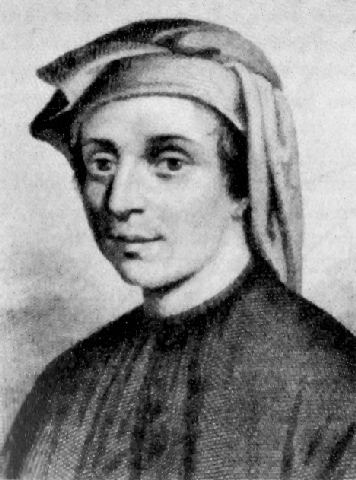
\includegraphics[width=0.5\textwidth]{Fibonacci.jpg}
    \caption{Leonardo da Pisa (1170-1240), auch Fibonacci genannt}
    \label{fig:Fibonacci}
\end{figure}

\clearpage

\begin{aufgabe}{aufgabe:0306}
Implementieren Sie eine Python-Funktion \pythoninline{def fibonacci(n)}, welche für gegebenes $n\in\N$ das $n$-te Glied der Fibonacci-Folge rekursiv berechnet. Geben Sie schliesslich die ersten $25$ Glieder der Fibonacci-Folge aus.
\end{aufgabe}
\begin{antwort}{aufgabe:0306}
\begin{lstlisting}[language=Python,caption=rekursive Berechnung der Fibonacci-Folge]
def fibonacci(n):
    if n <= 1:
        return n
    else:
        return fibonacci(n-1) + fibonacci(n-2)
\end{lstlisting}
\noindent
Die ersten $25$ Glieder der Fibonacci-Folge lauten:
\begin{lstlisting}[language=Python,caption=Die ersten 25 Glieder der Fibonacci-Folge]
0
1
1
2
3
5
8
13
21
34
55
89
144
233
377
610
987
1597
2584
4181
6765
10946
17711
28657
46368
\end{lstlisting}
\end{antwort}

\begin{aufgabe}{aufgabe:0307}
Versuchen wir $F_{40}$ mit der Python-Funktion aus \cref{aufgabe:0306} zu berechnen, stellen wir fest, dass die Berechnung bereits recht lange dauert. Erklären Sie, warum die Berechnung der Glieder der Fibonacci-Folge mit Hilfe der \cref{definition:fibonacci} sehr aufwendig ist. Wie viele Funktionsaufrufe werden für die Berechnung von $F(5)$ benötigt? Wie viele für $F(10)$?
\end{aufgabe}

\begin{antwort}{aufgabe:0307}
Die rekursiv definierte Python-Funktion aus \cref{aufgabe:0306} berechnet viele Folgeglieder mehrfach und arbeitet somit sehr \enquote{verschwenderisch}. Beispielsweise werden bei der Berechnung von $F_{40}$ die Berechnungen von $F_{39}$ und $F_{38}$ aufgerufen. Doch zur Berechnung von $F_{39}$ muss nochmals $F_{38}$ berechnet werden, und so weiter. In \cref{fig:fibonacciBaum} wird gezeigt, welche Funktionsaufrufe für die rekursive Berechnung von $F(5)$ benötigt werden. Beachten Sie, dass beispielsweise der Wert fib(2) dreimal berechnet wird. Es ist klar, dass die Anzahl der benötigten Funktionsaufrufe (und somit sicherlich auch die benötigten Rechenoperationen) zur Berechnung von $F(n)$ mit wachsendem $n$ stark ansteigt. Jede Fibonacci-Zahl, ausser $F(1)$ und $F(2)$, löst jeweils zwei Funktionsaufrufe aus. Damit ist es nicht schwierig, einzusehen, dass die Anzahl $A(n)$ der Funktionsaufrufe mindestens so schnell wächst wie die Fibonacci-Folge. Die genaue Anzahl ist gegeben durch
\begin{align*}
    A(n) = 2F(n+1) - 1.
\end{align*}
In \cref{ch:Kapitel04} werden Sie sehen, dass die Fibonacci-Folge exponentiell wächst.
\begin{figure}[H]
\centering
\begin{forest}
sn edges/.style={for tree={
parent anchor=south, child anchor=north}},
sn edges
[fib(5)
[fib(4) [fib(3) [fib(2) [fib(1)] [fib(0)] ] [fib(1)] ] [fib(2) [fib(1)] [fib(0)] ]]  [fib(3) [fib(2) [fib(1)] [fib(0)] ] [fib(1)]]
]
\end{forest}
\caption{Die Anzahl Funktionsaufrufe für $F(5)$ ist 15.}
\label{fig:fibonacciBaum}
\end{figure}
\end{antwort}

\begin{aufgabe}{aufgabe:0358}
Überlegen Sie sich, wie Sie die ersten $30$ Glieder der Fibonacci-Folge \enquote{von Hand} berechnen würden. Verwenden Sie diese Intuition um eine Python-Funktion \pythoninline{def fibonacci_fast(n)} zu schreiben, welche für gegebenes $n\in\N$ das $n$-te Glied der Fibonacci-Folge deutlich schneller und auf nicht rekursive Weise berechnet. Berechnen Sie mit Hilfe dieser Funktion das Folgeglied $F_{100}$.
\end{aufgabe}
\begin{antwort}{aufgabe:0358}
Die folgende Python-Funktion startet zur Berechnung von $F_n$ bei den Startwerten $F_0$ und $F_1$ und berechnet \enquote{von unten her} nacheinander (man spricht in diesem Zusammenhang von \textit{iterativer Berechnung}) die Nachfolger. Dabei werden keine Berechnungen \enquote{verschwendet}.
\begin{lstlisting}[language=Python,caption=iterative Berechnung der Fibonacci-Folge]
def fibonacci_fast(n):
    # Startwerte
    f0 = 0
    f1 = 1
    if n == 0:
        return f0
    elif n == 1:
        return f1
    
    for k in range(n-1):
        f2 = f1 + f0
        # Update
        f0 = f1
        f1 = f2
    return f2
\end{lstlisting}
Mit Hilfe dieser Funktion berechnen wir (in sehr kurzer Zeit)
\begin{align*}
    F_{100} = 354224848179261915075.
\end{align*}
\end{antwort}

\begin{aufgabe}{aufgabe:0309}
(*) Wir bezeichnen für $n\in\N$ mit $F_n$ die $n$-te Fibonacci-Zahl. Betrachten Sie die Gleichung
\begin{align}\label{eq:sumfib}
    F_{n+2} = 1 + \sum_{k=0}^{n} F_k
\end{align}
für $n\in\N$.
\begin{aenum}
    \item Beschreiben Sie die Aussage von \cref{eq:sumfib} in Ihren eigenen Worten.
    \item Beweisen Sie \cref{eq:sumfib}.
\end{aenum}
\end{aufgabe}
\begin{antwort}{aufgabe:0309}
\begin{aenum}
    \item Die $(n+2)$-te Fibonacci-Zahl ist um $1$ grösser als die Summe der Fibonacci-Zahlen $F_0,\ldots, F_n$.
    \item Wir beweisen die Behauptung durch vollständige Induktion. Für $n = 0$ haben wir
    \begin{align*}
        1 + \sum_{k=0}^{0} F_k = 1 + F_0 = 1 + 0 = 1 = F_2.
    \end{align*}
    Wir gehen nun von der Induktionsvoraussetzung
    \begin{align*}
        F_{n+1} = 1 + \sum_{k=0}^{n-1} F_k
    \end{align*}
        aus und finden
        \begin{align*}
            &F_{n+2} = \\
            &F_n + F_{n+1} = \\
            &F_n + \lr{1 + \sum_{k=0}^{n-1}F_k} = \\
            &1 + \sum_{k=0}^{n} F_k.
        \end{align*}
\end{aenum}
\end{antwort}


\clearpage
\section{Technische Umsetzung rekursiver Programme}\label{technisch}
In diesem Abschnitt werden wir den Übergang von der rein mathematischen Betrachtung rekursiver Algorithmen zu deren technischen Umsetzung vollziehen. Dazu betrachten wir ein Beispiel eines eleganten rekursiven Algorithmus, welcher für eine gegebene natürliche Zahl $n$, sämtliche binären Strings der Länge $n$ ausgibt. Insbesondere sollte der Algorithmus für die gegebenen Eingaben in den folgenden Testfällen die angegebenen Ausgaben erzeugen:
\begin{lstlisting}[language=Python,caption=binäre Strings rekursiv ausgeben,numbers=none]
TESTFALL 0
Eingabe: n = 0
Ausgaben:

(es wird eine leere Zeile (leerer String) ausgegeben)
TESTFALL 1
Eingabe: n = 1
Ausgaben:
0
1
TESTFALL 2
Eingabe: n = 2
Ausgaben:
00
01
10
11
TESTFALL 3
Eingabe: n = 3
Ausgaben:
000
001
010
011
100
101
110
111
\end{lstlisting}
Sie sind gerne eingeladen, an dieser Stelle vorerst nicht weiterzulesen und den Algorithmus selber zu schreiben.

Unser Vorschlag für einen entsprechenden rekursiven Algorithmus ist in \cref{listing:binary} gegeben.
\begin{lstlisting}[language=Python,caption=binaryStrings,label=listing:binary]
def binaryStrings(n, w = ''):
    if n == 0:
        print(w)
        return
    binaryStrings(n-1, w + '0')
    binaryStrings(n-1, w + '1')
    #return # optional
\end{lstlisting}
Zur Vereinfachung und Konkretisierung der Beschreibung der technischen Realisation rekursiver Algorithmen, werden wir sämtliche Betrachtungen dieses Abschnitts auf den Algorithmus in \cref{listing:binary} beziehen. Der Algorithmus beginnt mit dem leeren String und baut alle gesuchten Strings durch systematisches \enquote{Anhängen} von Nullen und Einsen auf. Zur Abkürzung schreiben wir anstelle von \verb|binaryString(...)| im Folgenden \verb|f(...)|.

\noindent
Betrachten wir den Aufruf \verb|f(2,'')| um alle Strings der Länge $2$ auszugeben. Die Arbeitsschritte, welche der Funktionsaufruf \verb|f(2,'')| einleitet, sind in \cref{fig:binary} dargestellt. Die \textcolor{Green!55}{grünen} Knoten stellen Funktionsaufrufe (Aufrufe von \verb|f|) dar. Die \textcolor{Gold!85}{goldenen} Knoten stellen Aufrufe der Python-Funktion \verb|print| dar. Beim Schritt mit Nummer $\textcolor{Blue}{0}$ erfolgt der anfängliche Aufruf \verb|f(2,'')|. In diesem Aufruf wird in Programmzeile $5$ der Funktionsaufruf \verb|f(1,'0')| ausgelöst (Schritt $\textcolor{Blue}{1}$). Beachten Sie, dass der ursprüngliche Aufruf \verb|f(2,'')| seine Arbeit noch nicht abgeschlossen hat! In Programmzeile $5$ des Funktionsaufrufs \verb|f(1,'0')| wird nun der Aufruf \verb|f(0,'00')| ausgelöst. In diesem Aufruf ist die \verb|if|-Bedingung auf Programmzeile $2$ erfüllt, sodass die Ausgabe \verb|print('00')| erfolgt (Schritt $3$) und der \verb|return| Aufruf auf Programmzeile $4$ erfolgt. Der Aufruf \verb|f(0,'00')| ist beendet und er springt zurück zum Aufruf \verb|f(1,'0')| (Schritt $\textcolor{Red}{4}$). Der Funktionsaufruf \verb|f(1,'0')| kann nun (endlich) zu Programmzeile $6$ gelangen und den Aufruf \verb|f(0,'01')| auslösen (Schritt $\textcolor{Blue}{5}$).

\begin{figure}[H]
\centering
\begin{tikzpicture}[scale=0.7, every node/.style={scale=0.7}, 
    ->, >=stealth', shorten >=1pt, auto, node distance=2.5cm, semithick]
    \tikzstyle{every state}=[fill=Green!10,draw=black,text=black]
    
    \node[state] (f2-leer) {\verb|f(2,'')|};
    \node[state] (f1-0) [below left=1.5cm and 3.4cm of f2-leer] {\verb|f(1,'0')|};
    \node[state] (f0-00) [below left=1.5cm and 1cm of f1-0] {\verb|f(0,'00')|};
    \node[state,fill=Gold!15] (p-00) [below=1.5cm of f0-00] {\verb|print('00')|};
    \node[state] (f0-01) [below right=1.5cm and 1cm of f1-0] {\verb|f(0,'01')|};
    \node[state,fill=Gold!15] (p-01) [below=1.5cm of f0-01] {\verb|print('01')|};
    \node[state] (f1-1) [below right=1.5cm and 3.4cm of f2-leer] {\verb|f(1,'1')|};
    \node[state] (f0-10) [below left=1.5cm and 1cm of f1-1] {\verb|f(0,'10')|};
    \node[state,fill=Gold!15] (p-10) [below=1.5cm of f0-10] {\verb|print('10')|};
    \node[state] (f0-11) [below right=1.5cm and 1cm of f1-1] {\verb|f(0,'11')|};
    \node[state,fill=Gold!15] (p-11) [below=1.5cm of f0-11] {\verb|print('11')|};

    \node[above=0.2cm of f2-leer] {\textcolor{Blue}{$0$ (anfänglicher Aufruf)}};

    \path   (f2-leer) edge [bend left, sloped, midway, above, Blue] node {$1$} (f1-0)
            (f1-0) edge [bend left, sloped, midway, above, Blue] node {$2$} (f0-00)
            (f0-00) edge [left, dashed] node {$3$} (p-00)
            (f0-00) edge [bend left, sloped, midway, above, Red] node {$4$} (f1-0)
            (f1-0) edge [bend left, sloped, midway, above, Blue] node {$5$} (f0-01)
            (f0-01) edge [left, dashed] node {$6$} (p-01)
            (f0-01) edge [bend left, sloped, midway, above, Red] node {$7$} (f1-0)
            (f1-0) edge [bend left, sloped, midway, above, Red] node {$8$} (f2-leer)

            (f2-leer) edge [bend left, sloped, midway, above, Blue] node {$9$} (f1-1)
            (f1-1) edge [bend left, sloped, midway, above, Blue] node {$10$} (f0-10)
            (f0-10) edge [left, dashed] node {$11$} (p-10)
            (f0-10) edge [bend left, sloped, midway, above, Red] node {$12$} (f1-1)
            (f1-1) edge [bend left, sloped, midway, above, Blue] node {$13$} (f0-11)
            (f0-11) edge [left, dashed] node {$14$} (p-11)
            (f0-11) edge [bend left, sloped, midway, above, Red] node {$15$} (f1-1)
            (f1-1) edge [bend left, sloped, midway, above, Red] node {$16$} (f2-leer)
    ;   
\end{tikzpicture}
\caption{Schematische Darstellung der Arbeitsschritte zur rekursiven Ausgabe aller binären Strings der Länge $2$.}
\label{fig:binary}
\end{figure}
\noindent
Erst nachdem auch \verb|f(0,'01')| seine Arbeit beendet hat (Schritte $6$ und $\textcolor{Red}{7}$), erreicht der Aufruf \verb|f(1,'0')| seine Programmzeile $7$ und springt zurück zum ursprünglichen Aufruf \verb|f(2,'')| (Schritt $\textcolor{Red}{7}$). Dieser erreicht nun Programmzeile $6$ und ruft \verb|f(1,'1')| auf (Schritt $\textcolor{Blue}{9}$). Die Schritte in dieser \enquote{rechten} Hälfte von \cref{fig:binary} lassen sich nun analog beschreiben. Erst nach der Rückgabe des Aufrufs \verb|f(1,'1')| in Schritt $\textcolor{Red}{16}$ kann schliesslich der ursprüngliche Aufruf \verb|f(2,'')| seine Arbeit beenden.

\clearpage
\begin{myBox}[Wie werden rekursive Programme in Computern realisiert?]{-}
In Computern wird für jeden Funktionsaufruf (Prozedur) ein Abschnitt im Speicher angelegt. Dieser Speicherabschnitt wird \textit{Stack-Frame} genannt. Darin darf die Funktion Speicherplatz zum Beispiel für lokale Variablen belegen. Deshalb benötigen rekursive Programme mit zahlreichen rekursiven Aufrufen viel Platz im Speicher.

Ruft eine Prozedur \verb|A| eine andere Prozedur \verb|B| auf, so wird im Stack-Frame von Prozedur \verb|B| eine sogenannte \textit{Rücksprung-Adresse} gespeichert. Diese Adresse gibt an, wo im Speicher die Prozedur \verb|A| beginnt. Dadurch wird ermöglicht, dass Prozedur \verb|B| zu Prozedur \verb|A| \enquote{zurückspringen} kann (\textit{jump and link}). Mehr Details bezüglich der Funktionsweise von Computern und rekursiven Programmen finden Sie in den hervorragenden Texten \cite{Malvino} und \cite{Sauter}.
\end{myBox}

\clearpage
\shipoutAnswer % Rekursion
        \part{Ausgewählte rekursive Probleme und Algorithmen}
        \chapter{Binäre Strings ohne aufeinanderfolgende Einsen (*)}\label{ch:Kapitel04}
In \cref{listing:binary} haben wir bereits eine Python-Funktion geschrieben, welche rekursiv alle binären Strings einer gegebenen Länge $n$ ausgibt. Es wird sich ein interessanter und überraschender Zusammenhang zur Fibonacci-Folge ergeben, wenn wir nicht alle binären Strings der Länge $n$ ausgeben, sondern nur die binären Strings der Länge $n$, welche nicht das Muster $11$ (Eins-Eins) enthalten. Wir interessieren uns also nur für die binären Strings, welche nicht zwei aufeinanderfolgende Einsen enthalten.
\begin{aufgabe}{aufgabe:0401}
Ändern Sie \cref{listing:binary} dahingehend ab, dass für gegebenes $n\in\N$ genau die binären Strings der Länge $n$ ohne aufeinanderfolgende Einsen ausgegeben werden. Beginnen Sie auch hier wieder mit dem leeren String und bauen Sie die gesuchten Strings rekursiv auf. Geben Sie Ihrer Funktion die Signatur

\pythoninline{print_binary_without_11(n, w = '')}.
\begin{lstlisting}[language=Python,caption=binäre Strings ohne 11 rekursiv ausgeben,numbers=none]
TESTFALL 0
Eingabe: n = 0, Ausgaben:

(es wird eine leere Zeile (leerer String) ausgegeben)
TESTFALL 1
Eingabe: n = 1, Ausgaben:
0
1
TESTFALL 2
Eingabe: n = 2, Ausgaben:
00
01
10
TESTFALL 3
Eingabe: n = 3, Ausgaben:
000
001
010
100
101
\end{lstlisting}
\end{aufgabe}
\begin{antwort}{aufgabe:0401}
\begin{lstlisting}[language=Python,caption=Binäre Strings ohne $11$]
def print_binary_without_11(n, w = ''):
    if n == 0:
        print(w)
        return
    
    if len(w) == 0 or  w[-1] != '1':
        print_binary_without_11(n-1, w + '0')
        print_binary_without_11(n-1, w + '1')
    else:
        print_binary_without_11(n-1, w + '0')
\end{lstlisting}
\end{antwort}

\clearpage


\section{Anzahl der binären Strings ohne 11}
Sei $n$ eine natürliche Zahl. Wir bezeichnen mit $L_n$ die Menge aller binären Strings der Wörter $n$, die nicht den Teilstring $11$ enthalten und setzen $N(n) = \abs{L_n}$. Wir wollen $N(n)$, also die Anzahl der Elemente in $L_n$, rekursiv bestimmen. Offensichtlich gilt $N(0) = 1$, denn nur der leere String hat die Länge $0$ und dieser enthält nicht den Teilstring $11$. Des Weiteren gilt $N(1) = 2$, da die Strings $0$ und $1$ beide nicht den Teilstring $11$ enthalten.

\begin{aufgabe}{aufgabe:0402}
Vervollständigen Sie \cref{table:Nn}.
    \begin{table}[H]
        \begin{center}
        \begin{tabular}{c|c}
        $n$ & $N(n)$ \\ \hline
        $0$ & $1$ \\
        $1$ & $2$ \\ 
        $2$ & $3$ \\
        $3$ & $5$ \\
        $4$ & \\
        $5$ & \\ 
        \end{tabular}
        \end{center}
        \caption{Tabelle für $N(n)$}
        \label{table:Nn}
    \end{table}
\end{aufgabe}
\begin{antwort}{aufgabe:0402}
    \begin{table}[H]
        \begin{center}
        \begin{tabular}{c|c}
        $n$ & $N(n)$ \\ \hline
        $0$ & $1$ \\
        $1$ & $2$ \\ 
        $2$ & $3$ \\
        $3$ & $5$ \\
        $4$ & $8$ \\
        $5$ & $13$ \\ 
        $6$ & $21$ \\
        $7$ & $34$ \\
        $8$ & $55$ \\
        \end{tabular}
        \end{center}
        \caption{ausgefüllte Tabelle für $N(n)$}
        \label{table:Nncompleted}
    \end{table}
\end{antwort}
Betrachten wir nun einen binären String $w$ der Länge $n+1$ mit $n\geq 1$. Angenommen $w$ liegt in $L_{n+1}$, dann enthält offensichtlich auch keiner der Teilstrings von $w$ das Muster $11$. Dann können wir $w\in L_{n+1}$ schreiben als
\begin{align*}
    w = xab,
\end{align*}
wobei $x\in L_{n-1}$ und $a,b\in\lrc{0,1}$.

\begin{aufgabe}{aufgabe:0403}
Wir nehmen an, dass die Anzahlen $N(n)$ und $N(n-1)$ für ein $n$ mit $n\geq 1$ bereits bekannt sind. Wir haben soeben begründet, dass wir $w$ in $L_{n+1}$ schreiben können als
\begin{align*}
    w = xab,
\end{align*}
wobei $x\in L_{n-1}$ und $a,b\in\lrc{0,1}$. Unterscheiden Sie nun zwei Fälle $b = 0$ und $b = 1$ für das Symbol $b$. Drücken Sie $N(n+1)$ durch $N(n)$ und $N(n-1)$ aus.
\end{aufgabe}
\begin{antwort}{aufgabe:0403}
    Wir unterscheiden zwei möglichen Fälle für das Symbol $b$.
    \begin{itemize}
        \item Falls $b = 0$, dann hat $w$ die Form $w = xab = xa0$. Da $b = 0$ ist, kann $a$ sowohl $0$ als auch $1$ sein (es gibt keine Einschränkung für $a$). Dann hat also $w$ die Form
        \begin{align*}
            w = \underbrace{xa}_{=:y}0 = y0,
        \end{align*}
        wobei $y$ ein beliebiger String aus $L_n$ sein darf und $L_n$ enthält $N(n)$ Elemente.
        \item  Falls $b = 1$, dann muss $a = 0$ gelten. Für $x$ ist dann aber ein beliebiger String aus $L_{n-1}$ möglich und $L_{n-1}$ enthält $N(n-1)$ Elemente.
    \end{itemize}
    Da für $b$ genau zwei Fälle möglich sind und diese Fälle keine \enquote{Überlappung} aufweisen, können wir die jeweiligen Anzahlen addieren und erhalten die Gleichung
    \begin{align}\label{eq:rekkurenz}
        N(n+1) = N(n) + N(n-1).
    \end{align}
    Dies sieht aber genauso aus wie die rekursive Definition der Fibonacci-Folge! Aufgrund der bereits gefundenen Anfangsbedingungen $N(0) = 1$ und $N(1) = 2$, muss die gewöhnliche Fibonacci-Folge \enquote{verschoben} werden und wir sehen
    \begin{align*}
        N(n) = F(n+2).
    \end{align*}
\end{antwort}

\section{Explizite und rekursive Darstellungen von Folgen}
Wir betrachten die rekursiv definierte Folge
\begin{align*}
    a_0 &= -1, \\
    a_{n+1} &= a_n + 4.
\end{align*}
Ein Folgenglied mit grösserem Index, wie zum Beispiel $a_{5000}$, zu berechnen, ist recht mühsam. In dieser rekursiven Darstellung müssten für die Berechnung von 
$a_{5000}$ nämlich alle Glieder $a_{1}, a_{2}, \ldots, a_{4999}$ zuerst bestimmt werden. Wie können wir späte Folgenglieder (mit hohen Indizes) effizienter berechnen? Die folgende \cref{aufgabe:0404} wird sich mit dieser Frage beschäftigen.

\begin{aufgabe}{aufgabe:0404}
Finden Sie eine \enquote{Formel}, welche $a_n$ mit lediglich einer Multiplikation und einer Addition berechnet, ohne zuerst die Vorgänger $a_{1}, a_{2}, \ldots, a_{n}$ bestimmen zu müssen. Berechnen Sie mit Hilfe dieser Formel das Folgenglied $a_{5000}$.
\end{aufgabe}
\begin{antwort}{aufgabe:0404}
Wir bemerken, dass das nachfolgende Folgenglied um 4 grösser ist als sein Vorgänger. Damit ist $a_n$ genau $4n$ grösser als $a_0$ und wir erhalten
\begin{align*}
    a_n = a_0 + 4n = 4n - 1.
\end{align*}
Nun finden wir $a_{5000} = 4\cdot 5000 - 1 = 19999$.
\end{antwort}
Die in \cref{aufgabe:0404} gefundene (nicht rekursive) Darstellung von $a_n$ wird \tib{explizite Darstellung}\index{Folge!explizite Darstellung einer} von $a_n$ genannt.

\begin{aufgabe}{aufgabe:0405}
Beweisen Sie durch vollständige Induktion, dass $a_n = n^2 -2n$ eine explizite Darstellung der rekursiv definierten Folge
\begin{align*}
    a_0 = 0, \quad a_{n} = a_{n-1} + 2n - 3
\end{align*}
für $n\in\Nunit$ ist.
\end{aufgabe}
\begin{antwort}{aufgabe:0405}
Wegen $a_0 = 0^2 - 2\cdot 0 = 0$ ist der Induktionsanfang gezeigt. Angenommen die Aussage gilt für $n$. Wir zeigen, dass sie auch für $n+1$ gilt, dass also $a_{n+1} = (n+1)^2 - 2(n+1) = n^2 - 1$. In der Tat ist
\begin{align*}
    a_{n+1} = a_n + 2(n+1) - 3 = n^2 - 2n + 2(n+1) - 3 = n^2 - 1.
\end{align*}
\end{antwort}
Die rekursive Darstellung \cref{eq:rekkurenz} ist nicht geeignet, um $N(n)$ für grosse Werte von $n$ zu berechnen. Die Fibonacci-Folge wurde bereits im  Jahr 1202 von Leonardo da Pisa verwendet, um das Wachstum einer Kaninchenpopulation zu beschreiben. Dennoch gelang es (höchst wahrscheinlich) erst in der ersten Hälfte des 18. Jahrhunderts, eine explizite Darstellung dieser wichtigen Folge zu finden. Diese Darstellung zu finden ist also alles andere als einfach. Diese explizite Darstellung ist als \textit{Formel von Moivre-Binet} bekannt und besagt
\begin{align}\label{eq:binet}
    F(n) = \frac{\varphi^n - (1-\varphi)^n}{\sqrt{5}},
\end{align}
wobei $\varphi := \frac{1+\sqrt{5}}{2}$.

\cref{eq:binet} enthält die irrationale Zahl $\sqrt{5}$. Ist es nicht erstaunlich, dass $F(n)$ für alle $n\in\N$ eine natürliche Zahl ist? In der anspruchsvollen \cref{aufgabe:0477} haben Sie die Gelegenheit zu beweisen, dass die Formel von Moivre-Binet tatsächlich die Fibonacci-Zahlen berechnet (und somit ausschliesslich natürliche Zahlen generiert).

\begin{aufgabe}{aufgabe:0478}
Berechnen Sie $F(0)$ und $F(1)$ mit Hilfe von \cref{eq:binet}. Überzeugen Sie sich, dass $F(0)$ und $F(1)$ die ersten beiden Fibonacci-Zahlen und somit insbesondere natürliche Zahlen sind.
\end{aufgabe}
\begin{antwort}{aufgabe:0478}
Wir berechnen
\begin{align*}
    F(0) &= \frac{\varphi^0-\alpha^0}{\sqrt{5}} = 0 = F_0, \\
    F(1) &= \frac{\varphi^1-\alpha^1}{\sqrt{5}} = \frac{\varphi-(1-\varphi)}{\sqrt{5}} = \frac{2\varphi-1}{\sqrt{5}} = \frac{1+\sqrt{5}-1}{\sqrt{5}} = 1 = F_1.
\end{align*}
\end{antwort}

\clearpage
\begin{aufgabe}{aufgabe:0477}
(!) Beweisen Sie durch starke Induktion, dass die $n$-te Fibonacci-Zahl $F_n$ durch den Ausdruck $F(n)$ in \cref{eq:binet} gegeben ist. 

\noindent
Hinweis:
\begin{itemize}
    \item Definieren Sie zuerst
    \begin{align*}
        \alpha := 1-\varphi
    \end{align*}
    und beachten Sie, dass
    \begin{align*}
        \alpha = 1-\varphi = 1 - \frac{1+\sqrt{5}}{2} = \frac{2 - 1 - \sqrt{5}}{2} =  \frac{1-\sqrt{5}}{2}.
    \end{align*}
    \item Beweisen und verwenden Sie nun die beiden Gleichungen
    \begin{align*}
        \varphi^2 &= 1+\phi,\\
        \alpha^2 &= 1+\alpha.
    \end{align*}
\end{itemize}
\end{aufgabe}
\begin{antwort}{aufgabe:0477}
Wir beweisen zuerst die Gleichungen aus dem Hinweis:
\begin{align*}
    \varphi^2 &= \lr{\frac{1+\sqrt{5}}{2}}^2 = \frac{6+2\sqrt{5}}{4} = 1 + \frac{1+\sqrt{5}}{2} = 1 + \varphi, \\
    \alpha^2 &= \lr{\frac{1-\sqrt{5}}{2}}^2 = \frac{6-2\sqrt{5}}{4} = 1 + \frac{1-\sqrt{5}}{2} = 1 + \alpha.
\end{align*}
In \cref{aufgabe:0478} haben wir bereits die Korrektheit der Aussage für $n=0$ und $n=1$ gezeigt. Sei nun die Aussage für ein $n\in\Nunit$ wahr.
\begin{align*}
    F_{n+1} & \stackrel{\text{Definition von $F_{n+1}$}}{=} F_n + F_{n-1} = \\
    &\frac{\varphi^{n}-\alpha^{n}}{\sqrt{5}} + \frac{\varphi^{n-1}-\alpha^{n-1}}{\sqrt{5}} = \\
    &\frac{\varphi^{n} + \varphi^{n-1} - \lr{\alpha^{n}+\alpha^{n-1}}}{\sqrt{5}} = \\
    &\frac{\lr{\varphi + 1}\varphi^{n-1} - \lr{\lr{\alpha + 1}\alpha^{n-1}}}{\sqrt{5}} = \\
    &\frac{\varphi^2\varphi^{n-1} - \alpha^2\alpha^{n-1}}{\sqrt{5}} = \\
    &\frac{\varphi^{n+1}-\alpha^{n+1}}{\sqrt{5}} = \frac{\varphi^{n+1}-(1-\varphi)^{n+1}}{\sqrt{5}} = F(n+1)
\end{align*}
\end{antwort}

\bemerkung{bemerkung:moivre}{
Die Formel von Moivre-Binet enthält Terme, welche Computer aufgrund ihrer (nur) endlichen Arithmetik, nicht exakt darstellen können. Eine einfache Beobachtung macht die Formel aber auch für die Berechnung in endlicher Arithmetik gut zugänglich. Wir schreiben zuerst
\begin{align*}
    F(n) = \frac{\varphi^n - (1-\varphi)^n}{\sqrt{5}} = \textcolor{blue}{\frac{\varphi^n}{\sqrt{5}}} - \textcolor{Green}{\frac{(1-\varphi)^n}{\sqrt{5}}}.
\end{align*}
Die Fibonacci-Zahl $F_n$ unterscheidet sich von der Zahl $\textcolor{blue}{\frac{\varphi^n}{\sqrt{5}}}$ also lediglich um den Term $\textcolor{Green}{\frac{(1-\varphi)^n}{\sqrt{5}}}$. Doch wie gross ist dieser Term? Für den Exponenten $n=0$ reduziert er sich auf
\begin{align*}
    \abs{\frac{1-\varphi}{\sqrt{5}}}.
\end{align*}
Wegen $\abs{1-\varphi} < 1$ gilt
\begin{align*}
    \abs{\frac{1-\varphi}{\sqrt{5}}} < \frac{1}{\sqrt{5}} < \frac{1}{2}.
\end{align*}
Was ändert sich aber, wenn wir allgemeine Exponenten $n\in\N$ zulassen? Tatsächlich gilt: Je grösser der Exponent ist, desto kleiner ist der Term! Aufgrund der Abschätzung $\abs{1-\varphi} < 1$ wissen wir nämlich, dass die geometrische Folge
\begin{align*}
    \abs{\textcolor{Green}{\frac{(1-\varphi)^n}{\sqrt{5}}}} = \frac{1}{\sqrt{5}}\abs{(1-\varphi)^n} = \frac{1}{\sqrt{5}}\abs{1-\varphi}^n
\end{align*}
strikt monoton fallend ist. Damit gilt also für alle natürlichen Exponenten $n\in\N$
\begin{align*}
    \abs{\textcolor{Green}{\frac{(1-\varphi)^n}{\sqrt{5}}}} < \frac{1}{2}. 
\end{align*}
Wir haben somit nachgewiesen, dass
\begin{alignat*}{2}
    \textcolor{blue}{\frac{\varphi^n}{\sqrt{5}}} - \frac{1}{2} &< \underbrace{\textcolor{blue}{\frac{\varphi^n}{\sqrt{5}}} - \textcolor{Green}{\frac{(1-\varphi)^n}{\sqrt{5}}}}_{F_n} &&< \textcolor{blue}{\frac{\varphi^n}{\sqrt{5}}} + \frac{1}{2} \iff \\
    - \frac{1}{2} &< \quad\; F_n - \textcolor{blue}{\frac{\varphi^n}{\sqrt{5}}} &&< \frac{1}{2},
\end{alignat*}
oder anders geschrieben:
\begin{align*}
    \abs{F_n-\textcolor{blue}{\frac{\varphi^n}{\sqrt{5}}}} < \frac{1}{2}.
\end{align*}
Der Abstand von $\textcolor{Blue}{\varphi^n/\sqrt{5}}$ zu der ganzen Zahl $F_n$ ist also kleiner als $1/2$. Es liegt damit keine ganze Zahl so nahe bei $\textcolor{Blue}{\varphi^n/\sqrt{5}}$ wie $F_n$. Die $n$-te Fibonacci-Zahl $F_n$ entspricht somit $\textcolor{Blue}{\varphi^n/\sqrt{5}}$, gerundet auf die nächste ganze Zahl:
\begin{align}\label{eq:moivrecomp}
    F_n = \lrs{\textcolor{blue}{\frac{\varphi^n}{\sqrt{5}}}}, \quad\text{für alle } n\in\N.
\end{align}
Damit ist nun auch klar ersichtlich, dass die Fibonacci-Folge exponentiell wächst!
}

\begin{aufgabe}{aufgabe:0406}
Verwenden Sie die Formel von Moivre-Binet um eine explizite Darstellung von $N(n)$ zu finden und schreiben Sie eine Python-Funktion \pythoninline{def N(n)}, welche $N(n)$ für gegebenes $n\in\N$ berechnet. Verwenden Sie dazu \cref{eq:moivrecomp}.
\end{aufgabe}
\begin{antwort}{aufgabe:0406}
Wir haben bereits festgestellt, dass
\begin{align*}
    N(n) = F(n+2) = \frac{\varphi^{n+2}-(1-\varphi)^{n+2}}{\sqrt{5}}
\end{align*}
mit $\varphi := \frac{1+\sqrt{5}}{2}$ gilt. Das entsprechende Programm lautet:
\begin{lstlisting}[language=Python]
import math

def N(n):
    sqrt5 = math.sqrt(5)
    phi = (1 + sqrt5)/2
    return int(round(phi**(n+2)/sqrt5))
\end{lstlisting}
\end{antwort}

\clearpage
\shipoutAnswer % Binäre Strings ohne aufeinanderfolgende Nullen
        \chapter{Sortieren (*)}\label{ch:Kapitel05}

Eines der häufigsten algorithmischen Probleme ist das \textit{Sortieren}.
\begin{definition}[Sortierproblem]{definition:Sortierproblem}
    Sei $S$ eine Menge deren Elemente durch die Relation $\leq$ verglichen werden können ($\leq$ heisst dann \textit{totale Ordnung} auf $S$). Das \tib{Sortierproblem}\index{Sortierproblem} lautet dann:
    \begin{description}
        \item[Eingabe:] Eine endliche Folge von $n\in\Nunit$ Elementen $a_1,a_2,\ldots,a_n$ aus $S$.
        \item[Ausgabe:] Eine Umordnung $a_1', a_2', \ldots, a_n'$ der Eingabe, sodass $a_1'\leq a_2' \leq \ldots \leq a_n'$ (die Elemente der Eingabe sind nun aufsteigend sortiert).
    \end{description}
\end{definition}
\cref{fig:bsp1,fig:bsp2} zeigen zwei einfache Beispiele von Eingaben und entsprechenden Ausgaben des Sortierproblems.

\begin{figure}[H]
    \def\lvld{1.2}                  % Choose level distance
    \pgfmathsetmacro\shft{-6*\lvld} % Calculate the yshift for the green tree
    \centering
\begin{tikzpicture}[level distance=\lvld cm,
                        level 1/.style={sibling distance=4cm},
                        level 2/.style={sibling distance=2cm},
                        level 3/.style={sibling distance=1cm},
                        edgedown/.style={edge from parent/.style={draw=red,thick,-latex}},
                        edgeup/.style={edge from parent/.style={draw=green!50!black,thick,latex-}}
                        ]
        \node[block=7,label={Eingabe}] (A) {3 \nodepart{two} 2 \nodepart{three} 0 \nodepart{four} 3 \nodepart{five} 9 \nodepart{six}8 \nodepart{seven}1}
            [grow=down,edgedown];
        \node[block=7,below=1cm of A,label={Ausgabe}] (B) {0 \nodepart{two} 1 \nodepart{three} 2 \nodepart{four} 3 \nodepart{five} 3 \nodepart{six}8 \nodepart{seven}9}
            [grow=down,edgedown];
\end{tikzpicture}
    \caption{Eingabe und Ausgabe eines kleinen Sortierproblems mit ganzen Zahlen}
    \label{fig:bsp1}
\end{figure}

\begin{figure}[H]
    \def\lvld{1.2}                  % Choose level distance
    \pgfmathsetmacro\shft{-6*\lvld} % Calculate the yshift for the green tree
    \centering
\begin{tikzpicture}[level distance=\lvld cm,
                        level 1/.style={sibling distance=4cm},
                        level 2/.style={sibling distance=2cm},
                        level 3/.style={sibling distance=1cm},
                        edgedown/.style={edge from parent/.style={draw=red,thick,-latex}},
                        edgeup/.style={edge from parent/.style={draw=green!50!black,thick,latex-}}
                        ]
        \node[block=5,label={Eingabe}] (A) {$r$ \nodepart{two} $e$ \nodepart{three} $a$ \nodepart{four} $o$ \nodepart{five} $n$}
            [grow=down,edgedown];
        \node[block=5,below=1cm of A,label={Ausgabe}] (B) {$a$ \nodepart{two} $e$ \nodepart{three} $n$ \nodepart{four} $o$ \nodepart{five} $r$}
            [grow=down,edgedown];
\end{tikzpicture}
    \caption{Eingabe und Ausgabe eines kleinen Sortierproblems mit Kleinbuchstaben des lateinischen Alphabets. Dabei wurde die übliche alphabetische Ordnung $a\leq b\leq \ldots \leq z$ verwendet.}
    \label{fig:bsp2}
\end{figure}

\section{Sortieren mit dem \textit{merge sort} Algorithmus}
Natürlich ist das Bedürfnis nach schnellen Algorithmen besonders gross, falls diese Probleme lösen, die zeitkritisch sind und häufig auftreten. Mittlerweile sind viele Sortieralgorithmen bekannt. Ein berühmter Vertreter dieser Algorithmen ist \textit{merge sort}. Der Algorithmus \textit{merge sort} arbeitet rekursiv. Dabei macht er insbesondere von der Tatsache Gebrauch, dass sich zwei sortierte Listen recht effizient zu einer ebenfalls sortierten Liste zusammenfügen lassen. Es seien also zwei jeweils \textbf{bereits sortierte} Listen \pythoninline{L} und \pythoninline{R} gegeben. Diese Listen besitzen die Längen (Anzahl von Elementen) \pythoninline{len(L)} und \pythoninline{len(R)}. Es ist nun nicht besonders aufwändig, die beiden Listen \pythoninline{L} und \pythoninline{R} zu einer neuen \textbf{sortierten} Liste \pythoninline{M} der Länge \pythoninline{len(L) + len(R)} zu vereinen (englisch: \textit{to merge}).

\begin{aufgabe}{aufgabe:0501}
Angenommen wir haben zwei jeweils \textbf{bereits sortierte} Listen \pythoninline{L} und \pythoninline{R} gegeben. Schreiben Sie eine Python Funktion \pythoninline{merge(L,R)}, welche \pythoninline{L} und \pythoninline{R} zu einer einzigen sortierten Liste vereint. Ihre Funktion soll unbedingt Gebrauch von der Tatsache machen, dass \pythoninline{L} und \pythoninline{R} bereits sortiert sind.
\begin{lstlisting}[language=Python,caption=Testfälle für die Funktion \pythoninline{merge}.,numbers=none]
Testfall 0
Eingabe: L = [8, 12, 17], R = []
Ausgabe: [8, 12, 17]

Testfall 1
Eingabe: L = [2, 5, 13], R = [1, 2, 3, 7, 15, 20]
Ausgabe: [1, 2, 2, 3, 5, 7, 13, 15, 20]

Testfall 2
Eingabe: L = [1,10,100,1000], R = [0,5,50]
Ausgabe: [0, 1, 5, 10, 50, 100, 1000]
\end{lstlisting}
Ihre Funktion braucht nicht zu überprüfen, ob \pythoninline{L} und \pythoninline{R} tatsächlich sortiert sind.
\end{aufgabe}
\begin{antwort}{aufgabe:0501}
\begin{lstlisting}[language=Python,caption=Implementation der Funktion \pythoninline{merge}.,label=listing:merge]
def merge(L,R):
    # L und R sind jeweils bereits sortierte Listen

    # M wird am Ende len(L) + len(R) viele Elemente haben
    # und eine sortierte Liste sein
    M = [] # M ist zu Beginn einen leere Liste

    l = 0 # Laufindex innerhalb der Liste L
    r = 0 # Laufindex innerhalb der Liste R

    # solange weder L noch R vollständig durchlaufen wurden
    while (l < len(L)) and (r < len(R)):
        if L[l] <= R[r]:
            M.append(L[l])
            l = l + 1
        else:
            M.append(R[r])
            r = r + 1

    while l < len(L):
        M.append(L[l])
        l = l + 1
    while r < len(R):
        M.append(R[r])
        r = r + 1
    return M
\end{lstlisting}     
\end{antwort}

\begin{aufgabe}{aufgabe:0502}
Analysieren Sie den Algorithmus, welchen Sie in \cref{aufgabe:0501} geschrieben haben. Welche Laufzeit hat dieser Algorithmus in Abhängigkeit von \pythoninline{n = len(L) + len(R)}?
\end{aufgabe}

\begin{antwort}{aufgabe:0502}
Wir beziehen uns hier auf den Algorithmus in der Musterlösung zu \cref{aufgabe:0501}. Der Algorithmus besteht im Wesentlichen in einer Schleife über die summierte Länge
\begin{center}
    \pythoninline{n = len(L) + len(R)}
\end{center}
der beiden gegebenen Listen. Somit ist die Laufzeit gegeben durch $\Theta(n)$.
\end{antwort}

\noindent
Der \textit{merge sort} Algorithmus teilt eine zu sortierende Liste rekursiv so lange in zwei Teile, bis nur noch Listen der Länge 1 vorliegen. Offensichtlich ist jede Liste der Länge 1 bereits sortiert. Schliesslich werden bereits sortierte Listen mit Hilfe des \textit{merge} Algorithmus zu der gesuchten sortierten Liste zusammengefügt. Mit Hilfe der bereits in \cref{aufgabe:0501} erstellten Routine \textit{merge}, lässt sich der berühmte \textit{merge sort} Algorithmus in nur wenigen Zeilen in Python beschreiben. Eine mögliche Implementation ist in \cref{listing:mergesort} gegeben.
\begin{lstlisting}[language=Python,caption=Implementation der Funktion \pythoninline{merge_sort}.,label=listing:mergesort]
def merge_sort(A):
    # sortiert die Liste A
    if len(A) == 1: # Rekursionsanfang
        return A # Listen der Länge 1 sind schon sortiert

    # teile A in linke Hälfte und rechte Teile
    if len(A) % 2 == 0: # falls len(A) gerade ist
        middle = len(A) // 2
    else: # falls len(A) ungerade ist
        middle = (len(A) // 2) + 1
    L = merge_sort(A[:middle])
    R = merge_sort(A[middle:])
    return merge(L,R)
\end{lstlisting} 
Den \textit{merge sort} Algorithmus zu verstehen ist nicht einfach! Erfahrungsgemäss ist es sehr hilfreich, die einzelnen Schritte dieses Sortieralgorithmus für ein kleines Beispiel durchzugehen. Dazu haben wir die Schritte von \textit{merge sort} (\verb|ms|) beim Sortieren der Liste \pythoninline{[3,2,1]} in \cref{fig:mergesort} schematisch dargestellt. Mit \verb|m| wird natürlich der Algorithmus \textit{merge} bezeichnet. Die schematische Darstellung ist analog zu den Ausführungen in \cref{technisch} zu verstehen.
\begin{figure}[H]
    \centering
    \begin{tikzpicture}[scale=0.7, every node/.style={scale=0.7}, 
        ->, >=stealth', shorten >=1pt, auto, node distance=3.5cm, semithick]
        \tikzstyle{every state}=[fill=Green!10,draw=black,text=black]
        
        \node[state] (ms321) {\verb|ms([3,2,1])|};
        \node[state] (ms32) [below left=2.5cm and 1cm of ms321] {\verb|ms([3,2])|};
        \node[state] (ms3) [below left=1.5cm and 1cm of ms32] {\verb|ms([3])|};
        \node[state] (ms2) [below=1.5cm of ms32] {\verb|ms([2])|};
        \node[state,fill=Gold!15] (m32) [below right=1.5cm and 1cm of ms32] {\verb|m([3],[2])|};
        \node[state] (ms1) [below right=2.5cm and 1cm of ms321] {\verb|ms([1])|};
        \node[state,fill=Gold!15] (m231) [right=2.5cm of ms1] {\verb|m([2,3],[1])|};
        \node[above=0.2cm of ms321] {\textcolor{Blue}{$0$ (anfänglicher Aufruf)}};
    
        \path   (ms321) edge [bend left=15, sloped, midway, above, Blue] node {$1$} (ms32)
                (ms32) edge [bend left=15, sloped, midway, above, Blue] node {$2$} (ms3)
                (ms3) edge [bend left=15, sloped, midway, above, Red] node {$3$} (ms32)
                (ms32) edge [bend left=15, sloped, midway, right, Blue, rotate=-90] node {$4$} (ms2)
                (ms2) edge [bend left=15, sloped, midway, left, Red, rotate=-90] node {$5$} (ms32)
                (ms32) edge [bend left=15, sloped, midway, above, Blue] node {$6$} (m32)
                (m32) edge [bend left=15, sloped, midway, above, Red] node {$7$} (ms32)
                (ms32) edge [bend left, sloped, midway, above, Red] node {$8$} (ms321)
    
                (ms321) edge [bend left=15, sloped, midway, above, Blue] node {$9$} (ms1)
                (ms1) edge [bend left=15, sloped, midway, above, Red] node {$10$} (ms321)
                (ms321) edge [bend left=10, sloped, midway, above, Blue] node {$11$} (m231)
                (m231) edge [bend left=10, sloped, midway, above, Red] node {$12$} (ms321)
        ;
    \end{tikzpicture}
    \caption{schematische Darstellung der Arbeitsschritte von \textit{merge sort}}
    \label{fig:mergesort}
\end{figure}

\section{Analyse der Laufzeit von \textit{merge sort}}
Beachten Sie, dass der in \cref{listing:mergesort} gegebene Algorithmus durchaus in der Lage ist, Listen beliebiger Längen $n\in\N$ zu sortieren. Für die nachfolgenden Untersuchungen wollen wir aber annehmen, dass die Problemgrösse $n$ stets eine Zweierpotenz ist, also $n = 2^k$ für ein $k\in\N$. Ohne diese Vereinfachungen werden in den Untersuchungen diverse Auf- und Abrundeoperationen notwendig sein und die Darstellung wird technischer und weniger instruktiv. Zusätzlich möchten wir den trivialen Fall $n = 0$ als Problemgrösse ausschliessen. Die folgenden Betrachtungen sind inspiriert durch die entsprechenden Abschnitte in dem herausragenden Buch \cite{IntroductionAlgo}.

Die Laufzeit des \textit{merge sort} Algorithmus setzt sich aus drei einzelnen Teilen zusammen:
\begin{description}
  \item[Divide:] Dieser Teil berechnet lediglich die Mitte der zu sortierenden Liste. Dazu ist offensichtlich nur konstante Zeit $\Theta(1)$ notwendig.
  \item[Conquer:] Beim Aufruf des \textit{merge sort} Algorithmus mit Problemgrösse $n$, werden rekursiv \textcolor{Blue}{zwei} Teilprobleme (derselben Art) mit jeweils halber Grösse $\textcolor{Green}{n/2}$ aufgerufen. Dies trägt $\textcolor{Blue}{2}T(\textcolor{Green}{n/2})$ zur Laufzeit bei.
  \item[Combine:] Wie wir in \cref{aufgabe:0502} bereits festgestellt haben, benötigt \textit{merge sort} die lineare Zeit $\Theta(n)$ für die Vereinigung zweier Listen mit summierter Länge \pythoninline{n = len(L) + len(R)}.
\end{description}
Zusammengefasst ist die Laufzeit $T(n)$ von \textit{merge sort} im schlimmsten Fall also gegeben durch

\begin{align}\label{eq:rek1}
  T(n) = 
  \begin{cases}
    \Theta(1), &\text{falls $n = 1$,} \\
    2T(n/2) + \Theta(n), & \text{falls $n\geq 2$}.
  \end{cases}
\end{align}
\cref{eq:rek1} lässt sich natürlich schreiben als

\begin{align}\label{eq:rek2}
  T(n) = 
  \begin{cases}
    c_0, &\text{falls $n = 1$,} \\
    2T(n/2) + c_1n, & \text{falls $n\geq 2$}.
  \end{cases}
\end{align}
Diesen Ausdruck können wir mit der Definition $c := \max\lrc{c_0,c_1}$ sogar nochmals vereinfachen zu
\begin{align}\label{eq:rek3}
  T(n) = 
  \begin{cases}
    c, &\text{falls $n = 1$,} \\
    2T(n/2) + cn, & \text{falls $n\geq 2$},
  \end{cases}
\end{align}
da wir uns im Moment lediglich für eine obere Schranke für die Laufzeit $T(n)$ interessieren. Beachten Sie, dass \cref{eq:rek3} die Funktion $T$ (Laufzeit) rekursiv definiert. Gemäss \cref{satz:Rekursion} zum Prinzip der rekursiven Definition, existiert genau eine Funktion $T$, welche diese Gleichung erfüllt. Man bezeichnet solch eine rekursiv definierende Gleichung auch als \tib{Rekurrenzgleichung}\index{Rekurrenzgleichung}. 

Wir wollen nun die eindeutige Lösung von \cref{eq:rek3} durch intuitive Überlegungen finden. Betrachten Sie \cref{fig:mergesortBaum}.
\begin{itemize}
  \item In der \textcolor{Red}{obersten} \enquote{Etage} fallen die Kosten $cn$ für den \textit{merge} zu einer Liste der Länge $n$ an.
  \item In der \textcolor{Blue}{zweitobersten} \enquote{Etage} fallen die Kosten $cn/2 + cn/2 = cn$ für zwei \textit{merges} zu Listen der Längen $n/2$ an.
  \item Dies geht rekursiv so weiter.
  \item In der untersten \enquote{Etage} wird überall der Rekursionsanfang erreicht und wir haben $n$-mal die Kosten $T(1) = c$, also $cn$.
\end{itemize}
Diese Überlegung zeigt, dass jede \enquote{Etage} genau $cn$ zu den Gesamtkosten von \textit{merge sort} beiträgt. Nun stellt sich lediglich noch die Frage, wie viele \enquote{Etagen} der Baum in \cref{fig:mergesortBaum} hat. Diese Frage ist aber mit der Frage verwandt, wie häufig eine Zweierpotenz $2^k$ halbiert werden muss, bis das Resultat der Division durch 2 identisch zu 1 ist. Dies ist aber genau das, was uns der Logarithmus zur Basis zwei beantwortet. Der Faktor 2 ist
\begin{align*}
  \log_2(n) = \log_2\lr{2^k} = k
\end{align*}
mal in $n$ enthalten. Das ist die Anzahl Teilungen. Der Baum hat somit $\log_2(n) + 1$ viele \enquote{Etagen}. Die Laufzeit von \textit{merge sort} ist also
\begin{align*}
  cn\lr{\log_2(n) + 1}
\end{align*}
und somit $\Theta\lr{n\log(n)}$.

\begin{figure}[H]
    \centering
\begin{tikzpicture}[
    level/.style={sibling distance=40mm/#1},
    text=black,
    >=latex,
    font=\sffamily
    ]
% https://tex.stackexchange.com/questions/241232/creating-dots-lines-brackets-in-tree-with-tikz
\tikzset{
    edge from parent/.style={draw, thick, black},
    no edge from this parent/.style={
        every child/.append style={
        edge from parent/.style={draw=none}}},
    level 3/.style={yshift=5cm},
    level 4/.style={level distance=5mm} 
         }
  \node (z){\textcolor{Red}{$cn$}} 
  child {node (a) {\textcolor{Blue}{$cn/2$}}
    child {node  (b) {$cn/4$}
      child {node (b1) {$\vdots$}[no edge from this parent]
       child {node (b11) {$c$}}
      }
      child {node (b2) {$\vdots$}[no edge from this parent]
       child {node (b12) {$c$}}
      }
    }
    child {node (g) {$cn/4$}
      child {node (g1) {$\vdots$}[no edge from this parent]
       child {node (g11) {$c$}}
      }
      child {node (g2) {$\vdots$}[no edge from this parent]
       child {node (g12) {$c$}}
      }
    }
  }
    child {node (d) {\textcolor{Blue}{$cn/2$}}
      child {node  (e) {$cn/4$}
        child {node (e1) {$\vdots$}[no edge from this parent]
         child {node (e11) {$c$}}
        }
        child {node (e2) {$\vdots$}[no edge from this parent]
         child {node (e12) {$c$}}
        }
      }
      child {node (f) {$cn/4$}
        child {node (f1) {$\vdots$}[no edge from this parent]
         child {node (f11) {$c$}}
        }
        child {node (f2) {$\vdots$}[no edge from this parent]
         child {node (f12) {$c$}
        }
      }
  }
};

\node[left=5 of z]  (ln1) {$cn$}[no edge from this parent]
    child {node (ln2) {$cn$}[no edge from this parent]
        child {node (ln3) {$cn$}[no edge from this parent]
            child {node (ln4) {}[no edge from this parent]
                child {node (ln5) {$cn$}}}}};

\coordinate (cd1) at ($(f12)+(1,0)$);
\coordinate (nb1) at ($(g12)!.5!(e11)$);

\draw[black,thick,<->,] 
    (cd1) --node [fill=white] {$\log(n)$} (cd1|-z.east);

\draw[black,dashed,thick,->]    
    ($(z.west)+(-1em,0)$) -- (ln1);
\draw[black,dashed,thick,->]    
    ($(a.west)+(-1em,0)$) -- (ln2.east);
\draw[black,dashed,thick,->]    
    ($(b.west)+(-1em,0)$) -- (ln3);
\draw[black,dashed,thick,->]    
    ($(b11.west)+(-1em,0)$) -- (ln5);

\draw[Green!70!black,thick,decorate,decoration={brace,amplitude=10pt,mirror}] (b11.south west) --node [below=0.3cm] {$n$} (f12.south east);
\end{tikzpicture}
    \caption{Laufzeitanalyse von \textit{merge sort}}
    \label{fig:mergesortBaum}
\end{figure}

\begin{aufgabe}{aufgabe:0503}
Zeigen Sie mit Hilfe der vollständigen Induktion, dass
\begin{align*}
    T(n) = n\log_2(n)
\end{align*}
die rekursive Gleichung (Rekurrenz)
\[
  T(n) = 
  \begin{cases}
    2, &\text{falls $n = 2$,} \\
    2T(n/2) + n, & \text{falls $n = 2^k$ für ein $k\in\N, k\geq 2$ erfüllt.}
  \end{cases}
\]
\end{aufgabe}
\begin{antwort}{aufgabe:0503}
Sei also $T(n) := n\log_2(n)$. Es ist zu zeigen, dass diese Wahl von $T$ die Rekurrenz in der Aufgabenstellung erfüllt. Wir untersuchen den Fall $T(2) = T\lr{2^1}$ separat.
Wegen $2\log_2(2) = 2$ ist die Behauptung für $T\lr{2^1}$ korrekt. Nun zeigen wir durch Induktion, dass für alle $k\in\N$ mit $k\geq 2$ die Aussage
\begin{align*}
    \mathcal{A}(k) :\iff T\lr{2^k} = 2T\lr{2^{k-1}} + 2^k
\end{align*}
korrekt ist. Mit den Logarithmengesetzen finden wir
\begin{align*}
    T\lr{2^2} = 2^2\log_2\lr{2^2} = 2^2(\log_2(2) + \log_2(2)) = 2\cdot 2\log_2(2) + 2^2 = 2T\lr{2^1} + 2^2
\end{align*}
und damit ist $\mathcal{A}(2)$ gezeigt. Sei $\mathcal{A}(n)$ nun für ein $n\in\N$ mit $n\geq 2$ war. Dann finden wir
\begin{align*}
    &T\lr{2^{k+1}} = \\
    &2^{k+1}\log_2\lr{2^{k+1}} = \\
    &2^{k+1}\lr{\log_2\lr{2^{k}} + \log_2(2)} = \\
    &2\cdot 2^{k}\log_2\lr{2^{k}} + 2^{k+1} = \\
    &2T\lr{2^{k}} + 2^{k+1}.
\end{align*}
Dies zeigt den Induktionsschritt.
\end{antwort}

\begin{comment}
\section{\textit{merge sort} ist optimal}
Es lässt sich relativ leicht beweisen, dass \textit{merge sort} in einem gewissen Sinne eine optimaler (was die Laufzeit betrifft) Sortieralgorithmus ist. Dies ist einer der Gründe, warum der \textit{merge sort} Algorithmus in Schulen und Universitäten gerne untersucht wird. Was meinen wir mit \enquote{in einem gewissen Sinne}? Ein Sortieralgorithmus wird ein (reiner) \textit{vergleichsbasierter} Sortieralgorithmus genannt, falls der Algorithmus lediglich Vergleiche der Form $\leq$ verwendet, um Informationen über die Reihenfolge der zu sortierenden Elemente zu gewinnen. Wir wollen beweisen, dass jeder vergleichsbasiertere Sortieralgorithmus mindestens $n\log(n)$ Vergleiche benötigt, um $n$ Elemente zu sortieren. In diesem Abschnitt nehmen wir an, dass alle zu sortierenden Elemente unterschiedlich sind (ohne Beschränkung der Allgemeinheit).

Wir können die Arbeit vergleichsbasierter Sortieralgorithmen durch binäre Entscheidungsbäume illustrieren. 
\end{comment}


\clearpage
\shipoutAnswer % Sortieren
        \chapter{Sudoku und Backtracking (*)}\label{ch:Kapitel06}
\textit{Sudokus} sind Rätsel, welche sich seit den frühen 2000er Jahren international grosser Beliebtheit erfreuen. Seit vielen Jahren gibt es Sudoku-Apps und man findet Sudokus auch oft abgedruckt in Zeitschriften und Gratiszeitungen. Eines der zentralen Ziele dieses Kapitels wird sein, einen rekursiven Lösungsalgorithmus für Sudokus zu entwickeln. Zuerst müssen wir kurz erklären, was Sudokus überhaupt sind und wie die Spielregeln aussehen.

\section{Spielregeln}
 Die Spielregeln für Sudokus lassen sich ganz einfach erklären. Wir illustrieren sie anhand eines konkreten (sehr schwierigen) Sudokus. Ein Sudoku besteht immer aus einem $9\times 9$-Gitter. In \cref{fig:sudoku0} ist links das noch ungelöste Sudoku gezeigt und rechts das gelöste (ausgefüllte). Bei einem Sudoku sind zu Beginn einige Zahlen (Felder) vorgegeben. Diese, zu Beginn vorgegebenen Zahlen, dürfen nicht geändert werden. Das Sudoku ist gelöst, wenn jedes der 81 Felder genau eine der 9 Ziffern $1,2,\ldots, 9$ enthält und zusätzlich die folgenden zwei Bedingungen erfüllt sind:
\begin{enumerate}
\item In jeder Zeile und jeder Spalte muss jede der 9 Ziffern $1,2,\ldots, 9$ genau einmal vorkommen.
\item Beachten Sie, dass das $9\times 9$-Gitter (siehe die fetten Linien) wiederum in 9 verschiedene $3\times 3$-Blöcke aufgeteilt ist. In jedem dieser $3\times 3$-Blöcke müssen ebenfalls alle 9 Ziffern $1,2,\ldots, 9$ genau einmal vorkommen.
\end{enumerate}

\begin{figure}[H]
  \centering
\begin{tikzpicture}[scale=.5]
\begin{scope}
  \draw (0, 0) grid (9, 9);
  \draw[very thick, scale=3] (0, 0) grid (3, 3);

  \setcounter{row}{1}
\setrow{}{}{7}{}{}{3}{9}{}{2}

\setrow{}{}{}{8}{}{}{}{}{}

\setrow{9}{4}{3}{}{}{}{}{}{7}

\setrow{6}{9}{}{}{}{}{}{}{}

\setrow{3}{}{}{5}{2}{7}{}{}{}

\setrow{}{}{}{}{}{}{8}{4}{}

\setrow{}{}{}{}{4}{8}{}{}{}

\setrow{2}{6}{}{}{}{}{}{}{}

\setrow{}{}{}{}{}{}{1}{2}{9}

\node[anchor=center] at (4.5, -0.9) {ungelöstes Sudoku Nr. 0};
\end{scope}

\begin{scope}[xshift=12cm]
  \draw (0, 0) grid (9, 9);
  \draw[very thick, scale=3] (0, 0) grid (3, 3);

  \setcounter{row}{1}
\setrow{}{}{7}{}{}{3}{9}{}{2}

\setrow{}{}{}{8}{}{}{}{}{}

\setrow{9}{4}{3}{}{}{}{}{}{7}

\setrow{6}{9}{}{}{}{}{}{}{}

\setrow{3}{}{}{5}{2}{7}{}{}{}

\setrow{}{}{}{}{}{}{8}{4}{}

\setrow{}{}{}{}{4}{8}{}{}{}

\setrow{2}{6}{}{}{}{}{}{}{}

\setrow{}{}{}{}{}{}{1}{2}{9}

  \node[anchor=center] at (4.5, -0.9) {gelöstes Sudoku Nr. 0};

  \begin{scope}[FireBrick, font=\sffamily\slshape]
    \setcounter{row}{1}
\setrow{8}{1}{}{4}{5}{}{}{6}{}

\setrow{5}{2}{6}{}{7}{9}{3}{1}{4}

\setrow{}{}{}{1}{6}{2}{5}{8}{}

\setrow{}{}{1}{3}{8}{4}{2}{7}{5}

\setrow{}{8}{4}{}{}{}{6}{9}{1}

\setrow{7}{5}{2}{9}{1}{6}{}{}{3}

\setrow{1}{3}{9}{2}{}{}{7}{5}{6}

\setrow{}{}{5}{7}{9}{1}{4}{3}{8}

\setrow{4}{7}{8}{6}{3}{5}{}{}{}
  \end{scope}

\end{scope}

\end{tikzpicture}
  \caption{Sudoku Nr. 0}
  \label{fig:sudoku0}
\end{figure}

\noindent
Normale $9\times 9$-Sudokus sind mit ihren $81$ Feldern recht gross und für didaktische Betrachtungen eher unhandlich. Wir werden deshalb zuerst kleinere Sudokus der Grösse $4\times 4$ untersuchen. Lassen Sie uns zunächst die Regeln für Sudokus für allgemeine Dimensionen festhalten.
\begin{myBox}[Spielregeln des (verallgemeinerten) Sudokus]{myBox:Regeln}
Ein (verallgemeinertes) Sudoku ist ein $n^2 \times n^2$-Gitter, wobei $n$ eine natürliche Zahl ist. Bei einem Sudoku sind zu Beginn einige Zahlen (Felder) vorgegeben. Diese zu Beginn vorgegebenen Zahlen dürfen nicht geändert werden. Das Sudoku ist gelöst, wenn jedes der $n^2\cdot n^2 = n^4$ Felder genau eine der Ziffern $1,2,\ldots, n^4$ enthält und zusätzlich die folgenden zwei Bedingungen erfüllt sind:
    \begin{enumerate}
    \item In jeder Zeile und in jeder Spalte muss jede der $n^2$ Ziffern $1,2,\ldots, n^2$ genau einmal vorkommen.
    \item Beachten Sie, dass das $n^2\times n^2$-Gitter (siehe die fetten Linien) wiederum in $n^2$ verschiedene $n\times n$-Blöcke aufgeteilt ist. In jedem dieser $n\times n$-Blöcke müssen ebenfalls alle $n^2$ Ziffern $1,2,\ldots, n^2$ genau einmal vorkommen.
\end{enumerate}
\end{myBox}
Das übliche Sudoku (mit 81 Feldern) erhalten wir für $n=3$. Wir werden zunächst kleine Sudokus mit $n=2$, also mit nur $2^4 = 16$ Feldern anschauen.

\begin{aufgabe}{aufgabe:0601}
  Finden Sie die (eindeutige) Lösung des Sudokus in \cref{fig:sudoku2}. Dieses Sudoku wird als \textit{einfach} eingestuft.
  \begin{figure}[H]
      \centering
  \begin{tikzpicture}[scale=.5]
    \begin{scope}
      \draw (0, 0) grid (9, 9);
      \draw[very thick, scale=3] (0, 0) grid (3, 3);
  
      \setcounter{row}{1}
  \setrow{}{9}{5}{}{}{}{}{7}{}
  
  \setrow{}{7}{}{1}{2}{}{8}{}{}
  
  \setrow{}{2}{4}{6}{7}{}{3}{9}{1}
  
  \setrow{}{}{}{}{}{1}{2}{5}{3}
  
  \setrow{}{1}{}{3}{}{4}{}{}{9}
  
  \setrow{7}{3}{9}{8}{}{}{}{}{4}
  
  \setrow{}{}{}{9}{8}{6}{}{}{}
  
  \setrow{}{}{}{}{4}{}{}{1}{6}
  
  \setrow{2}{4}{}{}{}{}{}{}{}
  
      \node[anchor=center] at (4.5, -0.9) {ungelöstes Sudoku Nr. 2};
  
  \end{scope}
  
  \end{tikzpicture}
      \caption{Sudoku Nr. 2}
      \label{fig:sudoku2}
  \end{figure}
  \end{aufgabe}
  
\section{Sudokus können mehr als eine Lösung haben!}
Betrachten Sie nochmals \cref{fig:sudoku0} und vergewissern Sie sich, dass die Lösung auf der rechten Seite tatsächlich alle geforderten Bedingungen erfüllt. Sudoku Nr. 0 erlaubt übrigens nur diese eine Lösung. Die in Zeitschriften und Sudoku-Apps aufgeführten Sudokus sind meist absichtlich so konstruiert, dass sie eine eindeutige Lösung besitzen. Entfernen wir aber beispielsweise die 9 in der rechten unteren Ecke von Sudoku Nr. 0, so erhalten wir ein neues Rätsel:
\begin{figure}[H]
    \centering
\begin{tikzpicture}[scale=.5]
  \begin{scope}
    \draw (0, 0) grid (9, 9);
    \draw[very thick, scale=3] (0, 0) grid (3, 3);

    \setcounter{row}{1}
\setrow{}{}{7}{}{}{3}{9}{}{2}

\setrow{}{}{}{8}{}{}{}{}{}

\setrow{9}{4}{3}{}{}{}{}{}{7}

\setrow{6}{9}{}{}{}{}{}{}{}

\setrow{3}{}{}{5}{2}{7}{}{}{}

\setrow{}{}{}{}{}{}{8}{4}{}

\setrow{}{}{}{}{4}{8}{}{}{}

\setrow{2}{6}{}{}{}{}{}{}{}

\setrow{}{}{}{}{}{}{1}{2}{}

    \node[anchor=center] at (4.5, -0.9) {ungelöstes Sudoku Nr. 1};
  \end{scope}

  \begin{scope}[xshift=12cm]
    \draw (0, 0) grid (9, 9);
    \draw[very thick, scale=3] (0, 0) grid (3, 3);

    \setcounter{row}{1}
\setrow{}{}{7}{}{}{3}{9}{}{2}

\setrow{}{}{}{8}{}{}{}{}{}

\setrow{9}{4}{3}{}{}{}{}{}{7}

\setrow{6}{9}{}{}{}{}{}{}{}

\setrow{3}{}{}{5}{2}{7}{}{}{}

\setrow{}{}{}{}{}{}{8}{4}{}

\setrow{}{}{}{}{4}{8}{}{}{}

\setrow{2}{6}{}{}{}{}{}{}{}

\setrow{}{}{}{}{}{}{1}{2}{}

    \node[anchor=center] at (4.5, -0.9) {gelöstes Sudoku Nr. 1};

    \begin{scope}[FireBrick, font=\sffamily\slshape]
      \setcounter{row}{1}
\setrow{8}{1}{}{4}{5}{}{}{6}{}

\setrow{5}{2}{6}{}{7}{9}{4}{3}{1}

\setrow{}{}{}{6}{1}{2}{5}{8}{}

\setrow{}{}{1}{3}{8}{4}{2}{7}{5}

\setrow{}{8}{4}{}{}{}{6}{1}{9}

\setrow{7}{5}{2}{1}{9}{6}{}{}{3}

\setrow{1}{7}{5}{2}{}{}{3}{9}{6}

\setrow{}{}{8}{9}{3}{1}{7}{5}{4}

\setrow{4}{3}{9}{7}{6}{5}{}{}{8}
    \end{scope}

\end{scope}

\end{tikzpicture}
    \caption{Sudoku Nr. 1}
    \label{fig:sudoku1}
\end{figure}
\noindent
Sudoku Nr. 1 besitzt ebenfalls die Lösung, welche bereits Lösung von Sudoku Nr. 0 war (siehe \cref{fig:sudoku0}). Neben dieser Lösung besitzt Sudoku Nr. 1 aber noch weitere Lösungen. Eine davon ist rechts in \cref{fig:sudoku1} gezeigt.

\noindent
In \cref{fig:Mini0} ist ein Beispiel eines $4\times 4$-Sudokus (\enquote{Mini-Sudoku}) gegeben. Dieses besitzt übrigens 4 verschiedene Lösungen.
\begin{figure}[H]
\centering
\begin{tikzpicture}[scale=.5]
\begin{scope}
\draw (0, 0) grid (4, 4);
\draw[very thick, scale=2] (0, 0) grid (2, 2);
\setcounter{row}{1}
\setminirow{}{1}{}{}
\setminirow{}{}{}{}
\setminirow{}{3}{}{2}
\setminirow{}{}{3}{}
\node[anchor=center] at (2, -0.9) {ungelöstes Mini-Sudoku Nr. 0};
\end{scope}

\begin{scope}[xshift=12cm]
\draw (0, 0) grid (4, 4);
\draw[very thick, scale=2] (0, 0) grid (2, 2);
\setcounter{row}{1}
\setminirow{}{1}{}{}
\setminirow{}{}{}{}
\setminirow{}{3}{}{2}
\setminirow{}{}{3}{}
\node[anchor=center] at (2, -0.9) {eine Lösung des Mini-Sudokus Nr. 0};

\begin{scope}[FireBrick, font=\sffamily\slshape]
\setcounter{row}{1}
\setminirow{2}{}{4}{3}
\setminirow{3}{4}{2}{1}
\setminirow{4}{}{1}{}
\setminirow{1}{2}{}{4}
\end{scope}
\end{scope}

\end{tikzpicture}
\caption{Mini-Sudoku Nr. 0}
\label{fig:Mini0}
\end{figure}


\begin{aufgabe}{aufgabe:0677}
Finden Sie die drei weiteren Lösungen des Sudokus in \cref{fig:Mini0}.
\end{aufgabe}

\section{Darstellung von Sudokus in Python}
In Python können wir ein Sudoku durch eine \enquote{zweidimensionale} Liste (oder Array) angeben. Beispielsweise kann Sudoku Nr. 2 aus \cref{aufgabe:0601} in der folgenden Form in Python gespeichert werden:
\begin{lstlisting}[language=Python,caption=Abspeichern von Sudoku-Gittern in Python,numbers=none]
sudokuNo2 = [
[0,9,5,0,0,0,0,7,0],
[0,7,0,1,2,0,8,0,0],
[0,2,4,6,7,0,3,9,1],
[0,0,0,0,0,1,2,5,3],
[0,1,0,3,0,4,0,0,9],
[7,3,9,8,0,0,0,0,4],
[0,0,0,9,8,6,0,0,0],
[0,0,0,0,4,0,0,1,6],
[2,4,0,0,0,0,0,0,0]
]
\end{lstlisting}
\noindent
Das Mini-Sudoku in \cref{fig:Mini0} kann folgendermassen in Python abgespeichert werden:
\begin{lstlisting}[language=Python,caption=Abspeichern von Mini-Sudoku-Gittern in Python,numbers=none]
mini_sudokuNo0 = [
[0,1,0,0],
[0,0,0,0],
[0,3,0,2],
[0,0,3,0]
]
\end{lstlisting}
Um ein $n^2\times n^2$-Gitter ansehnlich in Python auszugeben (\enquote{pretty-print}), empfehlen wir, am Anfang des Programms die Bibliothek \pythoninline{numpy} durch den Befehl \pythoninline{import numpy as np} einzubinden. Danach kann das Gitter durch \pythoninline{print(np.array(gitter))} übersichtlich ausgegeben werden.


\section{Erlaubte Felder}
In \cref{fig:sudoku0again} ist nochmals das Sudoku vom Anfang des Kapitels gezeigt. Betrachten Sie das mit einem blauen Fragezeichen \textcolor{Blue}{?} markierte Feld. Wir wissen (aufgrund der Eindeutigkeit der Lösung dieses konkreten Sudokus), dass in das markierte Feld die Ziffer 8 gesetzt werden muss. Nach den Spielregeln von Sudoku würde jedoch im Moment nichts dagegen sprechen, eine \textcolor{Red}{1} in dieses Feld zu schreiben --- auch wenn sich diese Wahl im Verlauf des Spiels als falsch herausstellen wird. Wir sagen, dass die Wahl der Ziffer 1 für das blau markierte Feld (bei dem aktuellen Spielstand) \textit{erlaubt} ist. Die Wahl der Ziffer 6 ist beispielsweise nicht erlaubt, da diese Ziffer in der entsprechenden Zeile bereits vorkommt. Ebenso wäre die Wahl der Ziffer 5 nicht erlaubt, da diese Ziffer bereits im entsprechenden $3\times 3$-Block enthalten ist.

Es sei also ein konkretes Gitter gegeben. Wir sagen, dass das Setzen einer Ziffer $Z$ auf ein leeres (unbesetztes) Feld $F$ des Gitters \tib{erlaubt} ist, falls
diese Ziffer $Z$ weder in der entsprechenden Zeile noch der Spalte noch dem entsprechenden $n\times n$-Block von $F$ in dem gegebenen Gitter vorkommt.

\begin{figure}[H]
  \centering
\begin{tikzpicture}[scale=.5]
\begin{scope}
  \draw (0, 0) grid (9, 9);
  \draw[very thick, scale=3] (0, 0) grid (3, 3);

  \setcounter{row}{1}
\setrow{}{}{7}{}{}{3}{9}{}{2}

\setrow{}{}{}{8}{}{}{}{}{}

\setrow{9}{4}{3}{}{}{}{}{}{7}

\setrow{6}{9}{}{}{\textcolor{Blue}{?}}{}{}{}{}

\setrow{3}{}{}{5}{2}{7}{}{}{}

\setrow{}{}{}{}{}{}{8}{4}{}

\setrow{}{}{}{}{4}{8}{}{}{}

\setrow{2}{6}{}{}{}{}{}{}{}

\setrow{}{}{}{}{}{}{1}{2}{9}

  \node[anchor=center] at (4.5, -0.9) {ungelöstes Sudoku Nr. 0};
\end{scope}

\begin{scope}[xshift=12cm]
  \draw (0, 0) grid (9, 9);
  \draw[very thick, scale=3] (0, 0) grid (3, 3);

  \setcounter{row}{1}
\setrow{}{}{7}{}{}{3}{9}{}{2}

\setrow{}{}{}{8}{}{}{}{}{}

\setrow{9}{4}{3}{}{}{}{}{}{7}

\setrow{6}{9}{}{}{}{}{}{}{}

\setrow{3}{}{}{5}{2}{7}{}{}{}

\setrow{}{}{}{}{}{}{8}{4}{}

\setrow{}{}{}{}{4}{8}{}{}{}

\setrow{2}{6}{}{}{}{}{}{}{}

\setrow{}{}{}{}{}{}{1}{2}{9}

  \node[anchor=center] at (4.5, -0.9) {gelöstes Sudoku Nr. 0};

  \begin{scope}[FireBrick, font=\sffamily\slshape]
    \setcounter{row}{1}
\setrow{8}{1}{}{4}{5}{}{}{6}{}

\setrow{5}{2}{6}{}{7}{9}{3}{1}{4}

\setrow{}{}{}{1}{6}{2}{5}{8}{}

\setrow{}{}{1}{3}{8}{4}{2}{7}{5}

\setrow{}{8}{4}{}{}{}{6}{9}{1}

\setrow{7}{5}{2}{9}{1}{6}{}{}{3}

\setrow{1}{3}{9}{2}{}{}{7}{5}{6}

\setrow{}{}{5}{7}{9}{1}{4}{3}{8}

\setrow{4}{7}{8}{6}{3}{5}{}{}{}
  \end{scope}

\end{scope}

\end{tikzpicture}
  \caption{nochmals Sudoku Nr. 2}
  \label{fig:sudoku0again}
\end{figure}
\noindent

\clearpage
\begin{aufgabe}{aufgabe:0688}
Wir befassen uns in dieser Aufgabe nur mit $4\times 4$-Gittern. Entwickeln Sie eine Python-Funktion
\begin{center}
  \pythoninline{def erlaubt(zeile, spalte, ziffer, gitter)},  
\end{center}
welche für ein gegebenes noch \textbf{leeres} (markiert durch die Zahl 0) Feld mit Zeilenindex \pythoninline{zeile} (von 0 bis 3) und Spaltenindex \pythoninline{spalte} (von 0 bis 3) prüft, ob das Platzieren einer gegebenen Ziffer \pythoninline{ziffer} (von 1 bis 4) in einem gegebenen Gitter erlaubt ist. Hier sind einige Testfälle:
\begin{lstlisting}[language=Python,caption=erlaubt oder nicht,numbers=none]
print(erlaubt(0,3,4,mini_sudokuNo0)) # True

print(erlaubt(1,0,1,mini_sudokuNo0)) # False
# (bereits eine 1 in dem ersten 4x4 Block)

print(erlaubt(1,1,3,mini_sudokuNo0)) # False
# (bereits eine 3 in der entsprechenden Spalte)
\end{lstlisting}
Testen Sie Ihre Funktion genau!
\end{aufgabe}

\begin{aufgabe}{aufgabe:0689}
Verallgemeinern Sie die Funktion
\begin{center}
  \pythoninline{def erlaubt(zeile, spalte, ziffer, gitter)}  
\end{center}
auf $n^2\times n^2$-Gitter.
\end{aufgabe}
  

\clearpage
\section{Backtracking}
Wir wollen uns nun an die Entwicklung eines rekursiven Algorithmus zum Lösen von
Sudokus herantasten. Dazu beginnen wir mit der einführenden \cref{aufgabe:0632}, in der Sie einige gedankliche Vorarbeit leisten.

\begin{aufgabe}{aufgabe:0632}
Betrachten Sie das folgende Sudoku.
\begin{figure}[H]
	\centering
	\begin{tikzpicture}[scale=.5]
	\begin{scope}
	\draw (0, 0) grid (4, 4);
	\draw[very thick, scale=2] (0, 0) grid (2, 2);
	\setcounter{row}{1}
	\setminirow{}{3}{}{}
	\setminirow{}{1}{}{4}
	\setminirow{3}{}{1}{}
	\setminirow{}{}{}{}		
	\end{scope}
	\end{tikzpicture}
\end{figure}

\begin{aenum}
	\item Füllen Sie die noch leeren Felder Zeile für Zeile von links nach rechts und von oben nach unten aus. Beginnen Sie also mit dem Feld mit den Koordinaten $(0,0)$ (oben links) und beenden Sie Ihre Arbeit mit dem Feld $(3,3)$ (unten rechts). Zeichnen Sie dabei die einzelnen \enquote{Stationen} (Gitter) auf, indem Sie das Diagramm in \cref{fig:treeA} systematisch vervollständigen.
	\item Warum ist unser Vorgehen in Teil (a) für das gegebene Sudoku suboptimal? Schlagen Sie eine effizientere Strategie vor.
\end{aenum}	
\begin{figure}[H]
\centering
\begin{tikzpicture}[scale=.5]
\begin{scope}
%\node at (3,4.5) {(0)};
\draw (0, 0) grid (4, 4);
\draw[very thick, scale=2] (0, 0) grid (2, 2);
\setcounter{row}{1}
\setminirow{}{3}{}{}
\setminirow{}{1}{}{4}
\setminirow{3}{}{1}{}
\setminirow{}{}{}{}
\end{scope}
	
\begin{scope}[xshift=-6cm,yshift=-6cm]
%\node at (2,4.5) {(1)};
\draw (0, 0) grid (4, 4);
\draw[very thick, scale=2] (0, 0) grid (2, 2);
\setcounter{row}{1}
\setminirow{\textcolor{Red}{2}}{3}{}{}
\setminirow{}{1}{}{4}
\setminirow{3}{}{1}{}
\setminirow{}{}{}{}
\end{scope}

\begin{scope}[xshift=-6cm,yshift=-12cm]
	\draw[Blue] (2,2) node {$\vdots$};
\end{scope}

\begin{scope}[xshift=6cm,yshift=-6cm]
%\node at (3,4.5) {(8)};
\draw (0, 0) grid (4, 4);
\draw[very thick, scale=2] (0, 0) grid (2, 2);
\setcounter{row}{1}
\setminirow{\textcolor{Red}{4}}{3}{}{}
\setminirow{}{1}{}{4}
\setminirow{3}{}{1}{}
\setminirow{}{}{}{}
\end{scope}

\begin{scope}[xshift=6cm,yshift=-12cm]
	\draw[Blue] (2,2) node {$\vdots$};
\end{scope}


\draw[ForestGreen, -{Stealth[length=4mm, width=1.5mm]}] (2,0) -- (-4,-2);
\draw[ForestGreen, -{Stealth[length=4mm, width=1.5mm]}] (-4,-6) -- (-4,-8);
% \draw[ForestGreen, -{Stealth[length=4mm, width=1.5mm]}] (-4,-12) -- (-4,-14);
% \draw[ForestGreen, -{Stealth[length=4mm, width=1.5mm]}] (-4,-18) -- (-4,-20);
% \draw[ForestGreen, -{Stealth[length=4mm, width=1.5mm]}] (-4,-24) -- (-4,-26);

% \draw[ForestGreen, -{Stealth[length=4mm, width=1.5mm]}] (-4,-6) -- (-10,-8);
% \draw[ForestGreen, -{Stealth[length=4mm, width=1.5mm]}] (-10,-12) -- (-10,-14);

\draw[ForestGreen, -{Stealth[length=4mm, width=1.5mm]}] (2,0) -- (8,-2);
\draw[ForestGreen, -{Stealth[length=4mm, width=1.5mm]}] (8,-6) -- (8,-8);
% \draw[ForestGreen, -{Stealth[length=4mm, width=1.5mm]}] (8,-12) -- (8,-14);
% \draw[ForestGreen, -{Stealth[length=4mm, width=1.5mm]}] (8,-18) -- (8,-20);
% \draw[ForestGreen, -{Stealth[length=4mm, width=1.5mm]}] (8,-24) -- (8,-26);
% \draw[ForestGreen, -{Stealth[length=4mm, width=1.5mm]}] (8,-30) -- (8,-32);
% \draw[ForestGreen, -{Stealth[length=4mm, width=1.5mm]}] (8,-36) -- (8,-38);

% \draw[ForestGreen, -{Stealth[length=4mm, width=1.5mm]}] (8,-30) -- (14,-32);
% \draw[ForestGreen, -{Stealth[length=4mm, width=1.5mm]}] (14,-36) -- (14,-38);
\end{tikzpicture}
\caption{einzelne Stationen}
\label{fig:treeA}
\end{figure}
\end{aufgabe}

\clearpage
\noindent
Nun wollen wir die in \cref{aufgabe:0632} gemachten Beobachungen etwas vertiefen. Betrachten Sie dazu das neue Mini-Sudoku in \cref{fig:Mini1}. 

\begin{figure}[H]
  \centering
  \begin{tikzpicture}[scale=.5]
  \begin{scope}
  \draw (0, 0) grid (4, 4);
  \draw[very thick, scale=2] (0, 0) grid (2, 2);
  \setcounter{row}{1}
  \setminirow{}{}{4}{}
  \setminirow{}{4}{}{1}
  \setminirow{3}{}{}{\textcolor{Blue}{?}}
  \setminirow{}{2}{}{}
  \node[anchor=center] at (2, -0.9) {ungelöstes Mini-Sudoku Nr. 1};
  \end{scope}
  
  \begin{scope}[xshift=12cm]
  \draw (0, 0) grid (4, 4);
  \draw[very thick, scale=2] (0, 0) grid (2, 2);
  \setcounter{row}{1}
  \setminirow{}{}{4}{}
  \setminirow{}{4}{}{1}
  \setminirow{3}{}{}{}
  \setminirow{}{2}{}{}
  \node[anchor=center] at (2, -0.9) {Lösung des Mini-Sudoku Nr. 1};
  
  \begin{scope}[FireBrick, font=\sffamily\slshape]
  \setcounter{row}{1}
  \setminirow{1}{3}{}{2}
  \setminirow{2}{}{3}{}
  \setminirow{}{1}{2}{4}
  \setminirow{4}{}{1}{3}
  \end{scope}
  \end{scope}
  
  \end{tikzpicture}
  \caption{Mini-Sudoku Nr. 1}
  \label{fig:Mini1}
\end{figure}
\noindent
Beim Lösen eines Sudokus dürfen wir die Reihenfolge, in der wir die (noch) leeren Felder auffüllen, beliebig wählen. Um ganz konkret ein mögliches Vorgehen zu untersuchen, nehmen wir an, dass wir die 11 leeren Felder des Sudokus in \cref{fig:Mini1} in der Reihenfolge
\begin{align*}
  (2,3)\rightarrow (3,3)\rightarrow (0,3)\rightarrow (1,2)\rightarrow (1,0)\rightarrow (2,2)\rightarrow\\
   (3,2)\rightarrow (2,1)\rightarrow (3,0)\rightarrow (0,0)\rightarrow (0,1)
\end{align*}
auszufüllen versuchen.

Wir betrachten also zuerst das leere Feld mit den Koordinaten $(2,3)$, welches mit einem blauen Fragezeichen \textcolor{Blue}{?} markiert ist. Sie werden schnell erkennen, dass in diesem leeren Feld genau das Setzen der beiden Ziffern 2 und 4 erlaubt ist. Wir stehen hier also vor einer Wahl. Die Situation ist in \cref{fig:tree} dargestellt. Die Wahl der Ziffer 2 führt uns zu Station (1). Hier haben wir für das Feld $(3,3)$ ebenfalls eine Wahl, und zwar zwischen den Ziffern 3 und 4. Die Wahl der Ziffer 3 führt uns zu Station (2). Bei Station (3) stellen wir fest, dass für das leere Feld $(0,3)$ keine der vier Ziffern gesetzt werden darf. Somit sind wir in eine Sackgasse geraten. Mindestens an einer \enquote{Abzweigung} müssen wir also eine falsche Wahl getroffen haben! Wir gehen deshalb so weit den \enquote{Pfad} entlang zurück, bis wir zur jüngst angetroffenen Abzweigung gelangen. Dies war in diesem Fall die Station (1). Nun folgen wir von Station (1) aus der Wahl der Ziffer 4 zu Station (4). Bei Station (7) erkennen wir, dass auch die zweite Wahl (die der Ziffer 4) bei Station (1) uns nicht weiterbringt. Erst jetzt können wir sicher sein, dass die ursprüngliche Wahl der Ziffer 2 bei Station (0) falsch gewesen war. Dies führt uns zur korrekten Wahl der Ziffer 4 für das Feld $(2,3)$ und somit zu Station (8).

Der Vorgang des \enquote{Zurückgehens} entlang der gegangenen Wege wird \tib{Backtracking}\index{Backtracking} genannt. Im nächsten Abschnitt werden wir einen eleganten Algorithmus vorstellen, welcher mit Hilfe von Backtracking auf rekursive Weise die Lösungen eines Sudokus findet.

\begin{figure}[H]
	\centering
	\begin{tikzpicture}[scale=.5]
	\begin{scope}
	\node at (3,4.5) {(0)};
	\draw (0, 0) grid (4, 4);
	\draw[very thick, scale=2] (0, 0) grid (2, 2);
	\setcounter{row}{1}
	\setminirow{}{}{4}{}
	\setminirow{}{4}{}{1}
	\setminirow{3}{}{}{}
	\setminirow{}{2}{}{}
	\end{scope}
	  
	\begin{scope}[xshift=-6cm,yshift=-6cm]
	\node at (2,4.5) {(1)};
	\draw (0, 0) grid (4, 4);
	\draw[very thick, scale=2] (0, 0) grid (2, 2);
	\setcounter{row}{1}
	\setminirow{}{}{4}{}
	\setminirow{}{4}{}{1}
	\setminirow{3}{}{}{\textcolor{Red}{2}}
	\setminirow{}{2}{}{}
	\end{scope}
	
	\begin{scope}[xshift=6cm,yshift=-6cm]
	\node at (3,4.5) {(8)};
	\draw (0, 0) grid (4, 4);
	\draw[very thick, scale=2] (0, 0) grid (2, 2);
	\setcounter{row}{1}
	\setminirow{}{}{4}{}
	\setminirow{}{4}{}{1}
	\setminirow{3}{}{}{\textcolor{Red}{4}}
	\setminirow{}{2}{}{}
	\end{scope}
	
	\begin{scope}[xshift=6cm,yshift=-12cm]
	  \node at (3,4.5) {(9)};
	\draw (0, 0) grid (4, 4);
	\draw[very thick, scale=2] (0, 0) grid (2, 2);
	\setcounter{row}{1}
	\setminirow{}{}{4}{}
	\setminirow{}{4}{}{1}
	\setminirow{3}{}{}{4}
	\setminirow{}{2}{}{\textcolor{Red}{3}}
	\end{scope}
	
	\begin{scope}[xshift=6cm,yshift=-18cm]
	  \node at (3,4.5) {(10)};
	\draw (0, 0) grid (4, 4);
	\draw[very thick, scale=2] (0, 0) grid (2, 2);
	\setcounter{row}{1}
	\setminirow{}{}{4}{\textcolor{Red}{2}}
	\setminirow{}{4}{}{1}
	\setminirow{3}{}{}{4}
	\setminirow{}{2}{}{3}
	\end{scope}
	
	\begin{scope}[xshift=6cm,yshift=-24cm]
	  \node at (3,4.5) {(11)};
	\draw (0, 0) grid (4, 4);
	\draw[very thick, scale=2] (0, 0) grid (2, 2);
	\setcounter{row}{1}
	\setminirow{}{}{4}{2}
	\setminirow{}{4}{\textcolor{Red}{3}}{1}
	\setminirow{3}{}{}{4}
	\setminirow{}{2}{}{3}
	\end{scope}
	
	\begin{scope}[xshift=6cm,yshift=-30cm]
	  \node at (3,4.5) {(12)};
	\draw (0, 0) grid (4, 4);
	\draw[very thick, scale=2] (0, 0) grid (2, 2);
	\setcounter{row}{1}
	\setminirow{}{}{4}{2}
	\setminirow{\textcolor{Red}{2}}{4}{3}{1}
	\setminirow{3}{}{}{4}
	\setminirow{}{2}{}{3}
	\end{scope}
	
	\begin{scope}[xshift=6cm,yshift=-36cm]
	  \node at (3,4.5) {(13)};
	\draw (0, 0) grid (4, 4);
	\draw[very thick, scale=2] (0, 0) grid (2, 2);
	\setcounter{row}{1}
	\setminirow{}{}{4}{2}
	\setminirow{2}{4}{3}{1}
	\setminirow{3}{}{\textcolor{Red}{1}}{4}
	\setminirow{}{2}{}{3}
	\end{scope}
	
	\begin{scope}[xshift=12cm,yshift=-36cm]
	  \node at (3,4.5) {(15)};
	\draw (0, 0) grid (4, 4);
	\draw[very thick, scale=2] (0, 0) grid (2, 2);
	\setcounter{row}{1}
	\setminirow{}{}{4}{2}
	\setminirow{2}{4}{3}{1}
	\setminirow{3}{}{\textcolor{Red}{2}}{4}
	\setminirow{}{2}{}{3}
	\end{scope}
	
	\begin{scope}[xshift=6cm,yshift=-42cm]
	  \node at (3,4.5) {(14)};
	\draw (0, 0) grid (4, 4);
	\draw[very thick, scale=2] (0, 0) grid (2, 2);
	\setcounter{row}{1}
	\setminirow{}{}{4}{2}
	\setminirow{2}{4}{3}{1}
	\setminirow{3}{}{1}{4}
	\setminirow{}{2}{\textcolor{Red}{$\times$}}{3}
	\end{scope}
	
	\begin{scope}[xshift=12cm,yshift=-42cm]
	  \node at (3,4.5) {(16)};
	\draw (0, 0) grid (4, 4);
	\draw[very thick, scale=2] (0, 0) grid (2, 2);
	\setcounter{row}{1}
	\setminirow{}{}{4}{2}
	\setminirow{2}{4}{3}{1}
	\setminirow{3}{}{2}{4}
	\setminirow{}{2}{\textcolor{Red}{1}}{3}
	\end{scope}
	
	\begin{scope}[xshift=12cm,yshift=-44.5cm]
	\draw[Blue] (2,2) node {{\tiny $\vdots$}};
	\end{scope}
	
	\begin{scope}[xshift=-12cm,yshift=-12cm]
	  \node at (2,4.5) {(2)};
	\draw (0, 0) grid (4, 4);
	\draw[very thick, scale=2] (0, 0) grid (2, 2);
	\setcounter{row}{1}
	\setminirow{}{}{4}{}
	\setminirow{}{4}{}{1}
	\setminirow{3}{}{}{\textcolor{Red}{2}}
	\setminirow{}{2}{}{\textcolor{Red}{3}}
	\end{scope}
	
	\begin{scope}[xshift=-12cm,yshift=-18cm]
	  \node at (3,4.5) {(3)};
	\draw (0, 0) grid (4, 4);
	\draw[very thick, scale=2] (0, 0) grid (2, 2);
	\setcounter{row}{1}
	\setminirow{}{}{4}{\textcolor{Red}{$\times$}}
	\setminirow{}{4}{}{1}
	\setminirow{3}{}{}{\textcolor{Red}{2}}
	\setminirow{}{2}{}{\textcolor{Red}{3}}
	\end{scope}
	
	\begin{scope}[xshift=-6cm,yshift=-12cm]
	  \node at (3,4.5) {(4)};
	\draw (0, 0) grid (4, 4);
	\draw[very thick, scale=2] (0, 0) grid (2, 2);
	\setcounter{row}{1}
	\setminirow{}{}{4}{}
	\setminirow{}{4}{}{1}
	\setminirow{3}{}{}{\textcolor{Red}{2}}
	\setminirow{}{2}{}{\textcolor{Red}{4}}
	\end{scope}
	
	\begin{scope}[xshift=-6cm,yshift=-18cm]
	  \node at (3,4.5) {(5)};
	\draw (0, 0) grid (4, 4);
	\draw[very thick, scale=2] (0, 0) grid (2, 2);
	\setcounter{row}{1}
	\setminirow{}{}{4}{\textcolor{Red}{3}}
	\setminirow{}{4}{}{1}
	\setminirow{3}{}{}{\textcolor{Red}{2}}
	\setminirow{}{2}{}{\textcolor{Red}{4}}
	\end{scope}
	
	\begin{scope}[xshift=-6cm,yshift=-24cm]
	  \node at (3,4.5) {(6)};
	\draw (0, 0) grid (4, 4);
	\draw[very thick, scale=2] (0, 0) grid (2, 2);
	\setcounter{row}{1}
	\setminirow{}{}{4}{\textcolor{Red}{3}}
	\setminirow{}{4}{\textcolor{Red}{2}}{1}
	\setminirow{3}{}{}{\textcolor{Red}{2}}
	\setminirow{}{2}{}{\textcolor{Red}{4}}
	\end{scope}
	
	\begin{scope}[xshift=-6cm,yshift=-30cm]
	  \node at (3,4.5) {(7)};
	\draw (0, 0) grid (4, 4);
	\draw[very thick, scale=2] (0, 0) grid (2, 2);
	\setcounter{row}{1}
	\setminirow{}{}{4}{\textcolor{Red}{3}}
	\setminirow{\textcolor{Red}{$\times$}}{4}{\textcolor{Red}{2}}{1}
	\setminirow{3}{}{}{\textcolor{Red}{2}}
	\setminirow{}{2}{}{\textcolor{Red}{4}}
	\end{scope}
	
	\begin{scope}[xshift=12cm,yshift=-47.3cm]
	  \node at (3,4.5) {(20)};
	\draw (0, 0) grid (4, 4);
	\draw[very thick, scale=2] (0, 0) grid (2, 2);
	\setcounter{row}{1}
	\setminirow{1}{\textcolor{Red}{3}}{4}{2}
	\setminirow{2}{4}{3}{1}
	\setminirow{3}{1}{2}{4}
	\setminirow{4}{2}{1}{3}
	\end{scope}
	
	\draw[ForestGreen, -{Stealth[length=4mm, width=1.5mm]}] (2,0) -- (-4,-2);
	\draw[ForestGreen, -{Stealth[length=4mm, width=1.5mm]}] (-4,-6) -- (-4,-8);
	\draw[ForestGreen, -{Stealth[length=4mm, width=1.5mm]}] (-4,-12) -- (-4,-14);
	\draw[ForestGreen, -{Stealth[length=4mm, width=1.5mm]}] (-4,-18) -- (-4,-20);
	\draw[ForestGreen, -{Stealth[length=4mm, width=1.5mm]}] (-4,-24) -- (-4,-26);
	
	\draw[ForestGreen, -{Stealth[length=4mm, width=1.5mm]}] (-4,-6) -- (-10,-8);
	\draw[ForestGreen, -{Stealth[length=4mm, width=1.5mm]}] (-10,-12) -- (-10,-14);
	
	\draw[ForestGreen, -{Stealth[length=4mm, width=1.5mm]}] (2,0) -- (8,-2);
	\draw[ForestGreen, -{Stealth[length=4mm, width=1.5mm]}] (8,-6) -- (8,-8);
	\draw[ForestGreen, -{Stealth[length=4mm, width=1.5mm]}] (8,-12) -- (8,-14);
	\draw[ForestGreen, -{Stealth[length=4mm, width=1.5mm]}] (8,-18) -- (8,-20);
	\draw[ForestGreen, -{Stealth[length=4mm, width=1.5mm]}] (8,-24) -- (8,-26);
	\draw[ForestGreen, -{Stealth[length=4mm, width=1.5mm]}] (8,-30) -- (8,-32);
	\draw[ForestGreen, -{Stealth[length=4mm, width=1.5mm]}] (8,-36) -- (8,-38);
	
	\draw[ForestGreen, -{Stealth[length=4mm, width=1.5mm]}] (8,-30) -- (14,-32);
	\draw[ForestGreen, -{Stealth[length=4mm, width=1.5mm]}] (14,-36) -- (14,-38);
	
	\end{tikzpicture}
	\caption{Visualisierung von Backtracking bei Sudoku}
	\label{fig:tree}
	\end{figure}
	\clearpage

\clearpage
\begin{myBox}[Backtracking in einem Labyrinth]{myBox:Metapher2}
Die Situation beim Backtracking in Sudokus kann vage mit der (rekursiven) Suche eines Ausgangs (oder aller Ausgänge) aus einem Labyrinth verglichen werden. Wir suchen, beginnend bei \textit{Start}, einen der \textbf{A}usgänge aus einem Labyrinth. Dazu gehen wir so lange die Gänge entlang, bis wir entweder herausgefunden haben oder in einer \textbf{S}ackgasse angelangt sind. In \cref{fig:Labyrinth} ist die Situation veranschaulicht. Der Weg \textit{Start} $\to 0 \to 1$ ist eine Sackgasse. Wir gehen darum einen Gang zurück (also zu 0). Von $0$ aus gibt es keine weitere Abzweigung und wir gehen nochmals einen Gang zurück, also zum \textit{Start}. Nun gehen wir den neuen Weg \textit{Start} $\to 2\to 3 \to 4$. Doch auch $4$ ist eine Sackgasse. Deshalb gehen wir einen Gang zurück zu $2$. Von 2 aus nehmen wir den neuen Weg $2\to 5\to 6$ und haben einen Ausgang gefunden. Diesen gefundenen Weg \textit{Start} $\to 2\to 5\to 6$ können wir als Lösung ausgeben. Falls wir (wie beim Sudoku) alle Lösungen (Ausgänge) finden wollen, würden wir hier nicht bereits abbrechen, sondern (rekursiv) weitersuchen.
\begin{figure}[H]
\centering
\begin{forest}
sn edges/.style={for tree={
parent anchor=south, child anchor=north}},
sn edges
[\textit{Start},
[0[1 (S),tier=word]]
[2
[3[4 (S),tier=word]]
[5[6 (A),tier=word]]
[7[8[9 (S),tier=word]][10[11 (A),tier=word]]]]]
\end{forest}
\caption{Navigation in einem Labyrinth}
\label{fig:Labyrinth}
\end{figure}
\end{myBox}

\clearpage


\section{Lösungsalgorithmus für Sudoku}
Unser Lösungsalgorithmus verwendet die Funktion \pythoninline{erlaubt} sowie Backtracking in Kombination mit Rekursion. Diese drei Komponenten sind Ihnen inzwischen bekannt. Der vollständige Algorithmus zum Lösen von Sudokus ist in \cref{listing:sudoku} gegeben. Mit der Definition
\begin{lstlisting}[language=Python,caption=Abspeichern von Sudoku-Gittern in Python,numbers=none]
  sudokuNo0 = [
    [0,0,7,0,0,3,9,0,2],
    [0,0,0,8,0,0,0,0,0],
    [9,4,3,0,0,0,0,0,7],
    [6,9,0,0,0,0,0,0,0],
    [3,0,0,5,2,7,0,0,0],
    [0,0,0,0,0,0,8,4,0],
    [0,0,0,0,4,8,0,0,0],
    [2,6,0,0,0,0,0,0,0],
    [0,0,0,0,0,0,1,2,9]
    ]
\end{lstlisting}
wird Ihnen der Aufruf \pythoninline{sudoku(sudokuNo0)} alle (es gibt hier nur eine) Lösungen von Sudoku Nr. 0 ausgeben. Die Funktion in \cref{listing:sudoku} verwendet die Funktion \pythoninline{erlaubt}, welche Sie in \cref{aufgabe:0689} geschrieben haben.

\lstset{style=mystyle}
\begin{lstlisting}[language=Python,caption=Implementation der Funktion \pythoninline{sudoku},label=listing:sudoku]
def sudoku(gitter):
	# Gehe durch alle Felder im Gitter.
	for zeile in range(9):
		for spalte in range(9):
			# Schaue, ob das Feld noch leer ist.
			if gitter[zeile][spalte] == 0:
				# leeres Feld gefunden

				# Gehe durch alle 10 Ziffern 1 bis 9.
				for ziffer in range(1,10):
					# Prüfe, ob die Ziffer für diese Feld erlaubt ist.
					if erlaubt(zeile,spalte,ziffer,gitter):
						# Die betrachtete Ziffer ist erlaubt.

						# Schreibe diese Ziffer in das Feld.
						gitter[zeile][spalte] = ziffer

						# Die Ziffer wurde ins Gitter geschrieben.
						# Arbeite nun rekrusiv mit dem
						# neuen Gitter weiter.
						sudoku(gitter)

						# Entferne die gesetzte Ziffer wieder.
						gitter[zeile][spalte] = 0
						
				# leeres Feld, für welches keine Ziffer passt
				# => Sackgasse gefunden => Backtracking
				return
	# gültige Lösung gefunden
	print(np.array(gitter))
	return
\end{lstlisting} 

\begin{aufgabe}{aufgabe:0681}
Betrachten Sie die \pythoninline{sudoku}-Funktion in \cref{listing:sudoku}. Es gibt genau zwei verschiedene Möglichkeiten, die Zeile 24 in dieser Funktion zu erreichen. Nennen Sie diese beiden Möglichkeiten und erklären Sie jeweils die Bedeutung des Entfernens der gesetzten Ziffer in dem entsprechenden Fall.
\end{aufgabe}

\begin{aufgabe}{aufgabe:0603}
(!) Ändern Sie die \pythoninline{sudoku}-Funktion in \cref{listing:sudoku} dahingehend ab, dass genau eine Lösung ausgegeben wird, falls das Sudoku mindestens eine Lösung besitzt. Falls das Sudoku keine Lösung besitzt, so soll auch nichts ausgegeben werden.
\end{aufgabe}

%\lstset{basicstyle=\ttfamily\tiny}
\begin{aufgabe}{aufgabe:0604}
(!) Dies ist eine besonders schwierige Aufgabe. Wir betrachten das bekannte \textit{Damenproblem}. Das Problem besteht darin, 8 Damen auf einem $8\times 8$-Schachbrett so zu platzieren, dass sich keine zwei Damen gegenseitig bedrohen. Finden Sie Inspiration an unserem Sudoku-Löser und schreiben Sie ein rekursives Programm, welches alle Lösungen des Damenproblems ausgibt. Es gibt genau 92 unterschiedliche Lösungen für den $8\times 8$-Fall. Betrachten Sie auch \url{https://en.wikipedia.org/wiki/Eight\_queens\_puzzle#Counting\_solutions\_for\_other\_sizes\_n}. Gelingt es Ihnen, das allgemeine $n\times n$-Problem für $n\in\N$ zu lösen?
\end{aufgabe}

\begin{antwort}{aufgabe:0601}
\begin{figure}[H]
	\centering
\begin{tikzpicture}[scale=.5]
	\begin{scope}
	\draw (0, 0) grid (9, 9);
	\draw[very thick, scale=3] (0, 0) grid (3, 3);

	\setcounter{row}{1}
\setrow{}{9}{5}{}{}{}{}{7}{}

\setrow{}{7}{}{1}{2}{}{8}{}{}

\setrow{}{2}{4}{6}{7}{}{3}{9}{1}

\setrow{}{}{}{}{}{1}{2}{5}{3}

\setrow{}{1}{}{3}{}{4}{}{}{9}

\setrow{7}{3}{9}{8}{}{}{}{}{4}

\setrow{}{}{}{9}{8}{6}{}{}{}

\setrow{}{}{}{}{4}{}{}{1}{6}

\setrow{2}{4}{}{}{}{}{}{}{}

	\node[anchor=center] at (4.5, -0.9) {ungelöstes Sudoku Nr. 2};
	\end{scope}

	\begin{scope}[xshift=12cm]
	\draw (0, 0) grid (9, 9);
	\draw[very thick, scale=3] (0, 0) grid (3, 3);

	\setcounter{row}{1}
\setrow{}{9}{5}{}{}{}{}{7}{}

\setrow{}{7}{}{1}{2}{}{8}{}{}

\setrow{}{2}{4}{6}{7}{}{3}{9}{1}

\setrow{}{}{}{}{}{1}{2}{5}{3}

\setrow{}{1}{}{3}{}{4}{}{}{9}

\setrow{7}{3}{9}{8}{}{}{}{}{4}

\setrow{}{}{}{9}{8}{6}{}{}{}

\setrow{}{}{}{}{4}{}{}{1}{6}

\setrow{2}{4}{}{}{}{}{}{}{}

	\node[anchor=center] at (4.5, -0.9) {gelöstes Sudoku Nr.2};

	\begin{scope}[FireBrick, font=\sffamily\slshape]
		\setcounter{row}{1}
\setrow{1}{}{}{4}{3}{8}{6}{}{2}

\setrow{6}{}{3}{}{}{9}{}{4}{5}

\setrow{8}{}{}{}{}{5}{}{}{}

\setrow{4}{6}{8}{7}{9}{}{}{}{}

\setrow{5}{}{2}{}{6}{}{7}{8}{}

\setrow{}{}{}{}{5}{2}{1}{6}{}

\setrow{3}{5}{1}{}{}{}{4}{2}{7}

\setrow{9}{8}{7}{2}{}{3}{5}{}{}

\setrow{}{}{6}{5}{1}{7}{9}{3}{8}
	\end{scope}

	\end{scope}

\end{tikzpicture}
	\caption{Sudoku Nr. 2 (mit Lösungen)}
	\label{fig:sudoku2sol}
\end{figure}
\end{antwort}




\begin{antwort}{aufgabe:0677}
\begin{figure}[H]
\centering
\begin{tikzpicture}[scale=.5]

\begin{scope}
\draw (0, 0) grid (4, 4);
\draw[very thick, scale=2] (0, 0) grid (2, 2);
\setcounter{row}{1}
\setminirow{2}{1}{4}{3}
\setminirow{3}{4}{2}{1}
\setminirow{4}{3}{1}{2}
\setminirow{1}{2}{3}{4}
\end{scope}

\begin{scope}[yshift=-6cm]
\draw (0, 0) grid (4, 4);
\draw[very thick, scale=2] (0, 0) grid (2, 2);
\setcounter{row}{1}
\setminirow{3}{1}{2}{4}
\setminirow{2}{4}{1}{3}
\setminirow{1}{3}{4}{2}
\setminirow{4}{2}{3}{1}
\end{scope}

\begin{scope}[yshift=-12cm]
\draw (0, 0) grid (4, 4);
\draw[very thick, scale=2] (0, 0) grid (2, 2);
\setcounter{row}{1}
\setminirow{3}{1}{2}{4}
\setminirow{4}{2}{1}{3}
\setminirow{1}{3}{4}{2}
\setminirow{2}{4}{3}{1}
\end{scope}

\begin{scope}[yshift=-18cm]
\draw (0, 0) grid (4, 4);
\draw[very thick, scale=2] (0, 0) grid (2, 2);
\setcounter{row}{1}
\setminirow{4}{1}{2}{3}
\setminirow{3}{2}{1}{4}
\setminirow{1}{3}{4}{2}
\setminirow{2}{4}{3}{1}
\end{scope}

\end{tikzpicture}
\caption{alle Lösungen des Sudokus in \cref{fig:Mini0}}
\label{fig:aufgabe0677}
\end{figure}
\end{antwort}

\begin{antwort}{aufgabe:0688}
\lstset{basicstyle=\ttfamily\footnotesize}
\begin{lstlisting}[language=Python,caption=Implementation der Funktion \pythoninline{erlaubt}]
def erlaubt(zeile, spalte, ziffer, gitter):
	# Prüfe, ob 'ziffer' bereits in der gegeben Zeile vorkommt.
	# (Fixiere die Zeile und gehe durch alle Spalten.)
	for j in range(4):
		if gitter[zeile][j] == ziffer:
			return False

	# Prüfe, ob 'ziffer' bereits in der gegeben Spalte vorkommt.
	# (Fixiere die Spalte und gehe durch alle Zeilen.)
	for i in range(4):
		if gitter[i][spalte] == ziffer:
			return False

	# Berechne Indizes der "linken oberen Ecke" des relevanten 2x2-Blocks.
	zeile_block = zeile - (zeile % 2)
	spalte_block = spalte - (spalte % 2)
	# Prüfe, ob 'ziffer' bereits in dem relevanten 2x2-Block vorkommt.
	for i_block in range(2):
		for j_block in range(2):
			if gitter[zeile_block+i_block][spalte_block+j_block] == ziffer:
				return False
	return True
\end{lstlisting}
\lstset{style=mystyle}
\end{antwort}


\begin{antwort}{aufgabe:0689}
\lstset{basicstyle=\ttfamily\footnotesize}
\begin{lstlisting}[language=Python,caption=Funktion \pythoninline{erlaubt} für allgemeine Sudokus]
def erlaubt(zeile, spalte, ziffer, gitter):
	n = int(np.sqrt(len(gitter[0])))

	for j in range(n**2):
		if gitter[zeile][j] == ziffer:
			return False

	for i in range(n**2):
		if gitter[i][spalte] == ziffer:
			return False

	zeile_block = zeile - (zeile % n)
	spalte_block = spalte - (spalte % n)
	for i_block in range(n):
		for j_block in range(n):
			if gitter[zeile_block+i_block][spalte_block+j_block] == ziffer:
				return False
	return True
\end{lstlisting} 
\lstset{style=mystyle}
\end{antwort}


\begin{antwort}{aufgabe:0632}
\begin{aenum}
	\item Die Stationen sind in \cref{fig:treeB} gegeben.
	\item Beim Zeichnen des Diagramms in Teilaufgabe (a) werden Sie festgestellt haben, dass die Arbeit mit Feldern, die das Setzen von mehr als einer Ziffer erlauben, den Aufwand erheblich erhöht. Es ist deshalb intuitiv klar, dass man zuerst alle Felder besetzen möchte, die nur eine Ziffer erlauben. Danach sollte man die Felder besetzen, welche nur zwei Ziffern erlauben und so weiter. Unser Vorgehen in Teilaufgabe (a) ist suboptimal, da wir beispielsweise als Erstes ein Feld zu füllen versuchen, welches zwei Ziffern erlaubt.
\end{aenum}
\begin{figure}[H]
	\centering
	\begin{tikzpicture}[scale=.5]
	\begin{scope}
	\node at (3,4.5) {(0)};
	\draw (0, 0) grid (4, 4);
	\draw[very thick, scale=2] (0, 0) grid (2, 2);
	\setcounter{row}{1}
	\setminirow{}{3}{}{}
	\setminirow{}{1}{}{4}
	\setminirow{3}{}{1}{}
	\setminirow{}{}{}{}
	\end{scope}
		
	\begin{scope}[xshift=-6cm,yshift=-6cm]
	\node at (2,4.5) {(1)};
	\draw (0, 0) grid (4, 4);
	\draw[very thick, scale=2] (0, 0) grid (2, 2);
	\setcounter{row}{1}
	\setminirow{\textcolor{Red}{2}}{3}{}{}
	\setminirow{}{1}{}{4}
	\setminirow{3}{}{1}{}
	\setminirow{}{}{}{}
	\end{scope}

	\begin{scope}[xshift=-6cm,yshift=-12cm]
	\node at (3,4.5) {(2)};
	\draw (0, 0) grid (4, 4);
	\draw[very thick, scale=2] (0, 0) grid (2, 2);
	\setcounter{row}{1}
	\setminirow{2}{3}{\textcolor{Red}{$\times$}}{}
	\setminirow{}{1}{}{4}
	\setminirow{3}{}{1}{}
	\setminirow{}{}{}{}
	\end{scope}
	
	\begin{scope}[xshift=6cm,yshift=-6cm]
	\node at (3,4.5) {(3)};
	\draw (0, 0) grid (4, 4);
	\draw[very thick, scale=2] (0, 0) grid (2, 2);
	\setcounter{row}{1}
	\setminirow{\textcolor{Red}{4}}{3}{}{}
	\setminirow{}{1}{}{4}
	\setminirow{3}{}{1}{}
	\setminirow{}{}{}{}
	\end{scope}

	\begin{scope}[xshift=6cm,yshift=-12cm]
	\node at (3,4.5) {(4)};
	\draw (0, 0) grid (4, 4);
	\draw[very thick, scale=2] (0, 0) grid (2, 2);
	\setcounter{row}{1}
	\setminirow{4}{3}{\textcolor{Red}{2}}{}
	\setminirow{}{1}{}{4}
	\setminirow{3}{}{1}{}
	\setminirow{}{}{}{}
	\end{scope}

	\begin{scope}[xshift=6cm,yshift=-18cm]
	\node at (3,4.5) {(5)};
	\draw (0, 0) grid (4, 4);
	\draw[very thick, scale=2] (0, 0) grid (2, 2);
	\setcounter{row}{1}
	\setminirow{4}{3}{2}{\textcolor{Red}{1}}
	\setminirow{}{1}{}{4}
	\setminirow{3}{}{1}{}
	\setminirow{}{}{}{}
	\end{scope}

	\begin{scope}[xshift=6cm,yshift=-24cm]
	\node at (3,4.5) {(6)};
	\draw (0, 0) grid (4, 4);
	\draw[very thick, scale=2] (0, 0) grid (2, 2);
	\setcounter{row}{1}
	\setminirow{4}{3}{2}{1}
	\setminirow{\textcolor{Red}{2}}{1}{}{4}
	\setminirow{3}{}{1}{}
	\setminirow{}{}{}{}
	\end{scope}

	\begin{scope}[xshift=6cm,yshift=-30cm]
	\node at (3,4.5) {(7)};
	\draw (0, 0) grid (4, 4);
	\draw[very thick, scale=2] (0, 0) grid (2, 2);
	\setcounter{row}{1}
	\setminirow{4}{3}{2}{1}
	\setminirow{2}{1}{\textcolor{Red}{3}}{4}
	\setminirow{3}{}{1}{}
	\setminirow{}{}{}{}
	\end{scope}

	\begin{scope}[xshift=6cm,yshift=-36cm]
	\node at (3,4.5) {(8)};
	\draw (0, 0) grid (4, 4);
	\draw[very thick, scale=2] (0, 0) grid (2, 2);
	\setcounter{row}{1}
	\setminirow{4}{3}{2}{1}
	\setminirow{2}{1}{3}{4}
	\setminirow{3}{\textcolor{Red}{2}}{1}{}
	\setminirow{}{}{}{}
	\end{scope}

	\begin{scope}[xshift=6cm,yshift=-42cm]
	\node at (3,4.5) {(9)};
	\draw (0, 0) grid (4, 4);
	\draw[very thick, scale=2] (0, 0) grid (2, 2);
	\setcounter{row}{1}
	\setminirow{4}{3}{2}{1}
	\setminirow{2}{1}{3}{4}
	\setminirow{3}{2}{1}{\textcolor{Red}{$\times$}}
	\setminirow{}{}{}{}
	\end{scope}

	\begin{scope}[xshift=12cm,yshift=-36cm]
	\node at (3,4.5) {(10)};
	\draw (0, 0) grid (4, 4);
	\draw[very thick, scale=2] (0, 0) grid (2, 2);
	\setcounter{row}{1}
	\setminirow{4}{3}{2}{1}
	\setminirow{2}{1}{3}{4}
	\setminirow{3}{\textcolor{Red}{4}}{1}{}
	\setminirow{}{}{}{}
	\end{scope}

	\begin{scope}[xshift=12cm,yshift=-41cm]
		\draw[Blue] (2,2) node {{\tiny$\vdots$}};
	\end{scope}

	\begin{scope}[xshift=12cm,yshift=-46cm]
	\node at (3,4.5) {(15)};
	\draw (0, 0) grid (4, 4);
	\draw[very thick, scale=2] (0, 0) grid (2, 2);
	\setcounter{row}{1}
	\setminirow{4}{3}{2}{1}
	\setminirow{2}{1}{3}{4}
	\setminirow{3}{4}{1}{2}
	\setminirow{1}{2}{4}{\textcolor{Red}{3}}
	\end{scope}

	\draw[ForestGreen, -{Stealth[length=4mm, width=1.5mm]}] (2,0) -- (-4,-2);
	\draw[ForestGreen, -{Stealth[length=4mm, width=1.5mm]}] (-4,-6) -- (-4,-8);
	
	\draw[ForestGreen, -{Stealth[length=4mm, width=1.5mm]}] (2,0) -- (8,-2);
	\draw[ForestGreen, -{Stealth[length=4mm, width=1.5mm]}] (8,-6) -- (8,-8);
	\draw[ForestGreen, -{Stealth[length=4mm, width=1.5mm]}] (8,-12) -- (8,-14);
	\draw[ForestGreen, -{Stealth[length=4mm, width=1.5mm]}] (8,-18) -- (8,-20);
	\draw[ForestGreen, -{Stealth[length=4mm, width=1.5mm]}] (8,-24) -- (8,-26);
	\draw[ForestGreen, -{Stealth[length=4mm, width=1.5mm]}] (8,-30) -- (8,-32);
	\draw[ForestGreen, -{Stealth[length=4mm, width=1.5mm]}] (8,-36) -- (8,-38);

	\draw[ForestGreen, -{Stealth[length=4mm, width=1.5mm]}] (8,-30) -- (14,-32);
	\draw[ForestGreen, -{Stealth[length=4mm, width=1.5mm]}] (14,-36) -- (14,-38);
	\draw[ForestGreen, -{Stealth[length=4mm, width=1.5mm]}] (14,-40) -- (14,-42);
	
	\end{tikzpicture}
	\caption{alle Stationen}
	\label{fig:treeB}
	\end{figure}
\end{antwort}



\begin{antwort}{aufgabe:0681}
Zeile 24 wird genau dann erreicht, wenn der rekursive Aufruf auf Zeile 21 abgeschlossen werden konnte. Dies ist genau dann der Fall, wenn der rekursive Aufruf einen \pythoninline{return} lieferte. Dazu gibt es exakt zwei Möglichkeiten:
\begin{description}
	\item[return auf Zeile 28:] Der \pythoninline{return} auf Zeile 28 wird genau dann ausgelöst, wenn der rekursive Aufruf auf Zeile 21 in eine \enquote{Sackgasse} gelangt ist. Dies geschieht genau dann, wenn dieser Aufruf ein noch leeres Feld gefunden hat, in welches keine der 10 Ziffern gesetzt werden darf (Widerspruch). Die gesetzte Ziffer muss also wieder entfernt werden und wir versuchen es mit einer anderen Ziffer.
	\item[return auf Zeile 31:] Der \pythoninline{return} auf Zeile 31 wird genau dann ausgelöst, wenn der rekursive Aufruf auf Zeile 21 in kein leeres Feld gefunden hat. Das bedeutet aber, dass dieser Aufruf eine gültige Lösung gefunden (und ausgegeben) hat. Durch das Entfernen der gesetzten Ziffer können rekursiv (falls vorhanden) weitere Lösungen gefunden werden (siehe auch \cref{myBox:Metapher2}).
\end{description}
\end{antwort}



\begin{antwort}{aufgabe:0603}
Diese Funktion bricht ihre Berechnung ab, sobald eine Lösung gefunden wurde.
\begin{lstlisting}[language=Python,caption=Implementation der Funktion \pythoninline{sudoku},label=listing:sudokuUnique]
def sudoku(gitter):
	for zeile in range(9):
		for spalte in range(9):
			if (gitter[zeile][spalte] == 0):
				for ziffer in range(1,10):
					if erlaubt(zeile,spalte,ziffer,gitter):
						gitter[zeile][spalte] = ziffer
						solution_found = sudoku(gitter)
						if solution_found:
							return True
						gitter[zeile][spalte] = 0
				return
	print(np.array(gitter))
	return True
\end{lstlisting} 
\end{antwort}




\begin{antwort}{aufgabe:0604}
\lstset{basicstyle=\ttfamily\footnotesize}
Wir geben eine Lösung in \verb|Python| und eine alternative Lösung in \verb|C++| an. Das Python-Programm verwendet eine globale Variable, was sehr unschön ist. Diese könnte man beispielsweise durch \textit{Python-Klassen} vermeiden. Wir wollen an dieser Stelle aber nicht auf diese eingehen.
\vspace{1cm}

\noindent
\textbf{Lösung in Python}
\lstinputlisting[language=Python]{n_queen_problem.py}

\noindent
\textbf{Lösung in C++}
\lstinputlisting[language=C++]{./src/main.cpp}
\lstinputlisting[language=C++]{./src/n_queen_problem.h}
\lstinputlisting[language=C++]{./src/n_queen_problem.cpp}
\end{antwort}

\lstset{style=mystyle}


\clearpage
\shipoutAnswer % Sudoku
		\appendix
		\chapter{Prinzip der rekursiven Definition}\label{ch:Appendix}

\section{Vorwissen für dieses Kapitel}
\subsection{Kartesisches Produkt}
Das folgende Konzept führen wir ein, um über \enquote{Funktionen in mehreren Variablen} sprechen zu können.

Aus zwei Objekten $a$ und $b$ kann ein neues Objekt, das \tib{geordnete Paar}\index{geordnetes Paar} $(a,b)$, gebildet werden. Das erste (zweite) Element des geordneten Paares $(a,b)$ wird erste (zweite) Komponente genannt. Zwei geordnete Paare $(a,b)$ und $(x,y)$ sind genau dann gleich, also $(a,b)=(x,y)$, falls sowohl $a=x$ als auch $b=y$ gelten. Falls $a\neq b$ ist, dann gilt somit auch $(a,b)\neq (b,a)$. Ein geordnetes Paar wird auch \textit{Tupel} genannt.

Seien $A$ und $B$ zwei Mengen. Das \tib{kartesische Produkt}\index{kartesisches Produkt} $A\times B$ von $A$ und $B$ ist diejenige Menge, welche genau aus allen geordneten Paaren $(a,b)$ mit $a\in A$ und $b\in B$ besteht.

\beispiele{-}
{}
{
Wir betrachten die Mengen $A = \lrc{a,b}$ und $B = \lrc{a}$. Dann ist das kartesische Produkt von $A$ und $B$ die Menge
\begin{align*}
    A\times B = \lrc{(a,a), (b,a)}.
\end{align*}
}
{
Seien $A:=\lrc{\text{Marina, Peter, Sandra}}$ und $B:=\lrc{\text{Heidi, Josef}}$ zwei Gruppen (Mengen) von Personen. Jede Person aus Gruppe $A$ tanzt an einem Abend mit jeder Person aus Gruppe $B$ und die Person aus der Gruppe $A$ führt den Tanz an. Dann ist das kartesische Produkt 
\begin{equation*}
\begin{split}
    A\times B = &\{ \text{(Marina, Heidi), (Marina, Josef), (Peter, Heidi)}\\
    &\text{(Peter, Josef), (Sandra, Heidi), (Sandra, Josef)} \}
\end{split}
\end{equation*}
die Menge aller möglichen Tanzpaarungen zwischen Personen aus Gruppe $A$ und Personen aus Gruppe $B$, wobei die Person aus Gruppe $A$ führt. Dabei bedeutet das geordnete Paar $\text{(Marina, Heidi)}$ beispielsweise, dass Marina mit Heidi tanzt (und umgekehrt) und Marina den Tanz führt.
}

\noindent
Das kartesische Produkt dreier Mengen $A, B$ und $C$ wird definiert durch:
\begin{align*}
    A\times B\times C := (A\times B)\times C.
\end{align*}
Ein Element $((a,b),c)$ aus $A\times B\times C$ wird dann allerdings einfach $(a,b,c)$ geschrieben. Dieses Verknüpfen mit weiteren Produkten kann wiederholt\footnote{siehe \cref{sec:rekursion}} werden, um Produkte mit $n$ Faktoren $A_1\times\ldots\times A_n$ (Mengen) zu definieren:
\begin{align*}
    A_1\times\ldots\times A_n := \lr{A_1\times\ldots\times A_{n-1}}\times A_n.
\end{align*}
Für ein Element $a\in\lr{A_1\times\ldots\times A_n}$ schreiben wir nicht etwa $(\ldots (((a_1,a_2),a_3),a_4),\ldots, a_n)$, sondern lediglich $(a_1,\ldots, a_n)$ und nennen $a$ ein \tib{$n$-Tupel}\index{Tupel}.

Ist $X$ eine Menge, dann bezeichnen wir das kartesische Produkt
\begin{align*}
    \underbrace{X\times \ldots \times X}_{n\text{-mal der Faktor }X},
\end{align*}
indem der Faktor $X$ $n$-mal vorkommt, mit $X^n$.

\beispiel{-}{
Die Position eines geometrischen Punktes $P$ im zweidimensionalen Raum (der Ebene) ist eindeutig bestimmt durch zwei Raumkoordinaten. Die beiden Raumkoordinaten des Punktes $P$ in \cref{fig:ebene} sind 2 und 3. Die Ebene können wir uns also denken als die Menge aller Punkte mit Koordinaten der Form $(x,y)$, wobei $x$ und $y$ jeweils reelle Zahlen sind. Somit können wir die Ebene mit dem kartesischen Produkt $\R^2 := \R\times\R$ identifizieren.
\begin{figure}[H]
\begin{center}
\begin{tikzpicture}[scale=0.7]
    \begin{scope}[thick,font=\scriptsize]
    \draw [dashed, very thin] (2,0) -- (2,3);
    \draw [dashed, very thin] (0,3) -- (2,3);
    \draw [thick, -stealth] (-4,0)--(7,0) node[below]{$\R$};
    \draw [thick, -stealth] (0,-4)--(0,7) node[left]{$\R$};
    \foreach \n in {-4,...,-1,1,2,...,4}{%
        \draw (\n,-4pt) -- (\n,4pt)   node [below=0.15cm] {$\n$};
        \draw (-4pt,\n) -- (4pt,\n)   node [left=0.15cm] {$\n$};
    }
    \draw [color=blue, fill=blue] (2,3) circle(0.06);
    \node [color=black] at (3.1,3) {$P = (2,3)$};
\end{scope}
\end{tikzpicture}
\end{center}
\caption{geometrische Interpretation des 2-Tupels $P = (2,3)$ als geometrischer Punkt in der Ebene}
\label{fig:ebene}
\end{figure}
\noindent
Analog können wir den dreidimensionalen Raum mit dem kartesischen Produkt $\R\times\R\times\R := \R^3$ identifizieren.
}

\subsection{Neue Sichtweise auf Funktionen}
Wir betrachten nochmals \cref{definition:funktion}. Dort haben wir gesagt, dass eine Funktion auf einer Menge $X$ mit Werten in $Y$ definiert ist, wenn eine Vorschrift (Regel) $f$ existiert, die jedem Element $x\in X$ genau eine Zahl $y\in Y$ zuordnet. Diese Definition ist sehr anschaulich und nützlich. Nun ist allerdings aus Sicht der Mathematik nicht ganz klar, was mit einer \textit{Vorschrift} oder \textit{Regel} gemeint ist. Um den Begriff der Funktion zu präzisieren, müssen die Definitionsmenge $X$ und die Zielmenge $Y$ miteinander in geeigneter Weise verknüpft werden. Es stellt sich heraus, dass das kartesische Produkt $X\times Y$ eine solche geeignete Verknüpfung darstellt. Beachten Sie, dass das kartesische Produkt $X\times Y$ selbst wiederum eine Menge ist. Die etwas vagen Begriffe der \textit{Vorschrift} oder \textit{Regel} können mit Hilfe des kartesischen Produkts ganz genau festgehalten werden. Beachten Sie, dass eine Funktion $f$ mit $f: X\to Y$ jedem Element $x\in X$ genau ein Element $y\in Y$ zuordnet. Dies bedeutet, dass für alle $x\in X$, falls $f(x)=y_1$ und gleichzeitig $f(x)=y_2$ gelten, stets folgen muss, dass $y_1=y_2$. Dies muss so sein, denn sonst würde einem Element $x\in X$ nicht genau ein $y\in Y$ zugeordnet werden. Damit wäre aber $f$ keine Funktion.

\beispiel{beispiel:relation}
{
Seien $X$ und $Y$ die folgenden Mengen:
\begin{align*}
    X := \lrc{Eric, Stan, Kyle, Kenny}, \quad Y := \lrc{E, I, G}.
\end{align*}
Dabei stehen $E, I$ und $G$ für die Wahlfächer \textbf{E}nglisch, \textbf{I}nformatik und \textbf{G}eschichte.
Das kartesische Produkt $X\times Y$ ist dann die folgende Menge mit 12 Elementen:
\begin{equation*}
    \begin{split}
    X\times Y &= \\
    &\{ (Eric, E),(Eric, I),(Eric, G),(Stan, E),(Stan, I),(Stan, G),\\
    &(Kyle, E),(Kyle, I),(Kyle, G),(Kenny, E),(Kenny, I),(Kenny, G) \}.
    \end{split}
\end{equation*}
Intuitiv hat die Menge $X\times Y$ in diesem Beispiel die Bedeutung, dass jeder der vier Jungen jeweils jedes der drei Wahlfächer wählt. Jeder Junge steht also in Beziehung zu jedem der Fächer. Nun sind natürlich auch noch diverse andere Beziehungen zwischen den Jungen und den Wahlfächern denkbar. So hat beispielsweise die Teilmenge
\begin{align*}
    \lrc{(Stan, E), (Stan, G)} \subseteq X\times Y
\end{align*}
von $X\times Y$ die Bedeutung, dass Stan genau die beiden Wahlfächer Englisch und Geschichte wählt und die anderen drei Jungen jeweils kein Wahlfach wählen. Es ist intuitiv klar, dass jede Teilmenge von $X\times Y$ eine Form von Beziehung zwischen den Jungen und den Wahlfächern darstellt. Eine solche Beziehung wird in der Mathematik eine \textit{Relation} zwischen $X$ und $Y$ genannt (siehe \cref{definition:relation}). 

Nun stellt eine Funktion von $X$ nach $Y$ eine spezielle Relation dar. Nicht jede Teilmenge von $X\times Y$ ist eine Funktion von $X$ nach $Y$, aber jede Funktion von $X$ nach $Y$ ist eine Teilmenge von $X\times Y$. Eine Funktion (funktionale Relation) $f$ von $X$ nach $Y$ soll die Eigenschaft haben, dass sie jedem Element $x\in X$ genau ein Element $y\in Y$ zuordnet. Die Teilmengen $X\times Y$ und $\lrc{(Stan, E), (Stan, G)}$ sind also sicherlich keine Funktionen von $X$ nach $Y$, die zwei Teilmengen
\begin{align*}
    &\lrc{(Eric, I), (Stan, I), (Kyle, E), (Kenny, I)}, \\
    &\lrc{(Eric, G), (Stan, G), (Kyle, G), (Kenny, G)}
\end{align*}
von $X\times Y$ aber zum Beispiel schon.

Betrachten wir nun die neuen Mengen
\begin{align*}
    X := \lrc{0,1,2}, \quad Y := \lrc{0,4,6,7}.
\end{align*}
\begin{figure}[H]
    \centering
    \begin{subfigure}[b]{0.30\textwidth}
        \begin{tikzpicture}[scale=0.8]
            % draw the sets
            \filldraw[fill=blue!20, draw=blue!60] (-1.5,0) circle (0.8cm);
            \filldraw[fill=red!20, draw=red!60] (1.5,0) circle (1cm);
            % the texts
            \node at (-1.5,1.4) {$X$};
            \node at (1.5,1.4) {$Y$};
            % the points in the sets (here I just create nodes to use them later on to position
            % the circles and the arrows
            \node (x1) at (-1.5,0.5) {$0$};
            \node (x2) at (-1.5,0.0) {$1$};
            \node (x3) at (-1.5,-0.5) {$2$};
            
            \node (y1) at (1.5,0.7) {$0$};
            \node (y2) at (1.5,0.2) {$4$};
            \node (y3) at (1.5,-0.3) {$6$};
            \node (y4) at (1.5,-0.8) {$7$};
        
            % draw the arrows
            \draw[-stealth] (x1) -- (y2);
            \draw[-stealth] (x2) -- (y1);
            \draw[-stealth] (x3) -- (y4);
        \end{tikzpicture}
        \caption{eine Funktion}
        \label{subfig:Relation1}
    \end{subfigure}
    \begin{subfigure}[b]{0.30\textwidth}
        \begin{tikzpicture}[scale=0.8]
            % draw the sets
            \filldraw[fill=blue!20, draw=blue!60] (-1.5,0) circle (0.8cm);
            \filldraw[fill=red!20, draw=red!60] (1.5,0) circle (1cm);
            % the texts
            \node at (-1.5,1.4) {$X$};
            \node at (1.5,1.4) {$Y$};
            % the points in the sets (here I just create nodes to use them later on to position
            % the circles and the arrows
            \node (x1) at (-1.5,0.5) {$0$};
            \node (x2) at (-1.5,0.0) {$1$};
            \node (x3) at (-1.5,-0.5) {$2$};
            
            \node (y1) at (1.5,0.7) {$0$};
            \node (y2) at (1.5,0.2) {$4$};
            \node (y3) at (1.5,-0.3) {$6$};
            \node (y4) at (1.5,-0.8) {$7$};
        
            % draw the arrows
            \draw[-stealth] (x1) -- (y2);
            \draw[-stealth] (x2) -- (y3);
            \draw[-stealth] (x3) -- (y3);
        \end{tikzpicture}
        \caption{ebenfalls eine Funktion}
        \label{subfig:Relation2}
    \end{subfigure}
    \begin{subfigure}[b]{0.30\textwidth}
        \begin{tikzpicture}[scale=0.8]
            % draw the sets
            \filldraw[fill=blue!20, draw=blue!60] (-1.5,0) circle (0.8cm);
            \filldraw[fill=red!20, draw=red!60] (1.5,0) circle (1cm);
            % the texts
            \node at (-1.5,1.4) {$X$};
            \node at (1.5,1.4) {$Y$};
            % the points in the sets (here I just create nodes to use them later on to position
            % the circles and the arrows
            \node (x1) at (-1.5,0.5) {$0$};
            \node (x2) at (-1.5,0.0) {$1$};
            \node (x3) at (-1.5,-0.5) {$2$};
            
            \node (y1) at (1.5,0.7) {$0$};
            \node (y2) at (1.5,0.2) {$4$};
            \node (y3) at (1.5,-0.3) {$6$};
            \node (y4) at (1.5,-0.8) {$7$};
        
            % draw the arrows
            \draw[-stealth] (x1) -- (y2);
            \draw[-stealth] (x1) -- (y1);
            \draw[-stealth] (x2) -- (y3);
            \draw[-stealth] (x3) -- (y4);
        \end{tikzpicture}
        \caption{keine Funktion}
        \label{subfig:keineRelation}
    \end{subfigure}%
    \caption{schematische Darstellung der Eigenschaften in \cref{definition:eigenschaftenFunktionen}}
    \label{fig:relationen}
\end{figure}
\noindent
In \cref{fig:relationen} sind drei verschiedene Relationen auf $X\times Y$ gezeigt. Zwei davon sind Funktionen und eine nicht.
}

\begin{definition}[Relation]{definition:relation}
    Seien $X$ und $Y$ zwei Mengen. Eine \tib{Relation} $\mathcal{R}$ ist eine Teilmenge des kartesischen Produkts $X\times Y$, also $\mathcal{R}\subseteq X\times Y$. Damit ist eine Relation $\mathcal{R}$ jede Menge geordneter Paare $(x,y)$.
\end{definition}

\begin{definition}[funktionale Relation]{definition:funktionaleRelation}
Eine Relation $\mathcal{R}$ wird \tib{funktional} genannt, falls
\begin{align*}
    (\;(x,y_1)\in\mathcal{R}\;\land\; (x,y_2)\in\mathcal{R}\;) \Rightarrow (y_1=y_2).
\end{align*}
Eine \tib{funktionale Relation} wird als \tib{Funktion} bezeichnet. Falls $X$ und $Y$ zwei (nicht notwendigerweise verschiedene) Mengen sind, ist eine Relation $\mathcal{R}\subseteq X\times Y$ eine funktionale Relation auf $X$, falls für jedes $x\in X$ ein eindeutiges Element $y\in Y$ existiert, sodass $(x,y)\in\mathcal{R}$. Eine derartige funktionale Relation $\mathcal{R}\subseteq X\times Y$ ist eine \tib{Abbildung} \textit{von} $X$ \textit{nach} $Y$ oder eine \tib{Funktion} \textit{von} $X$ \textit{nach} $Y$.
\end{definition}
In \cref{definition:funktion} haben wir eine Funktion $f:X\to Y$ definiert als die Zuweisung eines Elementes $y\in Y$ \quotes{zugehörig} zu $x\in X$ gemäss einer \quotes{Regel} $f$. Wie wir nun sehen, entspricht dies der Relation: Für jedes $x\in X$ existiert ein eindeutiges $y\in Y$, sodass $(x,y)\in f\subseteq X\times Y$. In dieser Betrachtungsweise ist eine Funktion $f: X\to Y$ also eine Teilmenge $f\subseteq X\times Y$ des direkten Produkts ihrer Definitionsmenge $X$ und ihrer Zielmenge $Y$.
\beispiel{-}
{
    Sei $X:=\lrc{1,2,3}$ und $Y:=\lrc{2,3,4}$. Damit enthält das kartesische Produkt $X\times Y$ genau die geordneten Paare
    \begin{align*}
        X\times Y =\lrc{(1,2),(1,3),(1,4),(2,2),(2,3),(2,4),(3,2),(3,3),(3,4)}.
    \end{align*}
    Wir definieren $f$ als die Funktion (funktionale Relation) $f\subseteq X\times Y$, sodass
    \begin{align*}
        f := \setcm{(x,y)\in X\times Y}{y=2x}.
    \end{align*}
    Dann ist $f =\lrc{\textcolor{DarkGreen}{(1,2)},\textcolor{DarkGreen}{(2,4)}}$:
    \begin{align*}
        \begin{matrix*}[r]
            (1,4) & \textcolor{DarkGreen}{(2,4)} & (3,4)\\
            (1,3) & (2,3) & (3,3)\\
            \textcolor{DarkGreen}{(1,2)} & (2,2) & (3,2)\\
        \end{matrix*}
    \end{align*}
    Dies entspricht offensichtlich genau der Beschreibung
    \begin{align*}
        f: X &\to Y,\\
        x &\mapsto 2x
    \end{align*}
einer Ihnen wohlvertrauten linearen Funktion.
}

\noindent
Beachten Sie, dass \cref{definition:funktionaleRelation} durchaus erlaubt, dass die Menge $X$ (Definitionsmenge) oder die Menge $Y$ (Zielmenge) selbst ebenfalls kartesische Produkte von Mengen sind. Tatsächlich tritt dieser Fall häufig und ganz natürlich auf. Betrachten Sie nochmals \cref{fig:ebene}. Eine Vorschrift $f$, welche einem Punkt
\begin{align*}
    P = (x,y)
\end{align*}
der zweidimensionalen Ebene $\R^2 = \R\times\R$ seinen Abstand
\begin{align*}
    \sqrt{x^2 + y^2}
\end{align*}
vom Koordinatenursprung $(0,0)$ zuordnet, ist eine Funktion
\begin{align*}
    f: \R^2 &\to\R,\\
    (x,y) &\mapsto \sqrt{x^2 + y^2}.
\end{align*}
Die Funktion \enquote{nimmt sich einen Punkt} (dies ist ein Element der Ebene $\R^2$) und weist ihm seinen Abstand zum Koordinatenursprung zu (der Abstand ist eine reelle Zahl). Die so definierte Funktion $f$ wird manchmal eine \textit{Funktion in mehreren Variablen} genannt, da der Funktionswert aus mehreren Variablen (in diesem Fall aus zwei) berechnet wird.

\beispiele{-}{}
{Der \textit{Body-Mass-Index} einer Person berechnet sich aus ihrer Körpergrösse $l$ (in Metern) und ihrer Masse $m$ (in Kilogramm) gemäss der Vorschrift
\begin{align*}
    \frac{m}{l^2}.
\end{align*}
Wir lassen hier die physikalischen Einheiten weg und nehmen an, dass $l$ und $m$ reelle Zahlen sind. Dann ist der Body-Mass-Index eine Funktion
\begin{align*}
    \lr{\Rp}\times \lr{\Rp} &\to\R,\\
    (l,m)&\mapsto \frac{m}{l^2}.
\end{align*}
Beachten Sie, dass hier das kartesische Produkt $\lr{\Rp}\times \lr{\Rp} = \lr{\Rp}^2$ der positiven reellen Zahlen mit sich selbst verwendet wurde. Dies ist eine Funktion \enquote{in zwei Variablen $l$ und $m$}.
}
{Wir bezeichnen mit $+$ die Addition in den natürlichen Zahlen. Dann ist $+$ eine Funktion $+: \N\times \N \to\N$. Sie erhält als Eingaben zwei natürliche Zahlen $x,y$ und berechnet ihre Summe $+(x,y)$, welche selbst wieder eine natürliche Zahl ist. Anstelle von $+(x,y)$ schreiben wir aber $x + y$. So gilt beispielsweise $(3,5)\in\N^2$ und
\begin{align*}
    +(3,5) = 3 + 5 = 8 \in\N.
\end{align*}
Natürlich ist analog auch die Multiplikation $\cdot$ in $\N$ eine Funktion der Form $\cdot: \N^2\to\N$. Hier wurde das kartesische Produkt $\N^2$ verwendet. Auch dies ist eine Funktion \enquote{in zwei Variablen (den beiden Summanden)}.
}
{
Ein sich bewegendes Teilchen hält sich in jedem Augenblick (zur Zeit) $t$ in einem Punkt im $(x(t),y(t),z(t))$ des Raums $\R^3 = \R\times \R\times \R$ auf. Dabei ist $x(t)$ die Funktion, welche für jede Zeit $t$ die erste Raumkoordinate ($x$-Koordinate) des Teilchens angibt. Die Funktion $y(t)$ gibt die zweite Raumkoordinate ($y$-Koordinate) zur Zeit $t$ an und $z(t)$ entsprechend die dritte Raumkoordinate ($z$-Koordinate). Daher kann die Bewegung des Teilchens als Funktion (Abbildung) $\gamma: \R\to\R^3$ interpretiert werden, wobei $\R$ die Zeitachse ist und $\R^3$ der dreidimensionale Raum. Dies ist eine Funktion \enquote{in nur einer Variablen (der Zeit)}, deren Zielmenge allerdings der dreidimensionale Raum $\R^3$ ist.
}
{Seien $X$ und $Y$ Mengen. Eine Funktion
\begin{align*}
    f: X^n\to Y
\end{align*}
erhält also $n$ (nicht notwendigerweise verschiedene) Elemente aus $X$ als Eingabe und nimmt Werte in $Y$ an. Dabei müssen Sie sich in Erinnerung rufen, dass
\begin{align*}
    \underbrace{X^n := X\times \ldots \times X}_{n\text{-mal der Faktor }X}.
\end{align*}
Dies ist eine Funktion \enquote{in $n$ Variablen}.}

\begin{definition}[Graph einer Funktion]{definition:graph}
Mit unserer ursprünglichen \cref{definition:funktion} einer Funktion ist der \tib{Graph} einer Funktion $f: X\to Y$ die Teilmenge $\Gamma$ des kartesischen Produkts $X\times Y$, deren Elemente die Gestalt $(x,f(x))$ besitzen. Damit gilt also:
\begin{align*}
    \Gamma := \setcm{(x,y)\in X\times Y}{y = f(x)}.
\end{align*}
In der Definition einer Funktion als funktionale Relation verschwindet offensichtlich die Unterscheidung zwischen der Funktion $f$ und ihrem Graphen $\Gamma$, da definitionsgemäss $f = \Gamma$ gilt.
\end{definition}


\section{Rekursive Definition}\label{sec:rekursion}
Dieser Abschnitt ist extrem anspruchsvoll. Versuchen Sie, zumindest in groben Zügen, zu verstehen, was das Prinzip der rekursiven Definition aussagt.

\noindent
Mit \cref{definition:fac,definition:fibonacci} der Fakultät und der Fibonacci-Folge haben wir bereits zwei wichtige und bekannte Beispiele rekursiver Definitionen kennengelernt. Bei der Fakultät wird $(n+1)!$ aus dem unmittelbaren Vorgänger $n!$ und einer Multiplikation berechnet. Bei der Fibonacci-Folge wird $F_{n+1}$ aus der Summe der beiden Vorgänger $F_{n}$ und $F_{n-1}$ für $n\in\Nunit$ gebildet.
\begin{myBox}{}
    Allgemein kann man sich vorstellen, dass ein rekursiv definierter Wert $f(n+1)$ abhängig von einigen (möglicherweise von allen) Vorgängern aus $\lrc{f(0), f(1),\ldots, f(n)}$ von $f(n+1)$ ist. Somit wird $f(n+1)$ durch eine Funktion berechnet, welche von allen Vorgängern von $f(n+1)$ abhängig sein darf.
\end{myBox}
Ein Ziel dieses Abschnitts ist es, die Vorstellung \enquote{von Vorgängern abhängen} zu präzisieren. Die \textit{Abhängigkeit} eines rekursiv definierten Wertes $f(n+1)$ von Vorgängern aus
\begin{align*}
    \lrc{f(0), f(1),\ldots ,f(n)}
\end{align*}
lässt sich durch Funktionen definieren. Seien die Funktionswerte $f(0), f(1),\ldots ,f(n)$ jeweils Elemente einer Menge $X$. Die Funktion, nennen wir sie $V_{n+1}$, welche $f(n+1)$ aus den $(n+1)$ Vorgängern $f(0), f(1),\ldots , f(n)$ berechnet, erhält also $n+1$ Werte aus $X$ und gibt selbst wieder einen Wert aus $X$ zurück. Somit ist $V_{n+1}$ also eine Funktion von $X^{n+1}$ nach $X$ und formalisiert die \textit{Abhängigkeit} des Wertes $f(n+1)$ von seinen Vorgängern.

\beispiele{beispiele:PrinzipRek}{}
{
Wir betrachten nochmals das Beispiel der Fakultät. Hier ist $X:=\N$ und für jedes $n\in\N$ definieren wir
\begin{align*}
    V_{n+1}: X^{n+1}\to X, \quad \lr{f(0),\ldots,f(n)} \mapsto (n+1)\cdot f(n).
\end{align*}
Die Definition von $V_{n+1}$ besagt, dass der nächste Wert $f(n+1)$ aus dem Vorgänger $f(n)$, multipliziert mit $(n+1)$, gebildet wird. Dies ist doch genau das, was die Fakultät bedeuten soll! Gemäss \cref{satz:Rekursion}, welchen wir in Kürze vorstellen werden, existiert nun eine eindeutige Funktion $f:\N\to\N$, welche gleichzeitig
\begin{renum}
    \item $f(0) = 1$ und
    \item $f(n+1) = V_{n+1}\lr{f(0),\ldots,f(n)} = (n+1)\cdot f(n), \quad n\in\N$
\end{renum}
erfüllt. Die auf diese Weise definierte Funktion $f$ nennen wir die \textit{Fakultät}.
}
{
Wie sieht es mit der Fibonacci-Folge aus? Auch hier ist $X:=\N$ und wir definieren den Startwert
\begin{align*}
    F(0) := 0
\end{align*}
sowie die Funktion $V_{n+1}: X^{n+1}\to X$:
\[
  V_{n+1}\lr{F(0),F(1),\ldots,F(n)} := 
  \begin{cases}
    1, &\text{falls $n = 0$}, \\
    F(n) + F(n-1), &\text{falls $n\in\Nunit$}.
  \end{cases}
\]
Die Definition von $V_{n+1}$ besagt, dass der nächste Wert $F(n+1)$ für $n\in\Nunit$ aus der Summe der beiden Vorgänger $F(n)$ und $F(n-1)$ gebildet wird. Dies entspricht also genau unserer Vorstellung der Fibonacci-Folge. Erneut garantiert uns \cref{satz:Rekursion} die Existenz einer eindeutigen Funktion $F:\N\to\N$, welche gleichzeitig
\begin{renum}
    \item $F(0) = 1$ und
    \item $F(n+1) = V_{n+1}\lr{F(0),F(1),\ldots,F(n)}, \quad n\in\N$
\end{renum}
erfüllt. Die so definierte Funktion $F$ heisst \textit{Fibonacci-Folge}.
}
{
Es sei $\odot$ eine assoziative Verknüpfung auf einer Menge $X$ und $(x_n)$ eine Folge in $X$. Dann definieren wir für jede natürliche Zahl $n$
\begin{align*}
    \bigodot_{k=0}^{n} := x_0\odot x_1\odot \ldots \odot x_n.
\end{align*}
Diese Definition ist streng mathematisch gesehen nicht sinnvoll, da nicht geklärt ist, was die Bedeutung der drei Punkte auf der rechten Seite ist. Das Prinzip der rekursiven Definition schafft hier Klarheit. Dazu definieren wir für jedes $n\in\N$
\begin{align*}
    V_{n+1}: X^{n+1}\to X, \quad \lr{f(0),\ldots,f(n)} \mapsto x_{n+1}\odot f(n).
\end{align*}
Setzen wir $f(0) = x_0$ sowie
\begin{align*}
    f(n+1) = V_{n+1}\lr{f(0),\ldots, f(n)} = x_{n+1}\odot f(n), \quad n\in\N
\end{align*}
und definieren das Symbol $\bigodot_{k=0}^{n}$ durch
\begin{align*}
    \bigodot_{k=0}^{n} := f(n), \quad n\in\N,
\end{align*}
dann ergibt sich die rekursive Definition
\begin{align*}
    \bigodot_{k=0}^0 = x_0, \quad \bigodot_{k=0}^{n+1} = x_{n+1}\odot \bigodot_{k=0}^{n}x_k, \quad n\in\N.
\end{align*}
Ist mit der assoziativen Verknüpfung $\odot$ die Addition $+$ gemeint, so definieren wir die Summe
\begin{align}\label{eq:summe}
    \sum_{k=0}^n x_k := x_0 + x_1 + \ldots + x_n.
\end{align}
Ist mit der assoziativen Verknüpfung $\odot$ die Multiplikation $\cdot$ gemeint, so definieren wir durch
\begin{align*}
    \prod_{k=0}^n x_k := x_0 \cdot x_1 \cdot \ldots \cdot x_n
\end{align*}
ein Produkt.
}
\noindent
Nun sind wir bei dem in den Beispielen \ref{beispiele:PrinzipRek} bereits mehrfach erwähnten \cref{satz:Rekursion} angelangt. Der Satz formalisiert alle unsere bisherigen Betrachtungen zum Thema der \tib{rekursiven Definition}\index{rekursive Definition} und beschreibt ganz präzise, was wir unter \textit{Rekursion} verstehen wollen.

\begin{satz}[Prinzip der rekursiven Definition]{satz:Rekursion}
Es sei $X$ eine Menge und $a$ ein Element von $X$. Zu jedem $n\in\N$ sei eine Funktion $V_{n+1}: X^{n+1}\to X$ gegeben. Dann existiert genau eine Funktion $f:\N\to X$ mit folgenden Eigenschaften:
\begin{renum}
    \item $f(0) = a$,
    \item für $n\in\N$ gilt $f(n+1) = V_{n+1}\lr{f(0),f(1),\ldots,f(n)}$.
\end{renum}
\end{satz}
\beweis{
\begin{aenum}
\item Zunächst beweisen wir, dass es nur eine solche Funktion geben kann. Angenommen es existieren zwei Funktionen $f,g:\N\to X$, welche jeweils die beiden Eigenschaften des Satzes erfüllen. Es gelte also $f(0) = a$ und $g(0) = a$ sowie für jedes $n\in\N$:
\begin{align}\label{eq:BeweisRekursion}
\begin{split}
    f(n+1) &= V_{n+1}\lr{f(0),f(1),\ldots,f(n)}, \\
    g(n+1) &= V_{n+1}\lr{g(0),g(1),\ldots,g(n)}.
\end{split}
\end{align}
Um zu beweisen, dass $f$ und $g$ identisch sind und somit $f$ eindeutig ist, genügt es nachzuweisen, dass $f(n) = g(n)$ für alle natürlichen Zahlen $n$ gilt. Dieser Nachweis erfolgt durch starke Induktion. Wegen der Eigenschaft $f(0)=g(0)=a$ gilt die Aussage für $n=0$. Dies liefert den Induktionsanfang. Wir zeigen nun, dass aus der Richtigkeit der Aussage $f(k)=g(k)$ für $0\leq k\leq n$ die Richtigkeit der Aussage $f(k+1)=g(k+1)$ folgt. Wegen $\textcolor{Green}{f(k)}=\textcolor{Green}{g(k)}$ für $0\leq k\leq n$ können die Gleichungen \ref{eq:BeweisRekursion} umgeschrieben werden zu:
\begin{align*}
    f(n+1) &= V_{n+1}\lr{\textcolor{Green}{f(0)},\textcolor{Green}{f(1)},\ldots,\textcolor{Green}{f(n)}}, \\
    g(n+1) &= V_{n+1}\lr{\textcolor{Green}{f(0)},\textcolor{Green}{f(1)},\ldots,\textcolor{Green}{f(n)}}.
\end{align*}
Damit hat die Funktion $V_{n+1}$ zweimal dieselben Argumente und somit muss auch 
\begin{align*}
    f(n+1)=g(n+1)
\end{align*}
gelten. Dies beweist den Induktionsschritt.
\item\label{itemb} Wir beginnen den Beweis der Existenz einer solchen Funktion $f$ mit einem vorbereitenden Schritt. Wir behaupten, dass es zu jedem $n\in\N$ eine Funktion
\begin{align*}
    f_n:\lrc{0,1,\ldots,n}\to X
\end{align*}
gibt mit
\begin{align}\label{eq:001}
    f_n(0) &= a, \nonumber\\
    f_n(k) &= f_k(k), \\
    f_n(k+1) &= V_{k+1}\lr{f_n(0),\ldots, f_n(k)}, \nonumber
\end{align}
wobei $k$ eine natürliche Zahl ist, die $0\leq k < n$ erfüllt. Diese Behauptung beweisen wir durch vollständige Induktion. Da es gar keine natürliche Zahl $k$ mit $0\leq k < 0$ gibt, ist die Aussage für $n=0$ offensichtlich richtig. Sei nun die Behauptung für ein $n\in\N$ wahr. Für den Induktionsschritt von $n\to n+1$ definieren wir:
\begin{align*}
    f_{n+1}(k) :=
    \begin{cases}
    f_n(k), &\text{falls $0\leq k\leq n$}, \\
    V_{n+1}\lr{f_n(0),\ldots,f_n(n)}, &\text{falls $k=n+1$}.
    \end{cases}
\end{align*}
Gemäss der Induktionsvoraussetzung gilt für $k\in\N$ mit $0\leq k\leq n$:
\begin{align*}
    f_{n+1}(k) = f_n(k) = f_k(k)
\end{align*}
sowie
\begin{align*}
    &f_{n+1}(k+1) = \\
    &f_n(k+1) = \\
    &V_{k+1}\lr{f_n(0),\ldots, f_n(k)} = \\
    &V_{k+1}\lr{f_{n+1}(0),\ldots, f_{n+1}(k)}
\end{align*}
für $0<k+1\leq n$. Des Weiteren gilt
\begin{align*}
    f_{n+1}(n+1) = V_{n+1}\lr{f_n(0),\ldots, f_n(n)} = V_{n+1}\lr{f_{n+1}(0),\ldots, f_{n+1}(n)}.
\end{align*}
Dies beweist den Induktionsschritt $n\to n+1$ und zeigt die Existenz der Funktionen $f_n$ für alle $n\in\N$ gemäss den Gleichungen \ref{eq:001}.
\item Nach dem vorbereitenden Schritt in Punkt \ref{itemb} definieren wir $f:\N\to X$ durch
\begin{align*}
    f(n) :=
    \begin{cases}
    a, &\text{falls $n=0$}, \\
    f_n(n), &\text{falls $n\in\Nunit$}
    \end{cases}
\end{align*}
und finden
\begin{align*}
    &f(n+1) = \\
    &f_{n+1}(n+1) = \\
    &V_{n+1}\lr{f_{n+1}(0),\ldots,f_{n+1}(n)} = \\
    &V_{n+1}\lr{f_0(0),\ldots,f_n(n)} = \\
    &V_{n+1}\lr{f(0),\ldots,f(n)}.
\end{align*}
\end{aenum}
Somit ist das Prinzip der rekursiven Definition bewiesen. \cite{AmannEscher1}
}

\noindent
Die Tatsache, dass sich das Prinzip der rekursiven Definition (\cref{satz:Rekursion}) in solch direkter Weise durch die vollständige Induktion beweisen lässt, illustriert, wie ähnlich diese Prinzipien sind. Das Prinzip der rekursiven Definition ist eine Folgerung des Induktionsprinzips. Dieses wiederum ergibt sich aus den Peano-Axiomen der natürlichen Zahlen.


% \clearpage
% \shipoutAnswer % Appendix: Prinzip der rekursiven Definition
        \printbibliography
		\printindex
		
		\backmatter
		%\bibliographystyle{plain}
        %\bibliography{refs}
		
	} {}

	% EXAM
	\iftoggle{exam} {
        \newtoggle{bonus} \togglefalse{bonus} % set true to show bonus points in grade table

% setting underlying course name (Grundlagenfach Mathematik, §-Unterricht, ...)
\newcommand{\mycourse}{Grundlagenfach Mathematik}
% name of the class
\newcommand{\myclass}{Klasse 2f}
% set date
\newcommand{\mydate}{23. Juni 2022}

\title{Prüfung
	
\Large{Semesterprüfung}}
\author{Thomas Graf\\
	\mycourse, \myclass}
\date{\mydate}
\maketitle
\thispagestyle{headandfoot}		

\begin{center}
	\fbox{\parbox{140mm}{\centering
			\begin{itemize}
				\item Dauer der Prüfung: $80$ Minuten.
				\item \textbf{Zeigen Sie in jeder Aufgabe unbedingt Ihre Schritte!}
				\item Erlaubte Hilfsmittel:
				\begin{itemize}
				    \item Lineal, Geodreieck, Schreibzeug
				    \item Taschenrechner
				    \item Formelsammlung (Adrian Wetzel)
				\end{itemize}\item In dieser Prüfung werden sämtliche \quotes{Winkel} im Bogenmass angegeben. Verwenden Sie bitte ebenfalls ausschliesslich das Bogenmass.
\item Für $z\in\Cunit$ existiert genau ein $\alpha\in\ico{0}{2\pi}$, so dass $z = \abs{z}e^{i\alpha}$. Diese Zahl $\alpha$  wird \tib{normalisiertes Argument} von $z$ genannt. Wir werden hier stets dieses Argument verwenden.
	\end{itemize}}}
\end{center}
\vspace{10mm}

\begin{center}
	Vorname: \rule{45mm}{0.8pt}\qquad Nachname: \rule{45mm}{0.8pt}
\end{center}
\vspace{20mm}

\begin{center}
	\iftoggle{bonus} {
		\multirowcombinedgradetable{2}[questions]
	} {
		\multirowgradetable{2}[questions]
	}
\end{center}
\vspace{15mm}
\begin{center}
	Note: 
	\vspace{10mm}
	
	\rule{8mm}{1.2pt}
\end{center}
%\thispagestyle{empty}
\clearpage
\lstset{language=Python}

\begin{questions}
\fullwidth{\Large \textbf{Komplexe Zahlen}}
\question[1]
Bestimmen Sie den Betrag $\abs{z}$ der komplexen Zahl $z := -8 - 4i$.
\begin{solution}
\begin{align*}
    \abs{-8-4i} = \sqrt{(-8)^2+(-4)^2} = \sqrt{80} = 4\sqrt{5} \approx 8.944
\end{align*}
\end{solution}


\question[1] Bestimmen Sie sämtliche Lösungen $z\in\C$ der Gleichung
\begin{align*}
    (z - 4)z + 5 = 0.
\end{align*}
\begin{solution}
\begin{align*}
    (z - 4)z + 5 &= 0 \iff \\
    z^2 - 4z + 5 &= 0
\end{align*}
Dies ist eine quadratische Gleichung mit reellen Koeffizienten. Die Diskriminante
\begin{align*}
    D := (-4)^2 - 4\cdot 1\cdot 5 = -4
\end{align*}
ist negativ. Die beiden Lösungen der Gleichung sind somit
\begin{align*}
    z_{1,2} = \frac{4\pm i\sqrt{-D}}{2} = 2 \pm i
\end{align*}
\end{solution}

\question[1] Geben Sie sowohl die Normalform als auch die Polarform der folgenden komplexen Zahl an:
\begin{align*}
    z := \frac{1-i}{2+2i}.
\end{align*}
\begin{solution}
Die Polarform finden wir sofort durch \quotes{Auflösen} des Bruchs (erweitern mit der komplex Konjugierten des Nenners):
\begin{align*}
    \frac{1-i}{2+2i} = -\frac{1}{2}i.
\end{align*}
Die Komplexe Zahl $-i/2$ hat den Betrag $1/2$ und das normalisierte Argument $(3\pi)/2$ und somit die Polarform
\begin{align*}
    -\frac{i}{2} = \frac{e^{\frac{3\pi i}{2}}}{2}.
\end{align*}
\end{solution}

\question
In dieser Aufgaben wollen wir die drei verschiedenen komplexen Lösungen der Gleichung
\begin{align}\label{eq:komplex}
    z^3 = 4+4i
\end{align}
bestimmen.
\begin{parts}
\part[1] Berechnen Sie zuerst den Betrag $r:=\abs{4+4i}$ und das Argument $\gamma :=\Carg{4+4i}$ der komplexen Zahl $4+4i$.
\begin{solution}
\begin{align*}
    r &= \abs{4+4i} = \sqrt{4^2+4^2} = \sqrt{32} = 4\sqrt{2}, \\
    \Carg{4+4i} &= \pi/4
\end{align*}
\end{solution}
\part[1] Wie lauten nun die drei verschiedenen komplexen Lösungen der Gleichung \ref{eq:komplex}.
\droptotalpoints
\begin{solution}
Die drei verschiedenen komplexen Lösungen lauten
\begin{align*}
    z_k = \sqrt[3]{r}e^{\frac{\gamma + 2k\pi}{3}i},
\end{align*}
mit $k\in\lrc{0,1,2}$.
\end{solution}
\end{parts}

\clearpage
\fullwidth{\Large \textbf{Quadratische Funktionen}}
\question[2] Bestimmen Sie die Koordinaten des Scheitelpunkts der quadratischen Funktion 
\begin{align*}
    f(x) = 2x^2 - 4x + 5.
\end{align*}

\begin{solution}
Der Scheitelpunkt $S$ hat die Koordinaten
\begin{align*}
    S = \lr{1,3}.
\end{align*}
\end{solution}

\question[1] Gegeben sind zwei quadratische Funktionen
\begin{align*}
    f(x) &= x^2, \\
    g(x) &= 2x^2+2x-3.
\end{align*}
Bestimmen Sie die Koordinaten der beiden Schnittpunkte dieser Funktionen.
\begin{solution}
Die quadratische Gleichung
\begin{align*}
    x^2 = 2x^2 + 2x - 3
\end{align*}
besitzt die beiden reellen Lösungen $x_1 = -3$ und $x_2 = 1$. Die Koordinaten der Schnittpunkte lauten somit
\begin{align*}
    (-3,9), (1,1).
\end{align*}
\end{solution}

\question[2] Beim kanadischen Grand Prix in der Formel 1 fahren Carlos Sainz und Max Verstappen auf einem Rundkurs. Gerade eben hat Regen eingesetzt und die Rennstrecke ist dadurch nass geworden. Max' Team hat sofort reagiert und seinem Fahrzeug neue Reifen aufgezogen, welche sich für das Fahren auf nasser Fahrbahn gut eignen (\textit{full wets}). Carlos fährt noch immer weiter mit Reifen, welche sich nur für trockenen Untergrund eignen (\textit{slicks}).
\begin{itemize}
    \item Carlos benötigt für jede Rennrunde im Folgenden exakt 7 Sekunden mehr als Max.
    \item Die Teams beobachten, dass Max jeweils in 140 Sekunden genau eine Runde mehr zurücklegt als Carlos in derselben Zeit zurücklegt. Das heisst, Max überrundet Carlos nach 140 Sekunden.
\end{itemize}
Wie lange benötigt Max (in Sekunden) für eine Rennrunde? Wie lange benötigt Carlos?

\noindent
Tipp: Bezeichnen Sie die Rundenzeit von Max mit $A$ und die Rundenzeit von Carlos mit $B$. Stellen Sie zwei Gleichungen für $A$ und $B$ auf. Die eine ist linear, die andere nicht. Lösen Sie die lineare Gleichung nach $A$ auf und setzen Sie $A$ in die zweite Gleichung ein. Dadurch erhalten Sie eine quadratische Gleichung, welche als Unbekannte lediglich $B$ enthält. Lösen Sie diese quadratische Gleichung.

\begin{figure}[H]
    \centering
    \includegraphics[width=0.9\textwidth]{RB18.jpg}
    \caption{Das Formel 1 Fahrzeug \textit{RB18} der Saison 2022 des Teams \textit{Red Bull Racing} mit \textit{blauen Reifen} (full wets) im dritten \textit{freien Training} des grossen Preis von Kanada 2022.}
    \label{fig:RB18}
\end{figure}
\begin{solution}
Die Aufgabenstellung impliziert die beiden Gleichungen
\begin{align*}
    A &= B - 7, \\
    \frac{140}{A} &= \frac{140}{B} + 1.
\end{align*}
Mit dem Tipp erhalten wir die quadratische Gleichung
\begin{align*}
    &\frac{140}{B-7} = \frac{140}{B} + 1 \iff \\
    &B^2 - 7B - 980 = 0,
    \end{align*}
welche die positive Lösung $B = 35$ besitzt. Somit ist die Rundenzeit von Carlos 35 Sekunden und die von Max 28 Sekunden.
\end{solution}

\clearpage
\fullwidth{\Large \textbf{Kombinatorik}}
\question[1]
Es seien $x,y\in\R$. Multiplizieren Sie den Term $(x-y)^5$ vollständig aus. Zeigen Sie Ihre Schritte.
\begin{solution}
Wir verwenden den binomischen Lehrsatz
\begin{align*}
    (a+b)^n  = \sum_{k=0}^n \binom{n}{k}a^{n-k}b^k
\end{align*}
mit der Wahl $a:=x$ und $b:=-y$ und finden sofort
\begin{align*}
    x^5 - 5x^4y + 10x^3y^2 - 10x^2y^3 + 5xy^4 - y^5.
\end{align*}
\end{solution}

\question[1]
Wie viele Wörter der Länge 15 gibt es, welche genau 6 Mal den Buchstaben $a$, genau 4 Mal den Buchstaben $b$ und genau 5 Mal den Buchstaben $c$ enthalten?
\begin{solution}
Es gibt
\begin{align*}
    \binom{15}{6}\binom{9}{4} = \frac{15!}{6!4!5!} = 630630
\end{align*}
Möglichkeiten. (Permutation mit Wiederholung oder Kombination ohne Wiederholung)
\end{solution}

\question[1]
Beim Lotto kreuzt man 6 Zahlen in einem Feld von 45 Zahlen an. Auf wie viele Arten kann man einen Lottozettel ankreuzen, um einen Lotto-5-er zu erzielen? (genau 5 richtige ankreuzen)
\begin{solution}
Stellen Sie sich einen völlig korrekt ausgefüllten Lottozettel (6 richtig angekreuzte Zahlen) vor, der auf dem Tisch liegt. Es gibt $\binom{6}{5}$ Möglichkeiten aus den 6 richtigen Zahlen genau 2 auszuwählen. Für jede dieser Möglichkeiten (Pfadregel) gibt es $\binom{39}{1}$ Möglichkeiten 1 falsche auszuwählen. Insgesamt also
\begin{align*}
     \binom{6}{5}\binom{39}{1} = 234
\end{align*}
Möglichkeiten.
\end{solution}

\question[2] In \cref{fig:gitter} ist ein rechteckiges ($6\times 8$)--Gitter dargestellt, welches aus ($6\times 8$) kleinen Quadraten besteht. Wir betrachten nun ein allgemeines $(n\times m)$--Gitter, mit $n,m\in\Nunit$. In jedem Schritt können Sie entweder genau eine Kantenlänge eines kleinen Quadrats nach unten oder nach rechts gehen. Sie beginnen Ihren Pfad bei \textit{Start}. Wie viele verschiedene Pfade von \textit{Start} nach \textit{Ziel} sind in einem $(n\times m)$--Gitter möglich? In \cref{fig:gitter} ist ein möglicher Pfad in einem $(6\times 8)$--Gitter \textcolor{red}{rot} eingezeichnet.
\begin{figure}[H]
    \centering
    \begin{tikzpicture}
    \draw[step=1cm,gray,very thin] (-2,-2) grid (6,4);
    \draw [fill] (-2,4) circle [radius=.06] node[left] {{\footnotesize Start}};
    \draw [fill] (6,-2) circle [radius=.06] node[right] {{\footnotesize Ziel}};
    \draw [very thick, red] (-2,4) -- (-1,4);
    \draw [very thick, red] (-1,4) -- (-1,2);
    \draw [very thick, red] (-1,2) -- (2,2);
    \draw [very thick, red] (2,2) -- (2,1);
    \draw [very thick, red] (2,1) -- (4,1);
    \draw [very thick, red] (4,1) -- (4,-1);
    \draw [very thick, red] (4,-1) -- (6,-1);
    \draw [very thick, red] (6,-1) -- (6,-2);
    \end{tikzpicture}
    \caption{Anzahl der Pfade in einem rechteckigen Gitter.}
    \label{fig:gitter}
\end{figure}
\begin{solution}
Jeder gültige Pfad lässt sich durch genau ein Wort der Länge $n+m$ repräsentieren, welches genau $n$ mal den Buchstaben $u$ (\textbf{unten}) enthält und genau $m$ mal den Buchstaben $r$ (\textbf{r}echts). Der rote Pfad in \cref{fig:gitter} wird also durch das Wort
\begin{align*}
    ruurrrurruurru
\end{align*}
dargestellt. Die Anzahl dieser Wörter ist gegeben durch
\begin{align*}
    \frac{(n+m)!}{n!m!}.
\end{align*}
(Permutation mit Wiederholung)
\end{solution}
\end{questions}
	} {}
	
	% ARTICLE
	\iftoggle{article} {
        
%\renewcommand{\lstlistingname}{Listing}
\section{Vorwort}
Diese Instruktionen beziehen sich in erster Linie auf die Dokumentenklassen \verb|article| und \verb|book|. Vieles hier beschriebene lässt sich (falls sinnvoll) auch in den Dokumentenklassen \verb|exam| und \verb|beamer| verwenden. Für unser Skript werden wir die Dokumentenklasse \verb|book| verwenden.

\section{Kompilation}
Kompiliere das Dokument mit \textcolor{FireBrick}{Lua\LaTeX}.

\section{Toggles}
Zu Beginn des Files \verb|main.tex| kann durch entsprechendes Auskommentieren und Kommentieren die gewünschte Dokumentenklasse gewählt werden. Natürlich muss genau eine der Optionen auskommentiert sein. Ebenso muss am Anfang des Files \verb|preamble.tex| genau der entsprechende Toggle auf \verb|true| gesetzt werden. Für dieses Dokument haben wir in \verb|main.tex| die Option \texttt{\textbackslash}\verb|documentclass[11pt]{article}|
auskommentiert und in \verb|preamble.tex| entsprechend den Toggle \verb|article| durch \verb|\settoggle{article}{true}|
auf \verb|true| gesetzt.

Der Toggle \verb|citations| soll genau dann auf \verb|true| gesetzt werden, falls das Dokument mindestens eine \verb|biblatex|-Referenz enthält. Falls das \verb|biblatex|-Paket importiert wird, obwohl das Dokument keine einzige \verb|biblatex|-Referenz beinhaltet, erhält man die unschöne Warnung
\begin{verbatim}
    The file 'output.bcf' does not contain any citations!
\end{verbatim}

\section{Code}
\begin{lstlisting}[language=Python,caption=Schleife,label=listing:Schleife]
import numpy as np

def foo(n):
    # macht irgendwas
    for k in range(n):
        print('Schleife')
\end{lstlisting}
Wir verwendenden das Paket \verb|listings| um Code in unser Dokument einzufügen.
\cref{listing:Schleife} wird durch den Code
\begin{verbatim}
    \begin{lstlisting}[language=Python,caption=Schleife,label=listing:Schleife]
    import numpy as np
    
    def foo(n):
        # macht irgendwas
        for k in range(n):
            print('Schleife')
    \end{lstlisting}
\end{verbatim}
erzeugt und kann durch \verb|\cref{listing:Schleife}| referenziert werden. Es können auch direkt externe Files eingebunden werden:
\begin{verbatim}
    \lstinputlisting[language=Python]{foo.py}
\end{verbatim}




\pythoninline{for (T thing = foo(); auto& x : thing.items()) { /* ... */ } // OK} \\
\cppinline{for (T thing = foo(); auto& x : thing.items()) { /* ... */ } // OK}

\clearpage


\cref{listing:Schleife}


\begin{satz}{-}{ok}
okii
\end{satz}

\bemerkungen{-}{ok}{oki}{afsfafwew}
\beispiele{okss}{afsfsd}{asfda}{fasfasdfas}
\axiome{adfokss}{afsfsd}{asfda}{fasfasdfas}
	} {}
	
	% BEAMER
	\iftoggle{beamer} {
        \frame{\titlepage}

\begin{frame}
\frametitle{Sample frame title}
This is some text in the first frame. This is some text in the first frame. This is some text in the first frame.
\end{frame}
	} {}
	
\end{document}
